\documentclass[10pt,leqno]{article}
\usepackage[margin=1in]{geometry}
\usepackage{lscape}
\pagenumbering{arabic}
\usepackage{booktabs}
\usepackage{threeparttable}
\usepackage{tabularx}
\usepackage{lscape}
\usepackage{float}
\usepackage{adjustbox}
%\usepackage[landscape]{geometry}
\usepackage{lscape}
\usepackage{amsmath}
\usepackage[T1]{fontenc}
\usepackage[utf8]{inputenc}
\usepackage{pdfpages}
\usepackage{amsmath}
\usepackage{amsfonts}
\usepackage{titlesec}
\usepackage{subfiles}
\titlelabel{\thetitle.\quad}
\usepackage{amssymb}% http://ctan.org/pkg/amssymb
\usepackage{pifont}% http://ctan.org/pkg/pifont
\newcommand{\cmark}{\ding{51}}%
\newcommand{\xmark}{\ding{55}}%
\usepackage{comment}
\usepackage{setspace}
\usepackage{lastpage}
\usepackage{palatino}
\usepackage{float}
\usepackage{titling} 
\usepackage{multirow}
\usepackage{lscape}
\usepackage{amsmath}
\usepackage{amssymb}
\usepackage{subcaption}
\title{Cluster and Principal Component Analysis\\
Applied Empirical Economics I}
\author{Fadhil Nadhif Muharam}
\date{\today}

\begin{document}

\maketitle

\section{Cluster Analysis}
\subsection{Non-normalized data}
\begin{figure}  [h!]
\subsubsection{Question clustering}
\begin{center}
\caption{Cluster analysis of questions with non-normalized data}
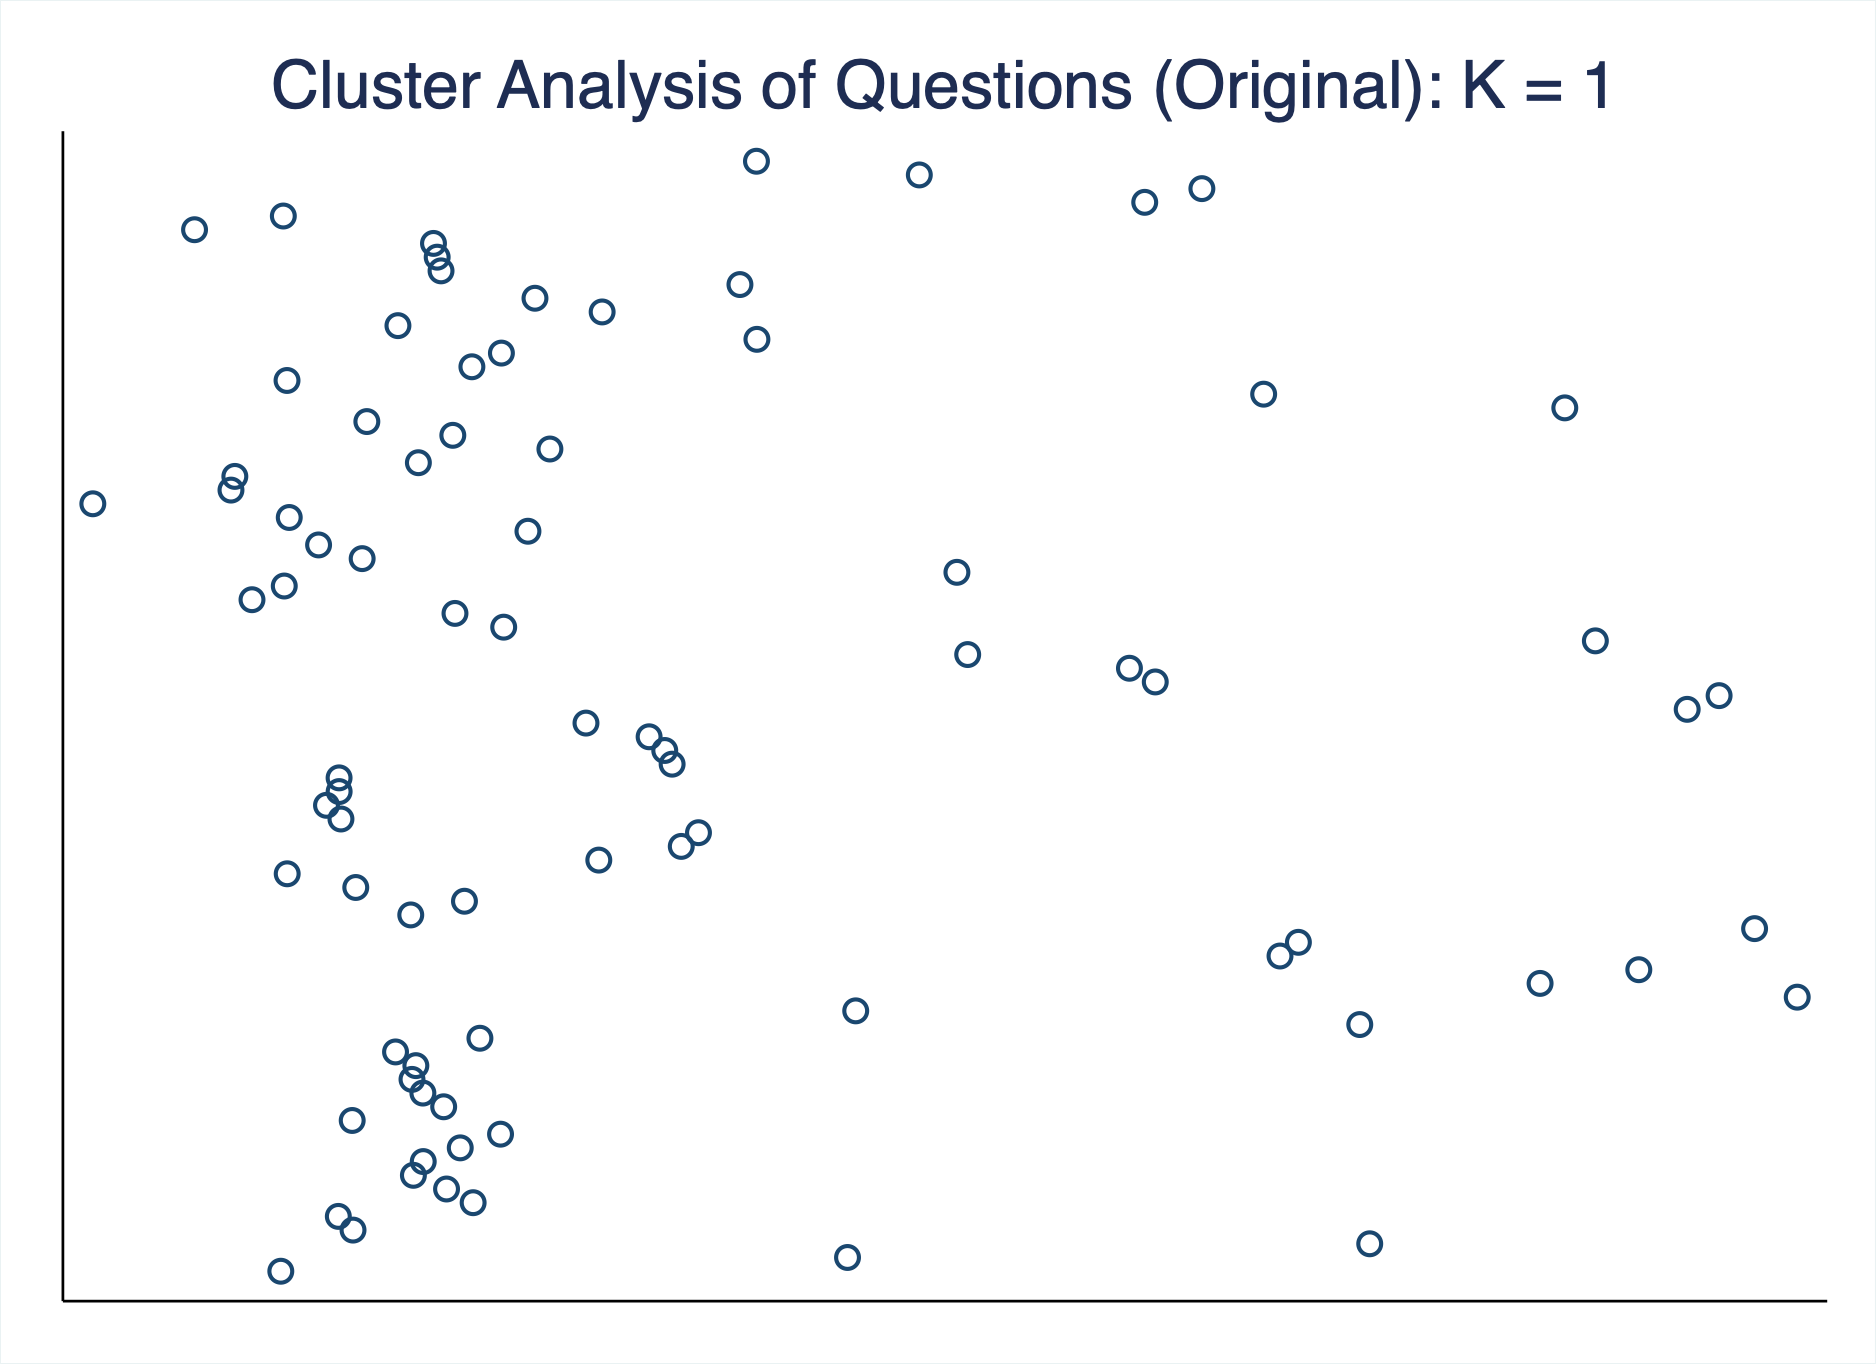
\includegraphics[scale=0.15]{CA_QuestionK1_ORI.png}
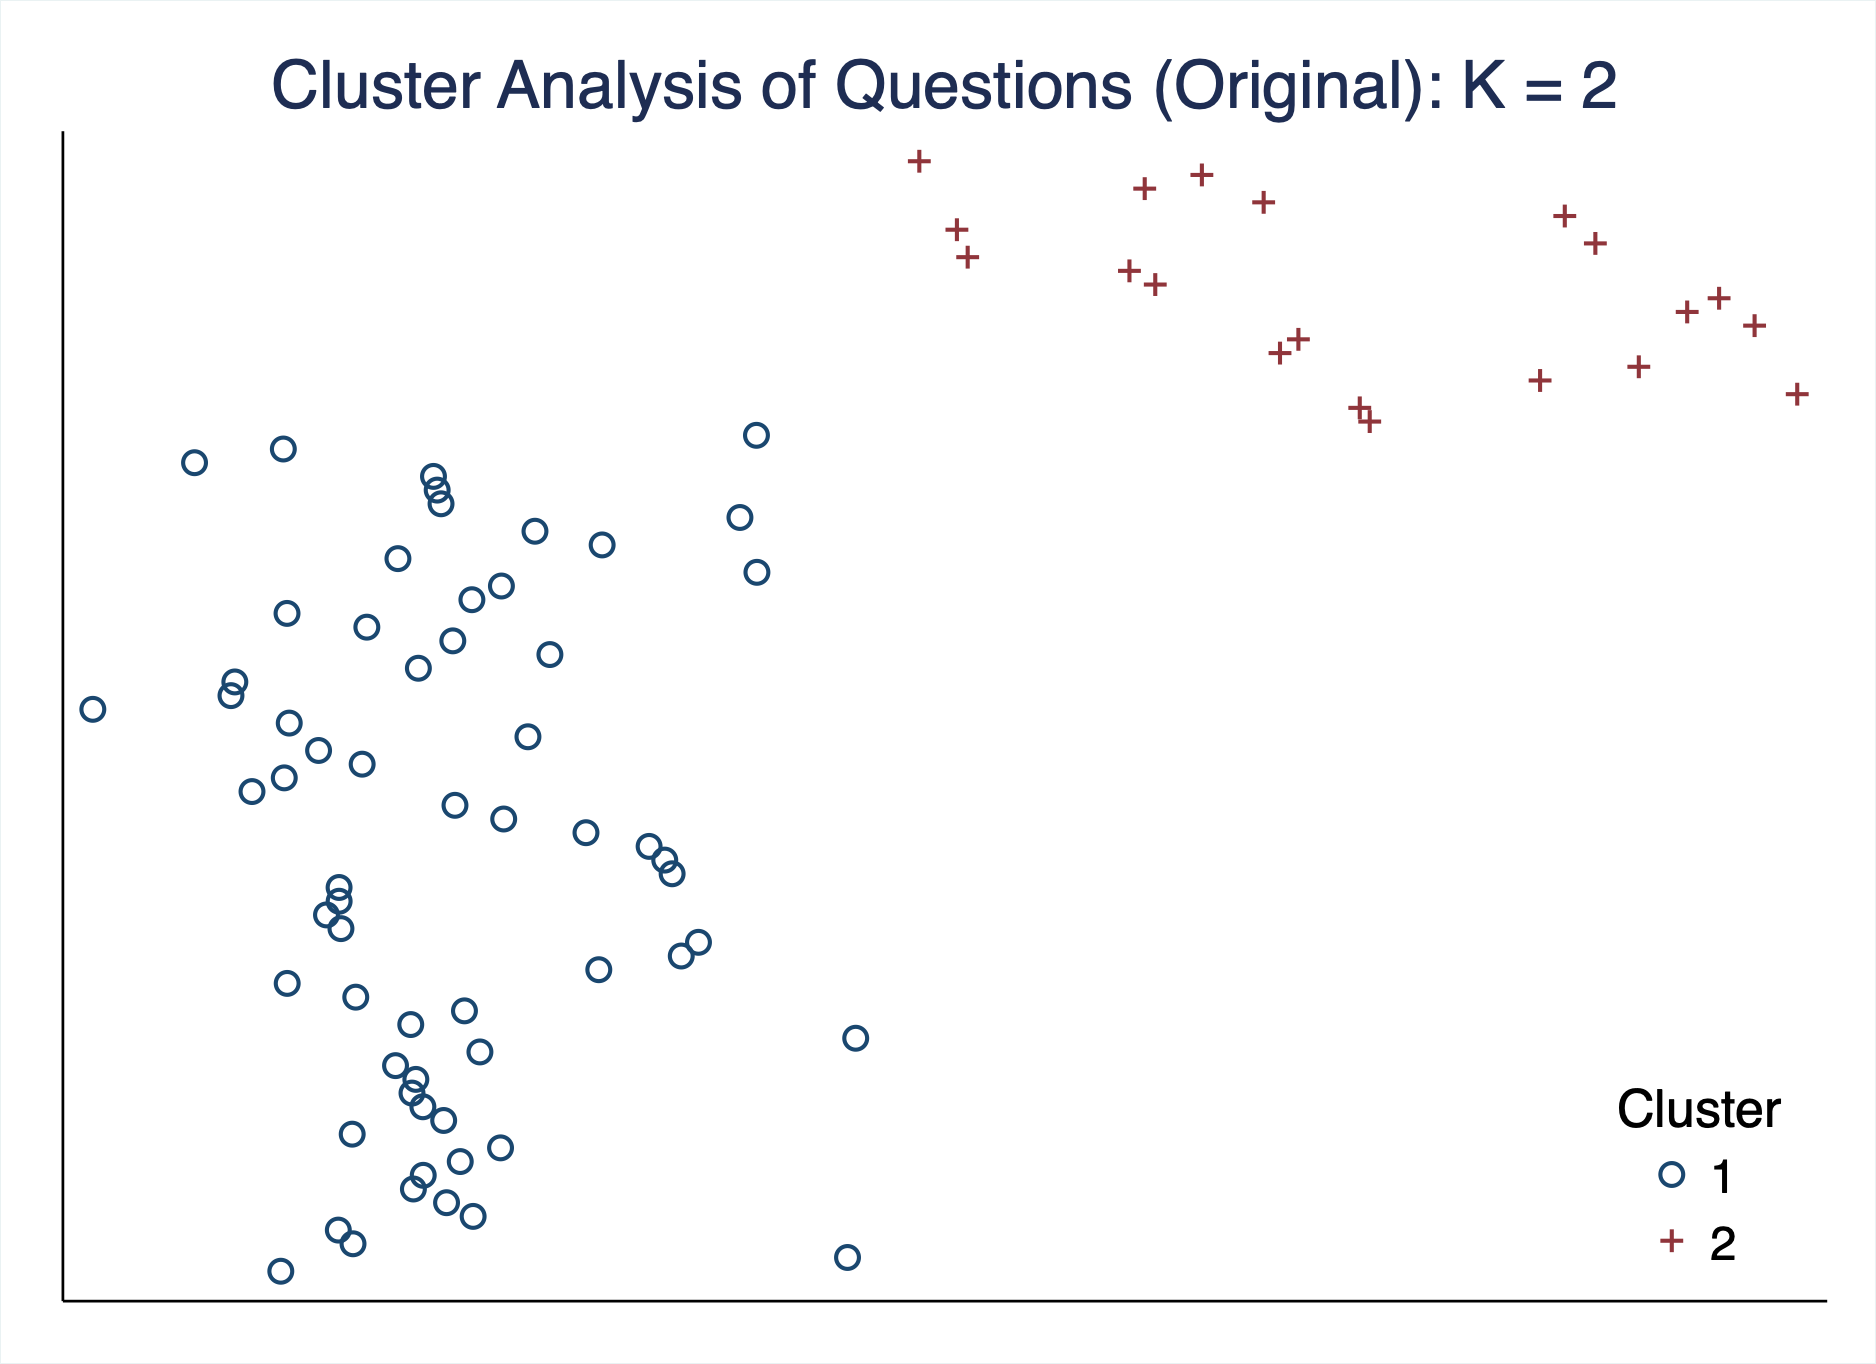
\includegraphics[scale=0.15]{CA_QuestionK2_ORI.png}
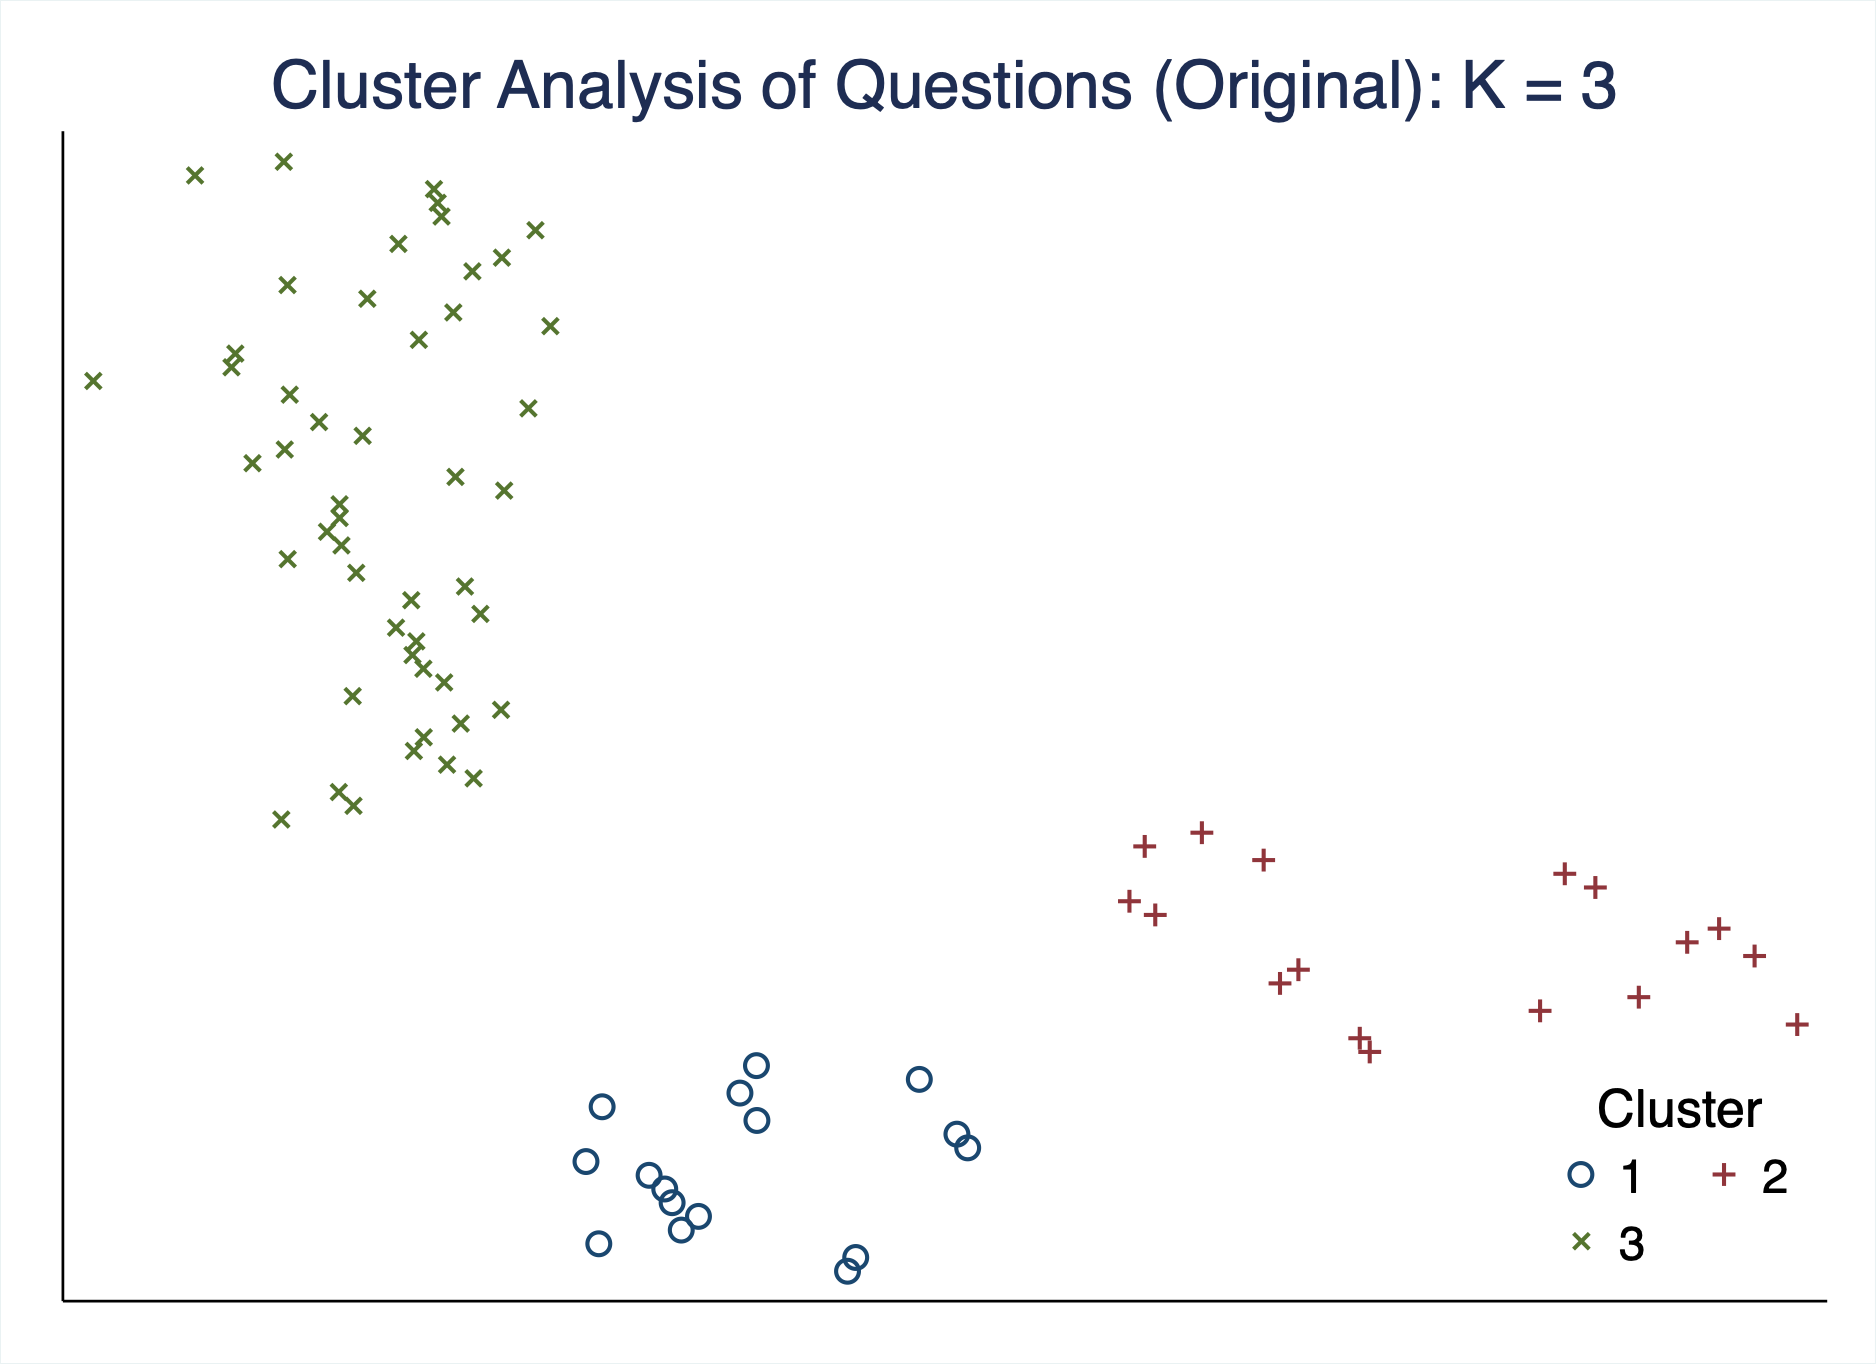
\includegraphics[scale=0.15]{CA_QuestionK3_ORI.png}
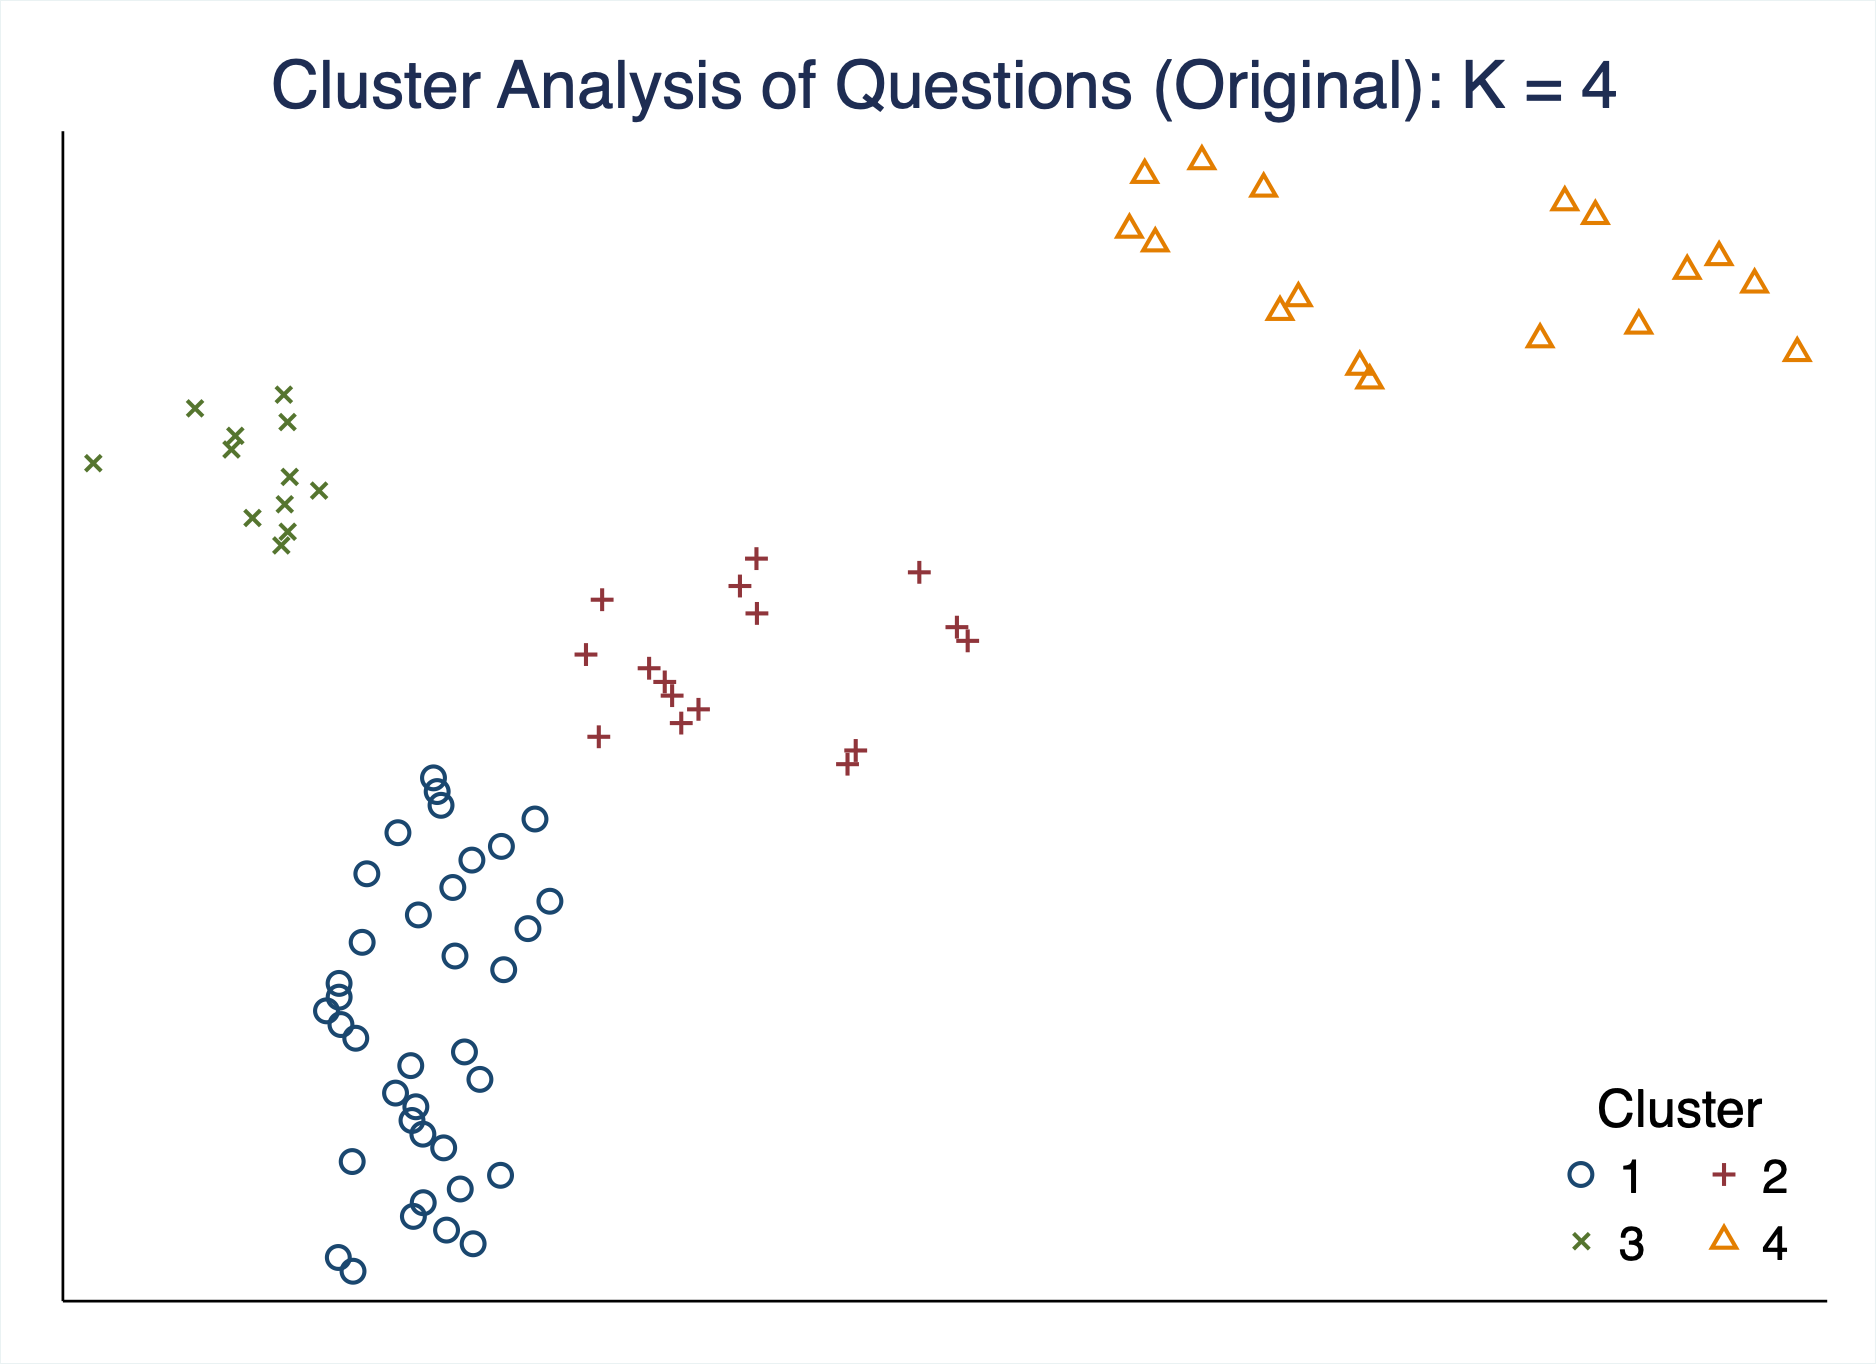
\includegraphics[scale=0.15]{CA_QuestionK4_ORI.png}
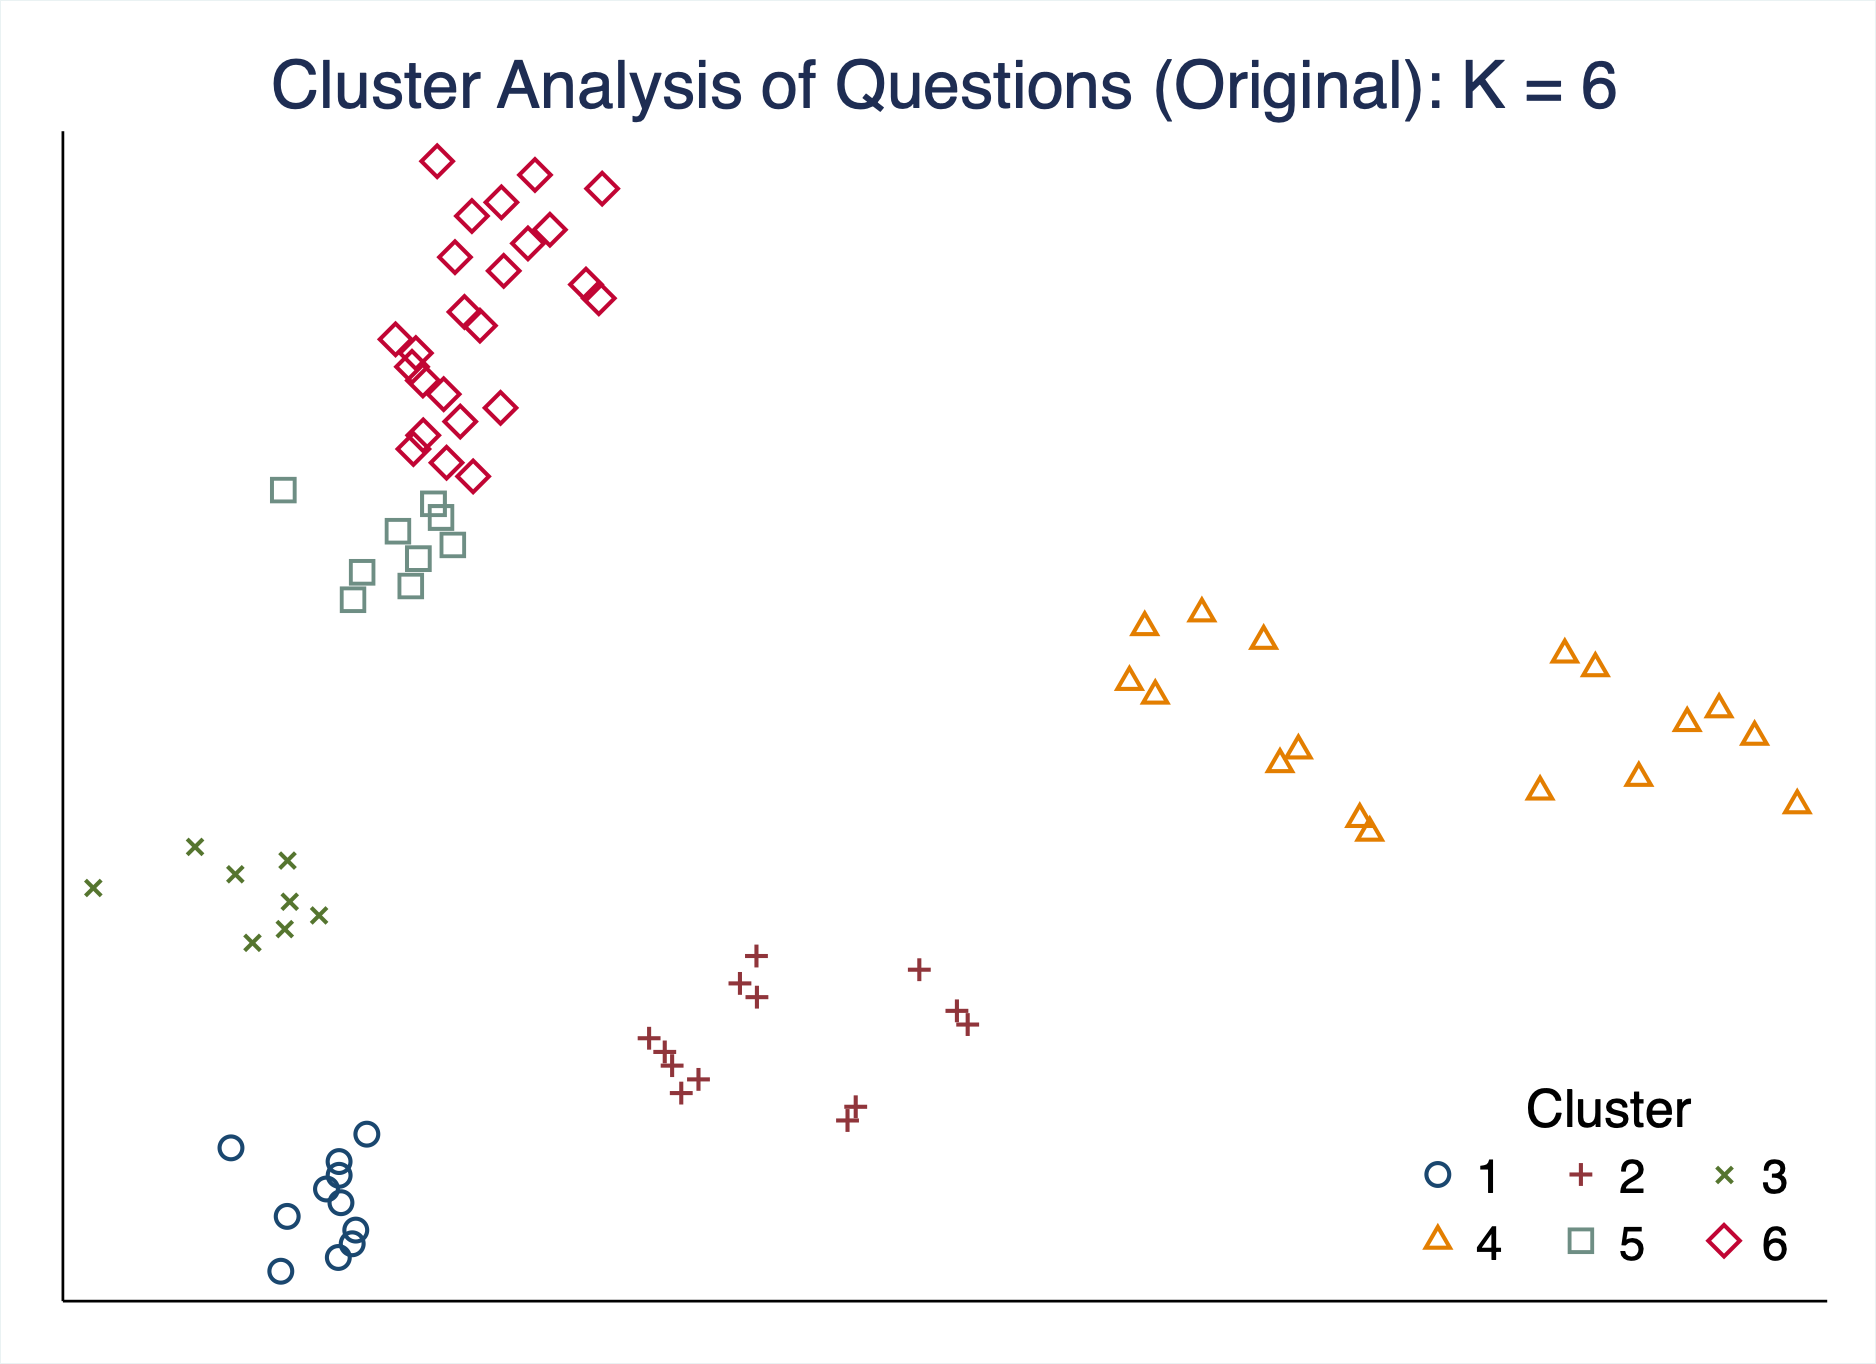
\includegraphics[scale=0.15]{CA_QuestionK6_ORI.png}
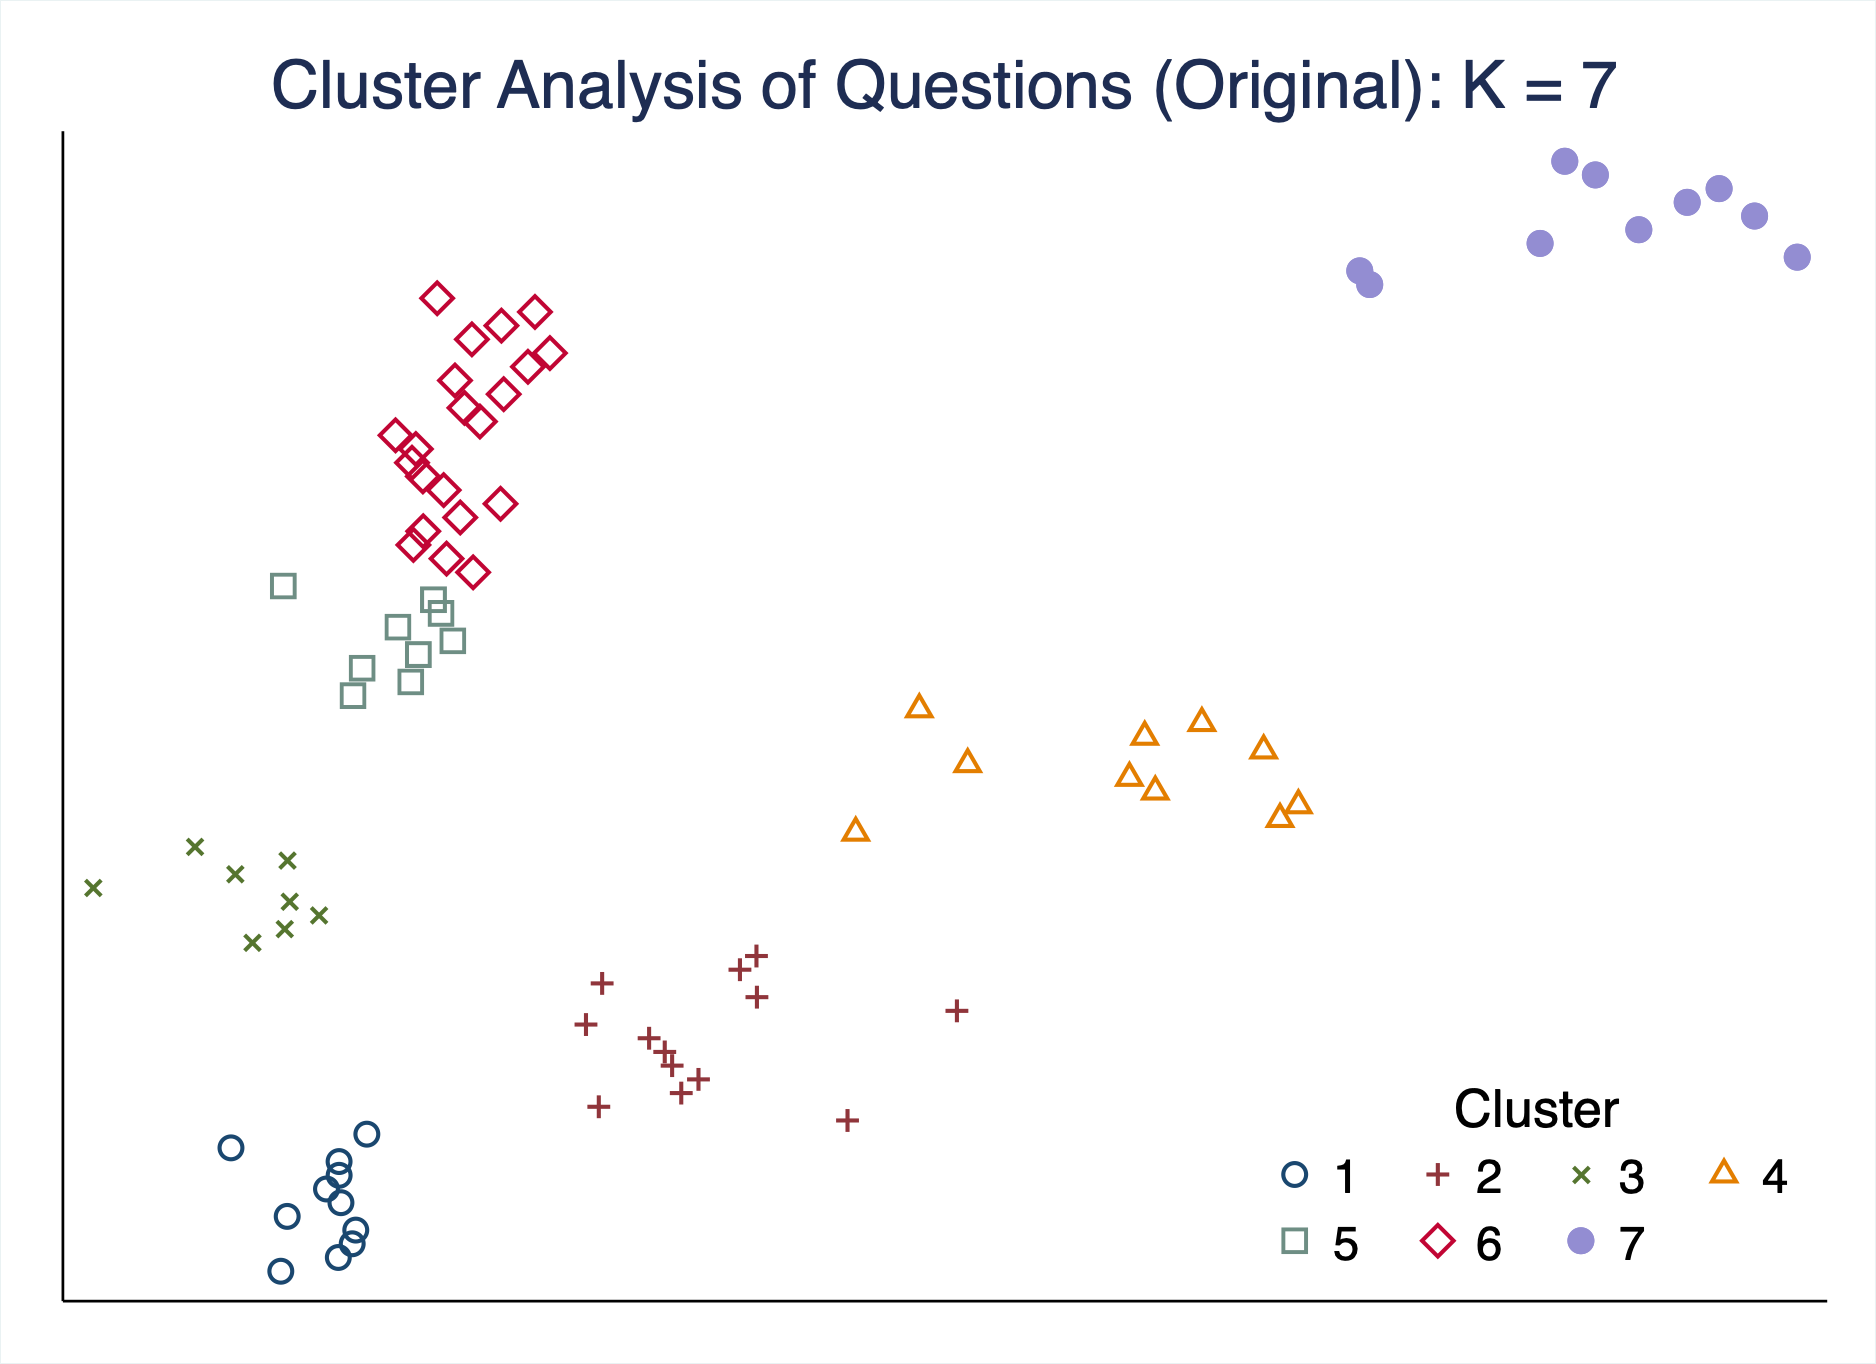
\includegraphics[scale=0.15]{CA_QuestionK7_ORI.png}
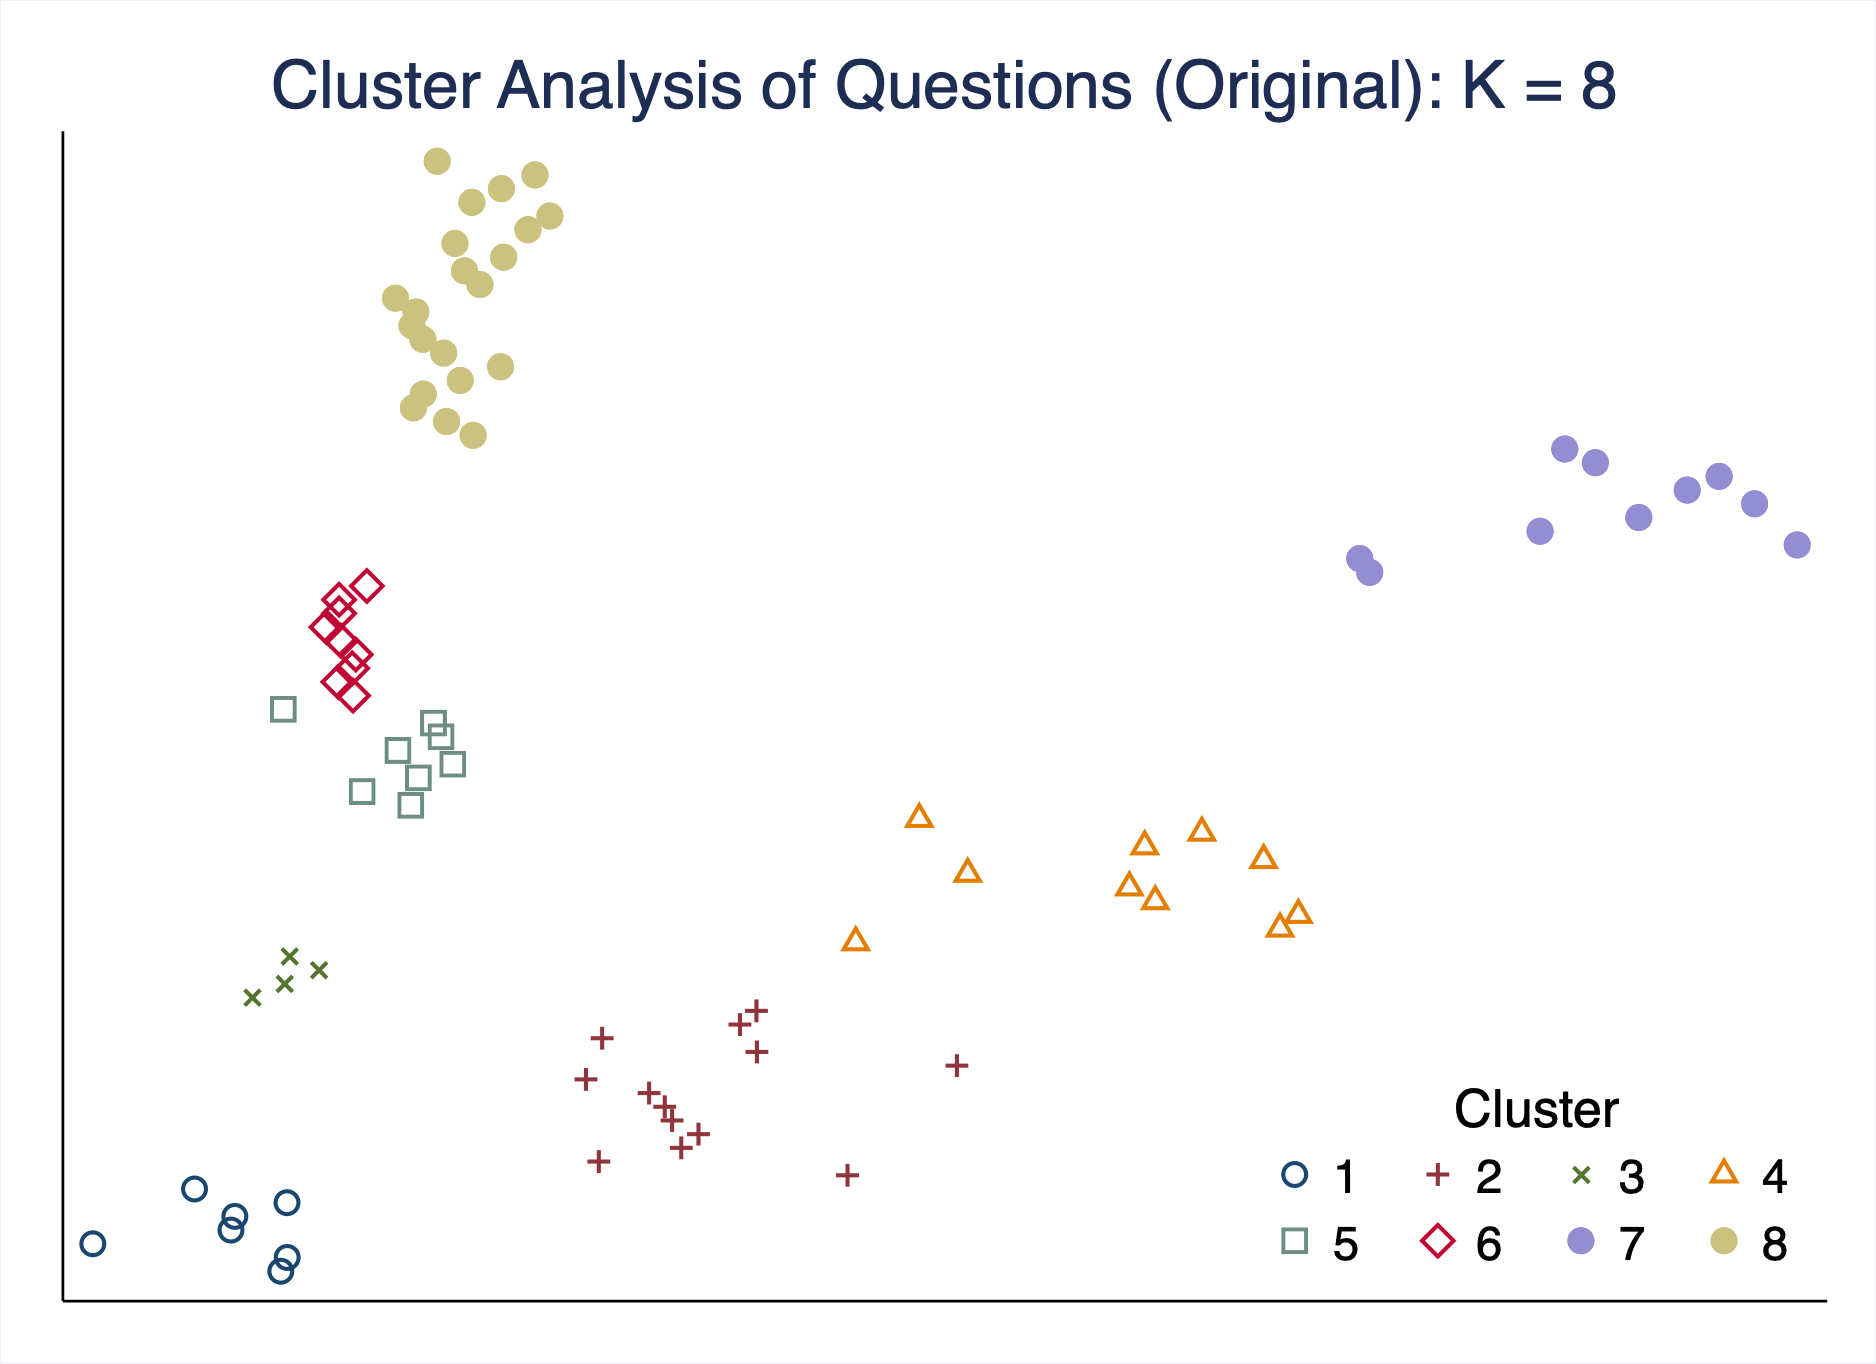
\includegraphics[scale=0.15]{CA_QuestionK8_ORI.png}
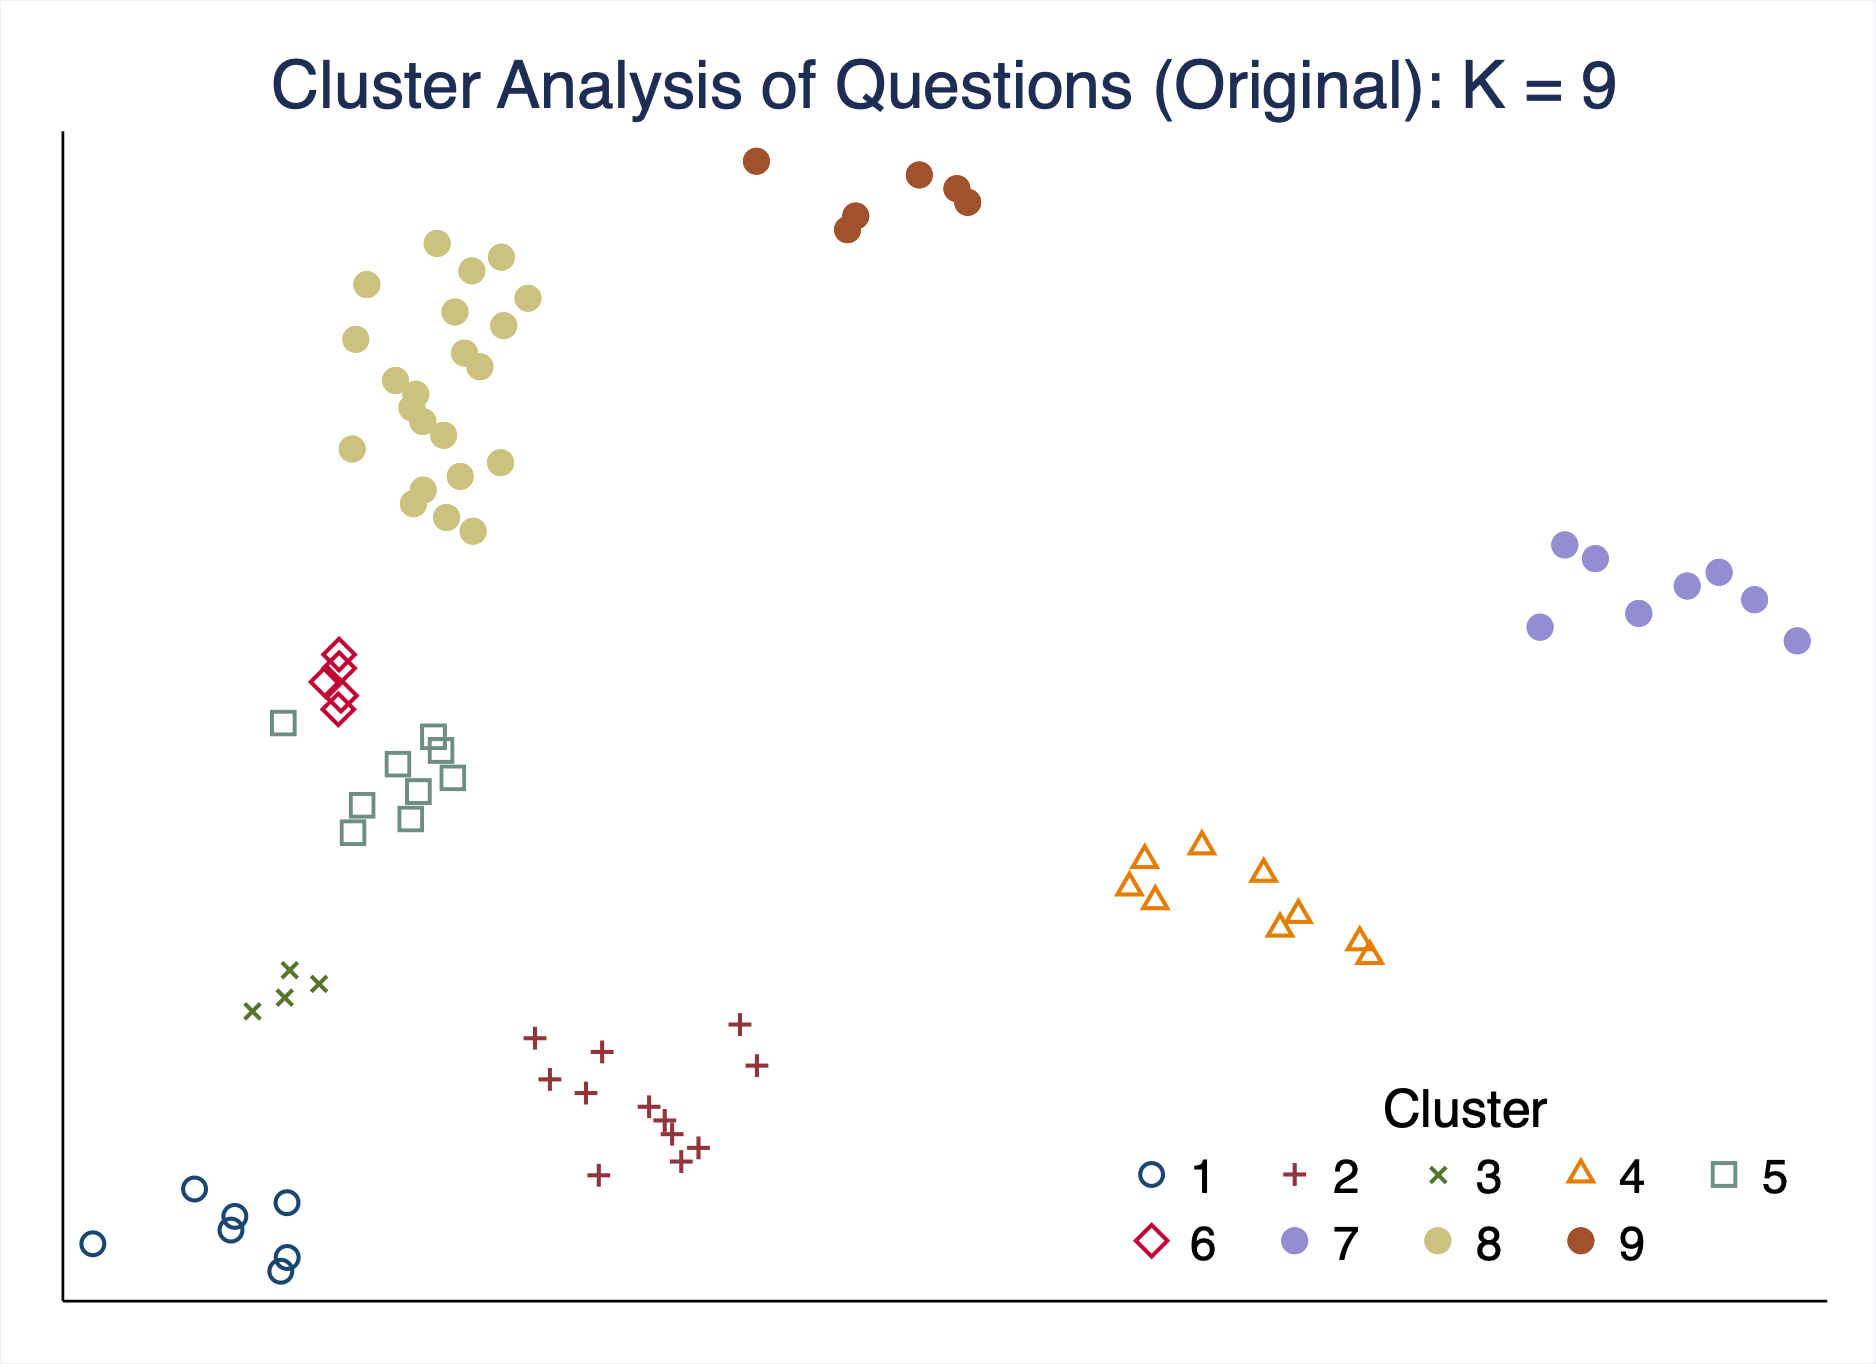
\includegraphics[scale=0.15]{CA_QuestionK9_ORI.png}
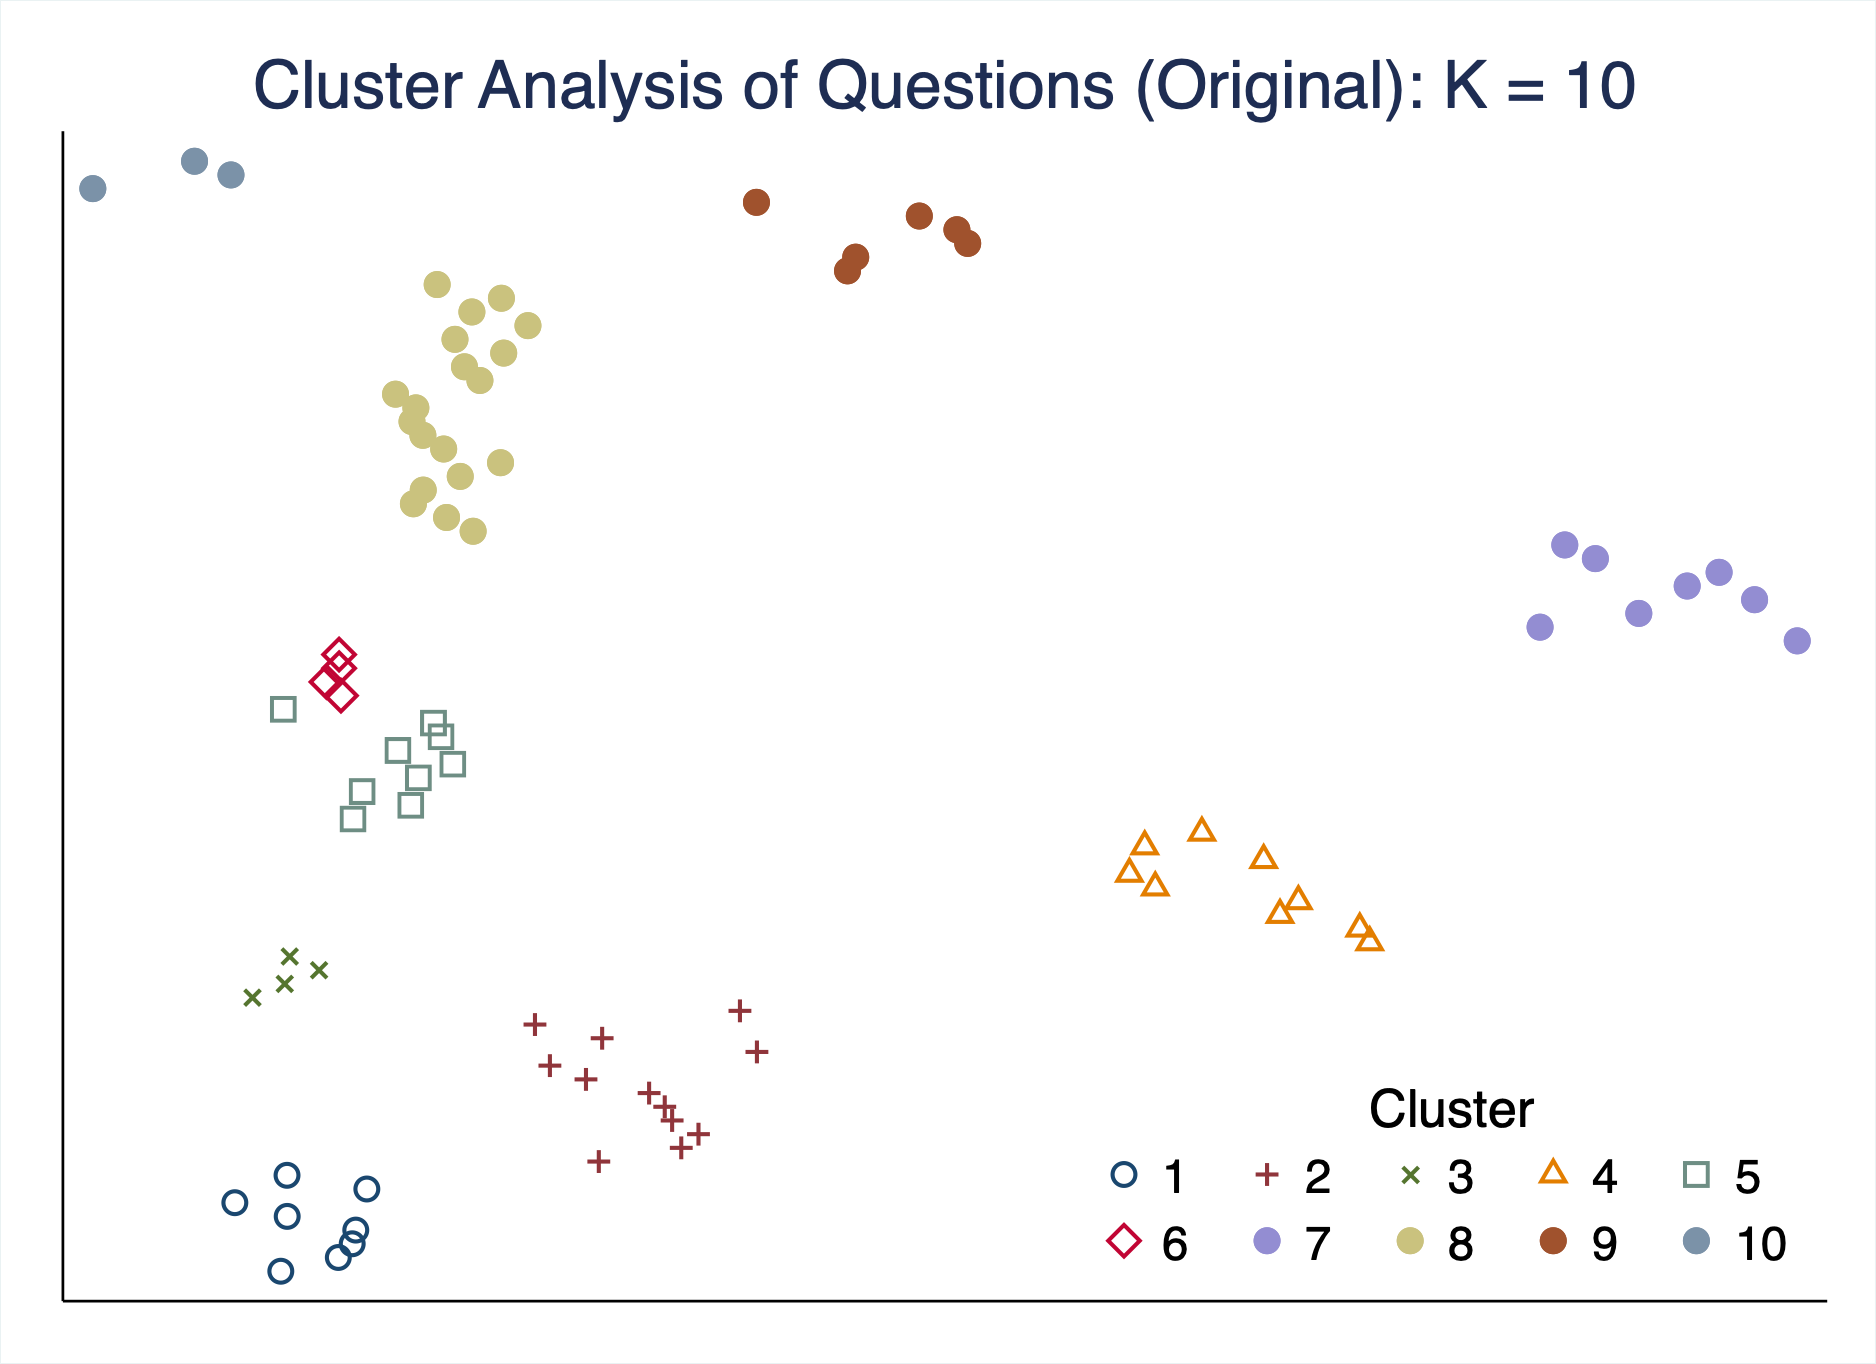
\includegraphics[scale=0.15]{CA_QuestionK10_ORI.png}
\end{center}
\end{figure}  

Figure 1 shows the cluster analysis when grouping the questions for different numbers of clusters. The x-axis is the means of each question, and the y-axis is a random number assignment based on groups. The top left figure is when the data has not been clustered. Starting from K=4, we see that the data is well-clustered. My preference for the number of clusters is five depicted in figure 2 below. \\
\\
With five clusters, the questions are grouped into five clusters, namely, politics, life security, life importance, democracy and freedom, and traditional values explained in table 1. And as we can see, the cluster analysis provided a decent job in clustering questions that naturally belong to each other. However, there are some instances where this could be done better. For example, some of the questions regarding "confidence" are grouped into different categories, and some questions seem to not fit with the group theme. This problem could be made better with a unified scale of answers.

\begin{figure}  [h!]
\begin{center}
\caption{Cluster analysis of questions with non-normalized data (K=5)}
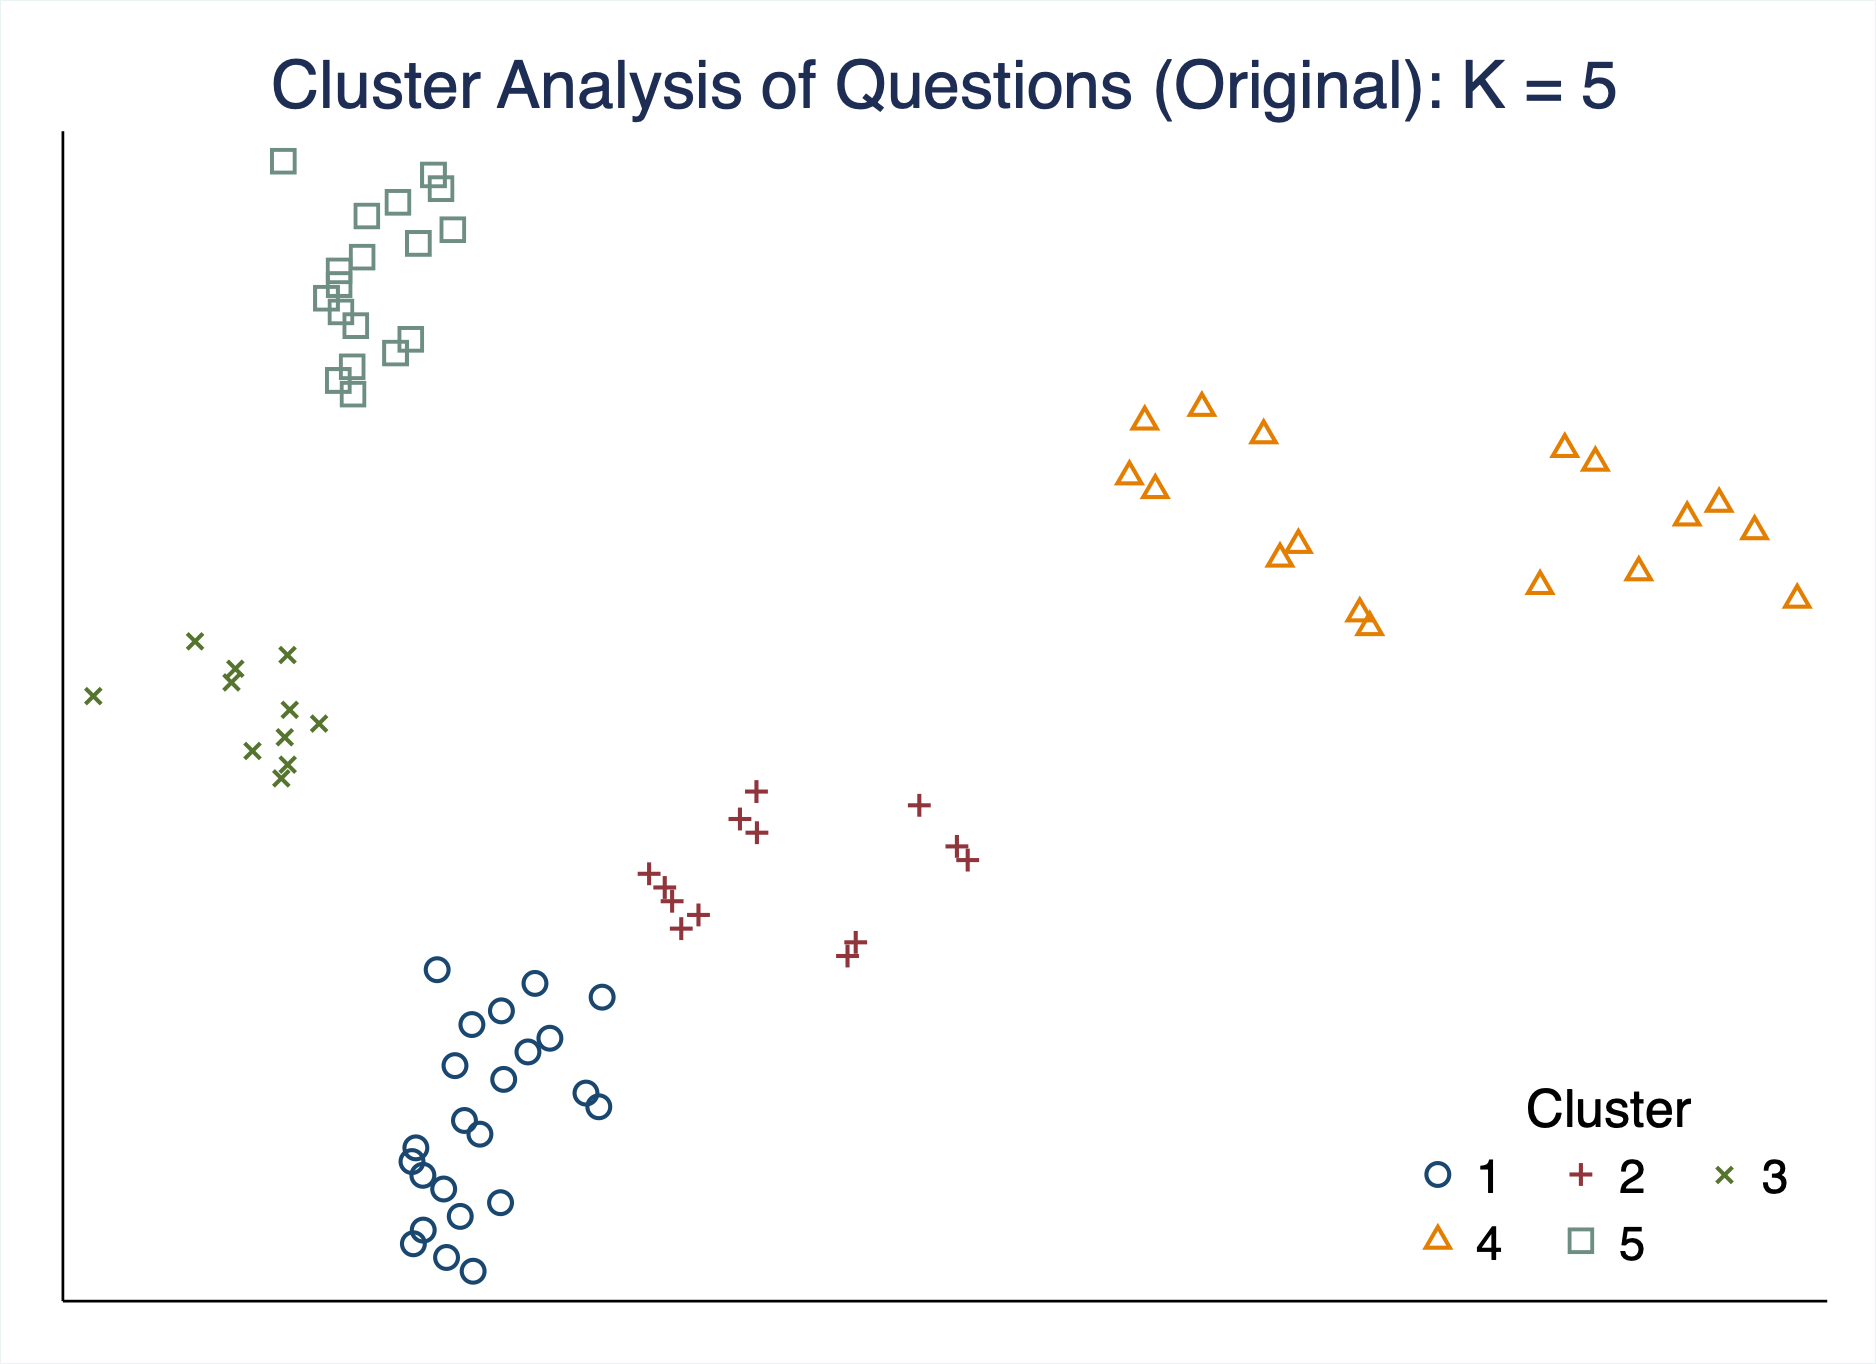
\includegraphics[scale=0.25]{CA_QuestionK5_ORI.png}
\end{center}
\end{figure}  

\begin{figure}  [h!]
\subsubsection{Country clustering}
\begin{center}
\caption{Cluster analysis of country with non-normalized data}
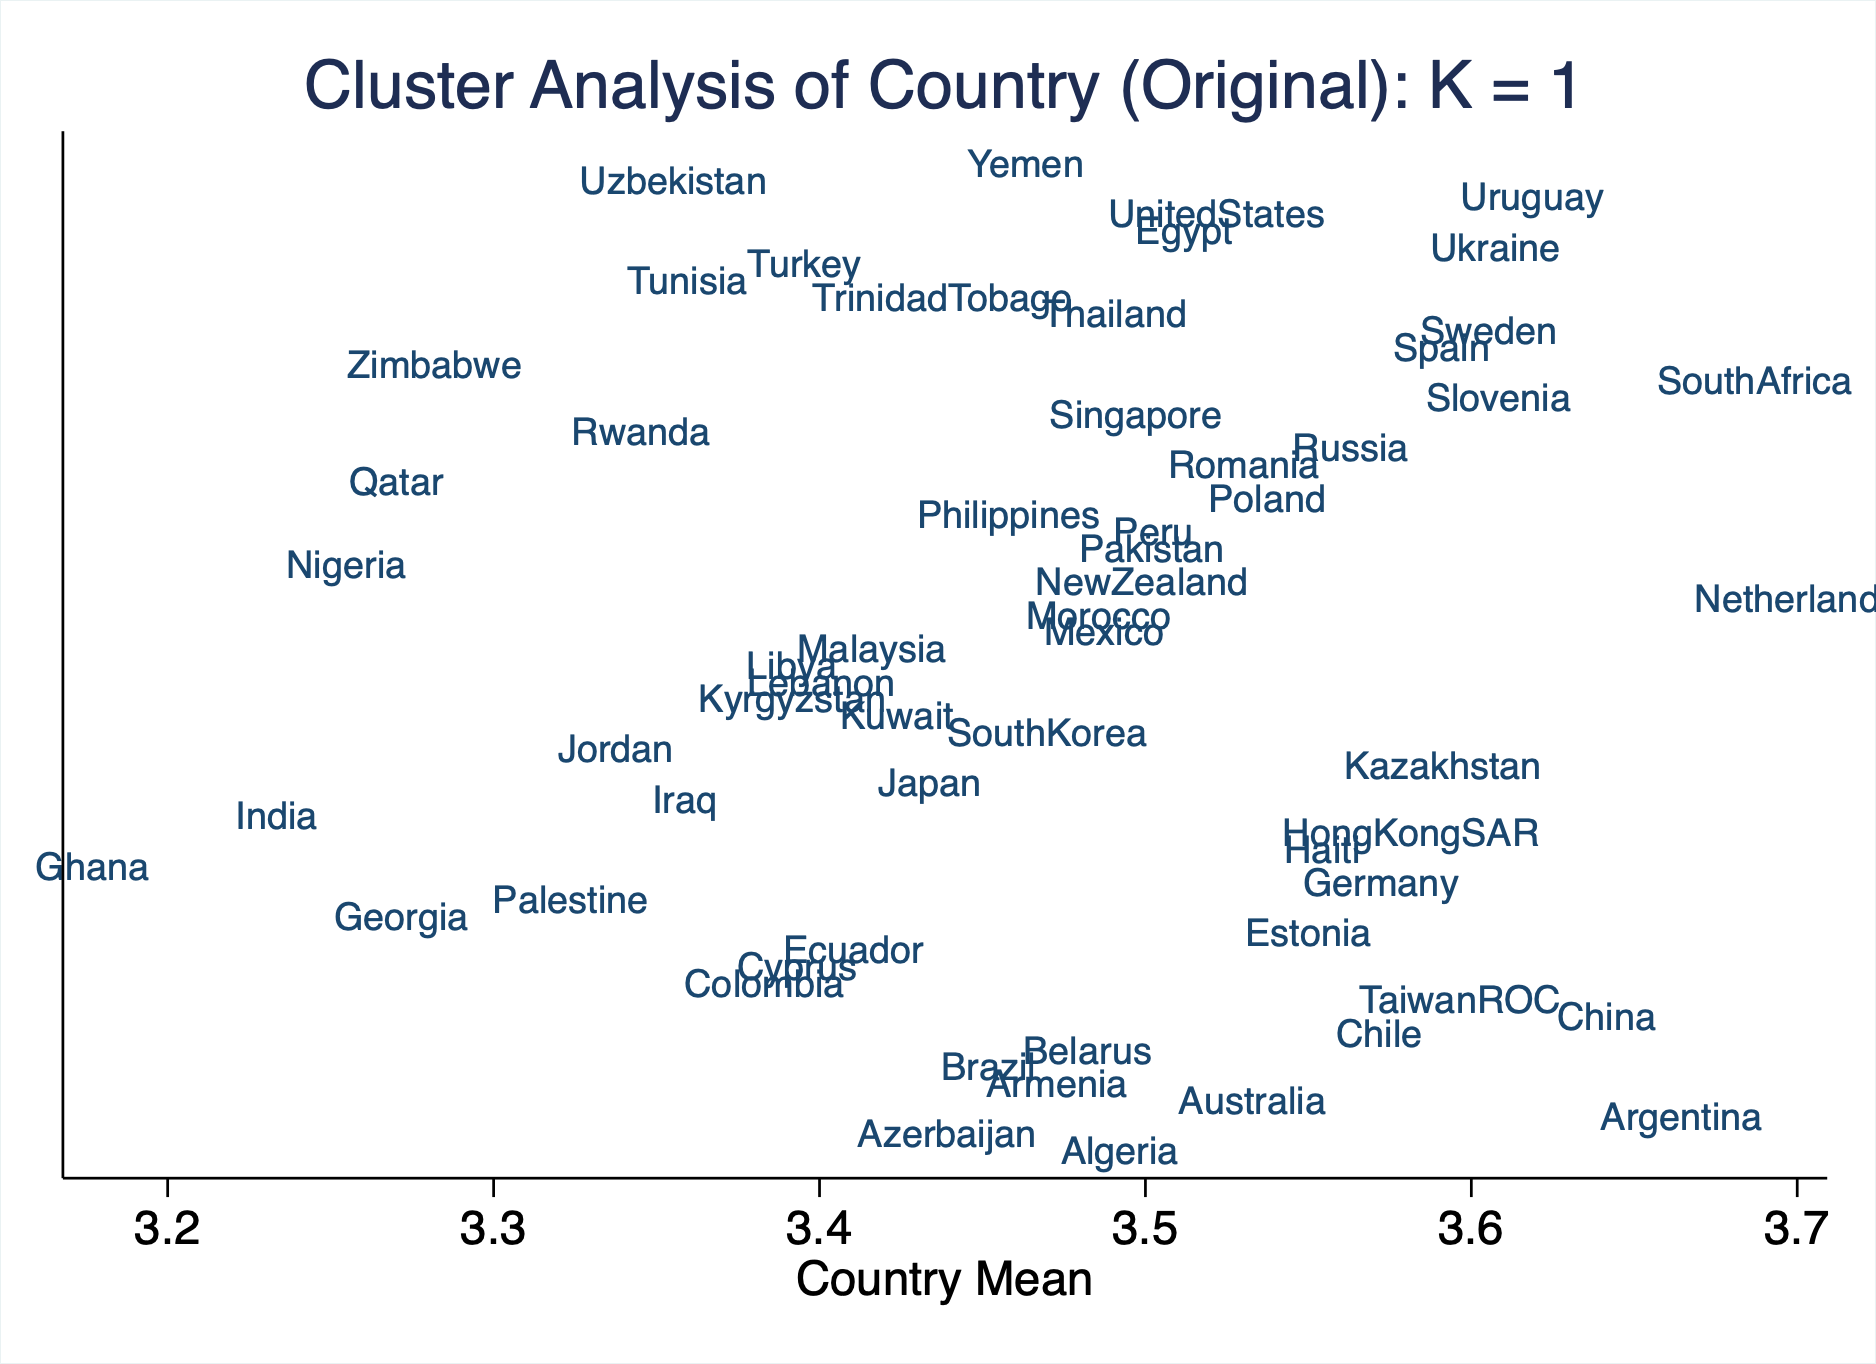
\includegraphics[scale=0.15]{CA_CountryK1_ORI.png}
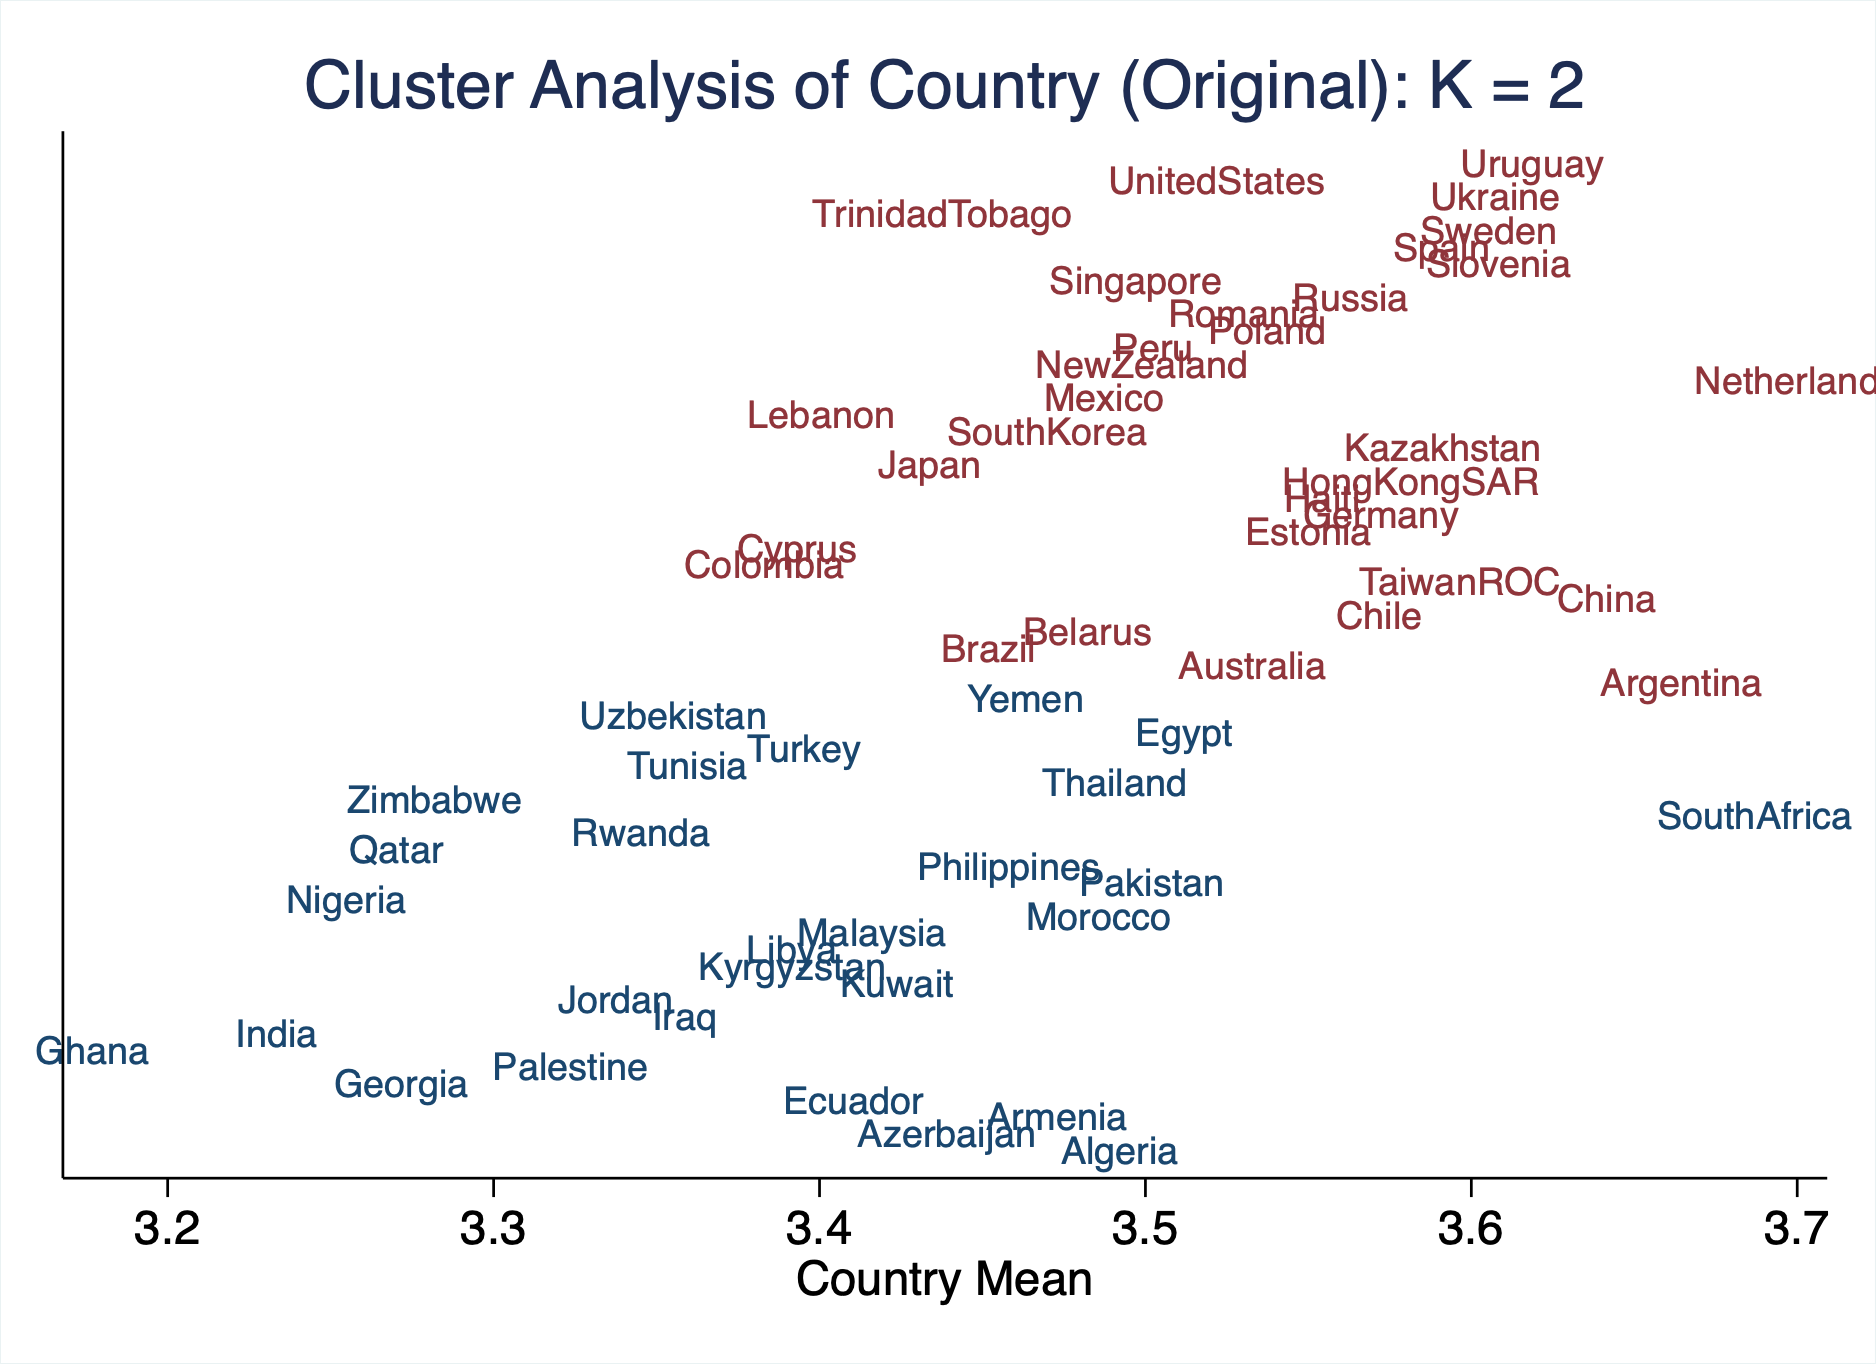
\includegraphics[scale=0.15]{CA_CountryK2_ORI.png}
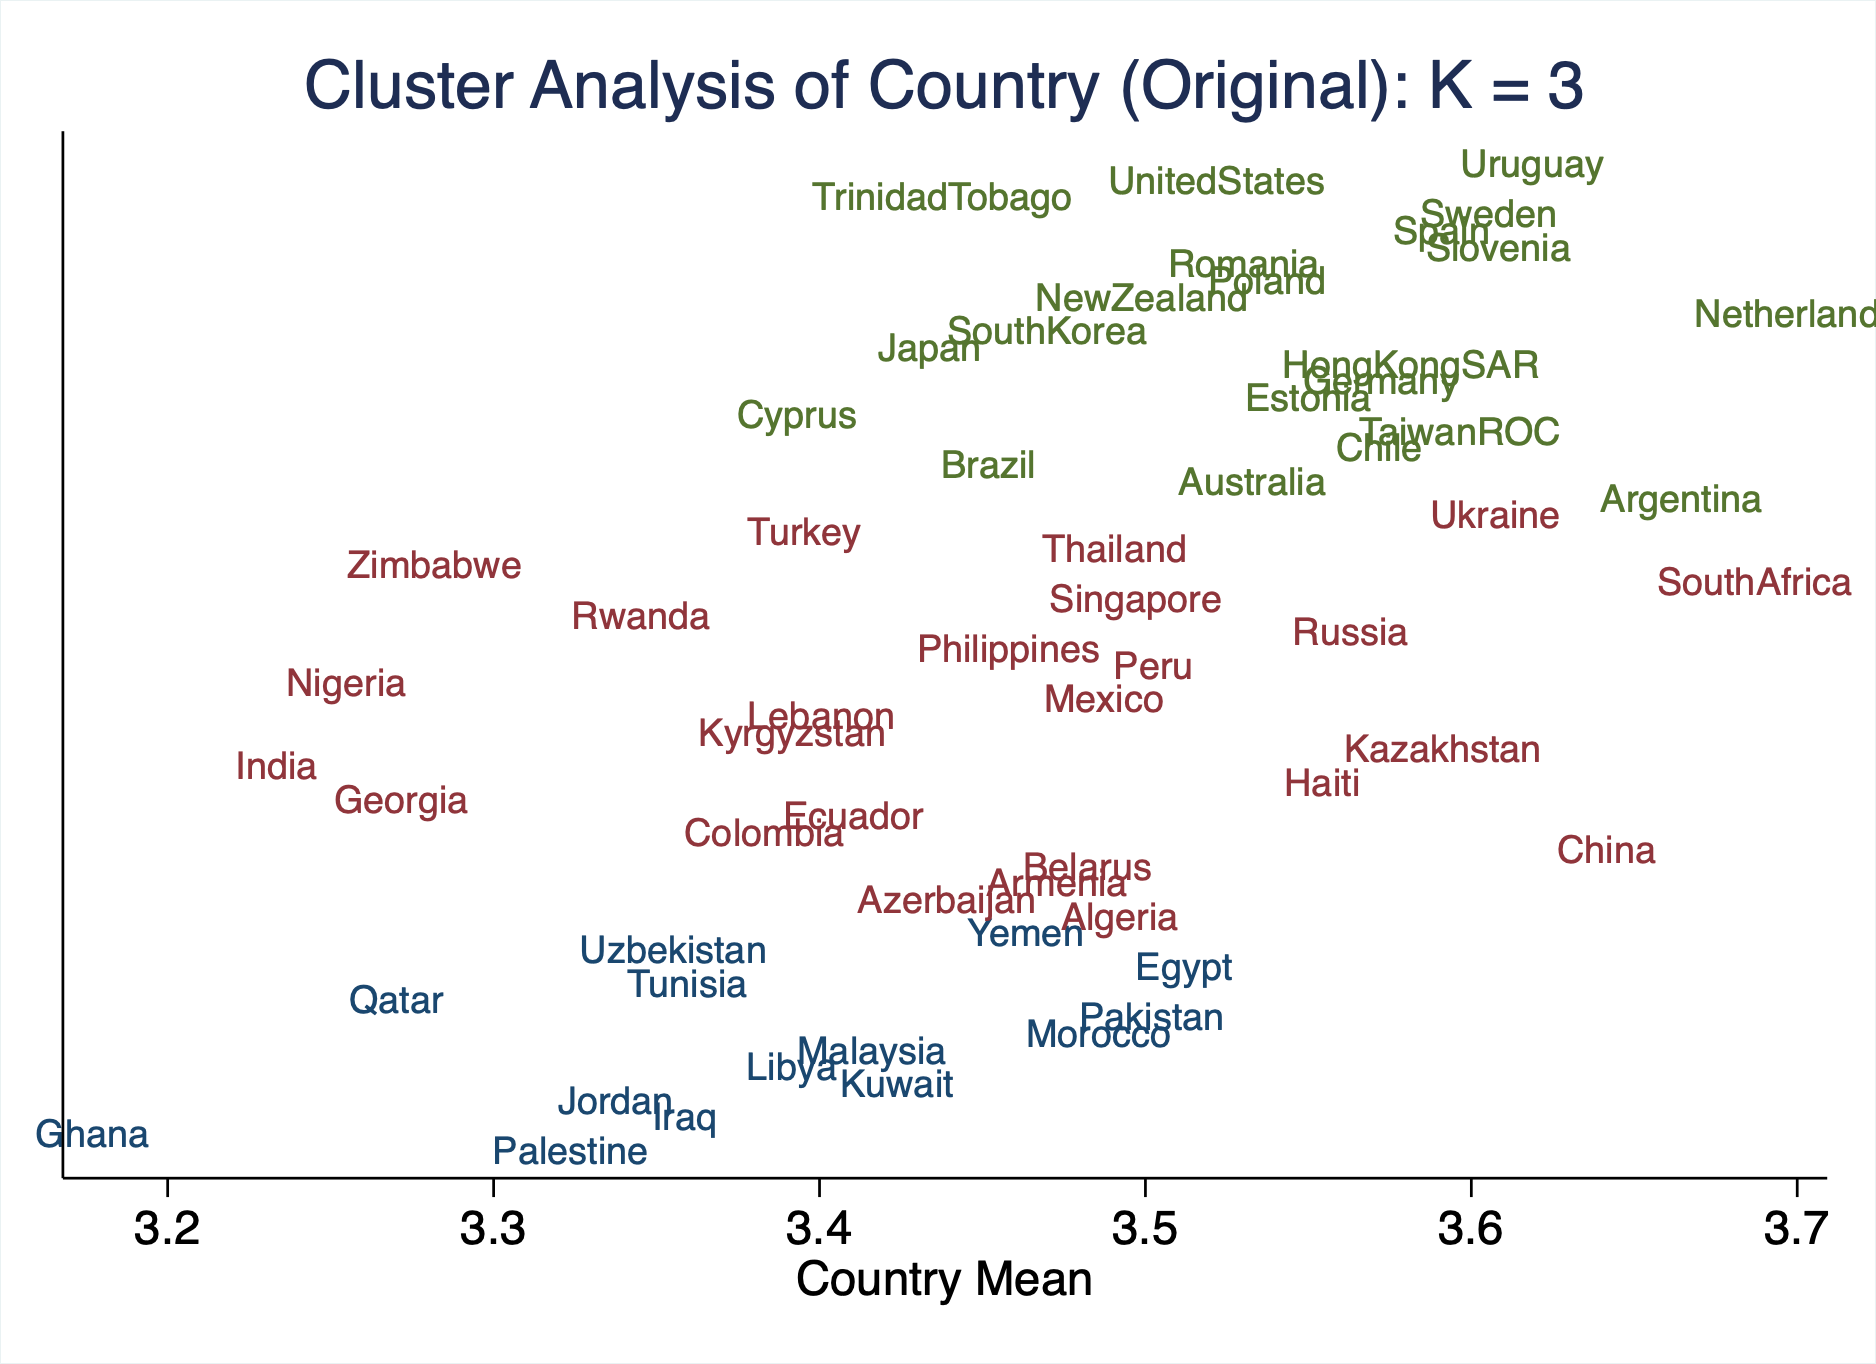
\includegraphics[scale=0.15]{CA_CountryK3_ORI.png}
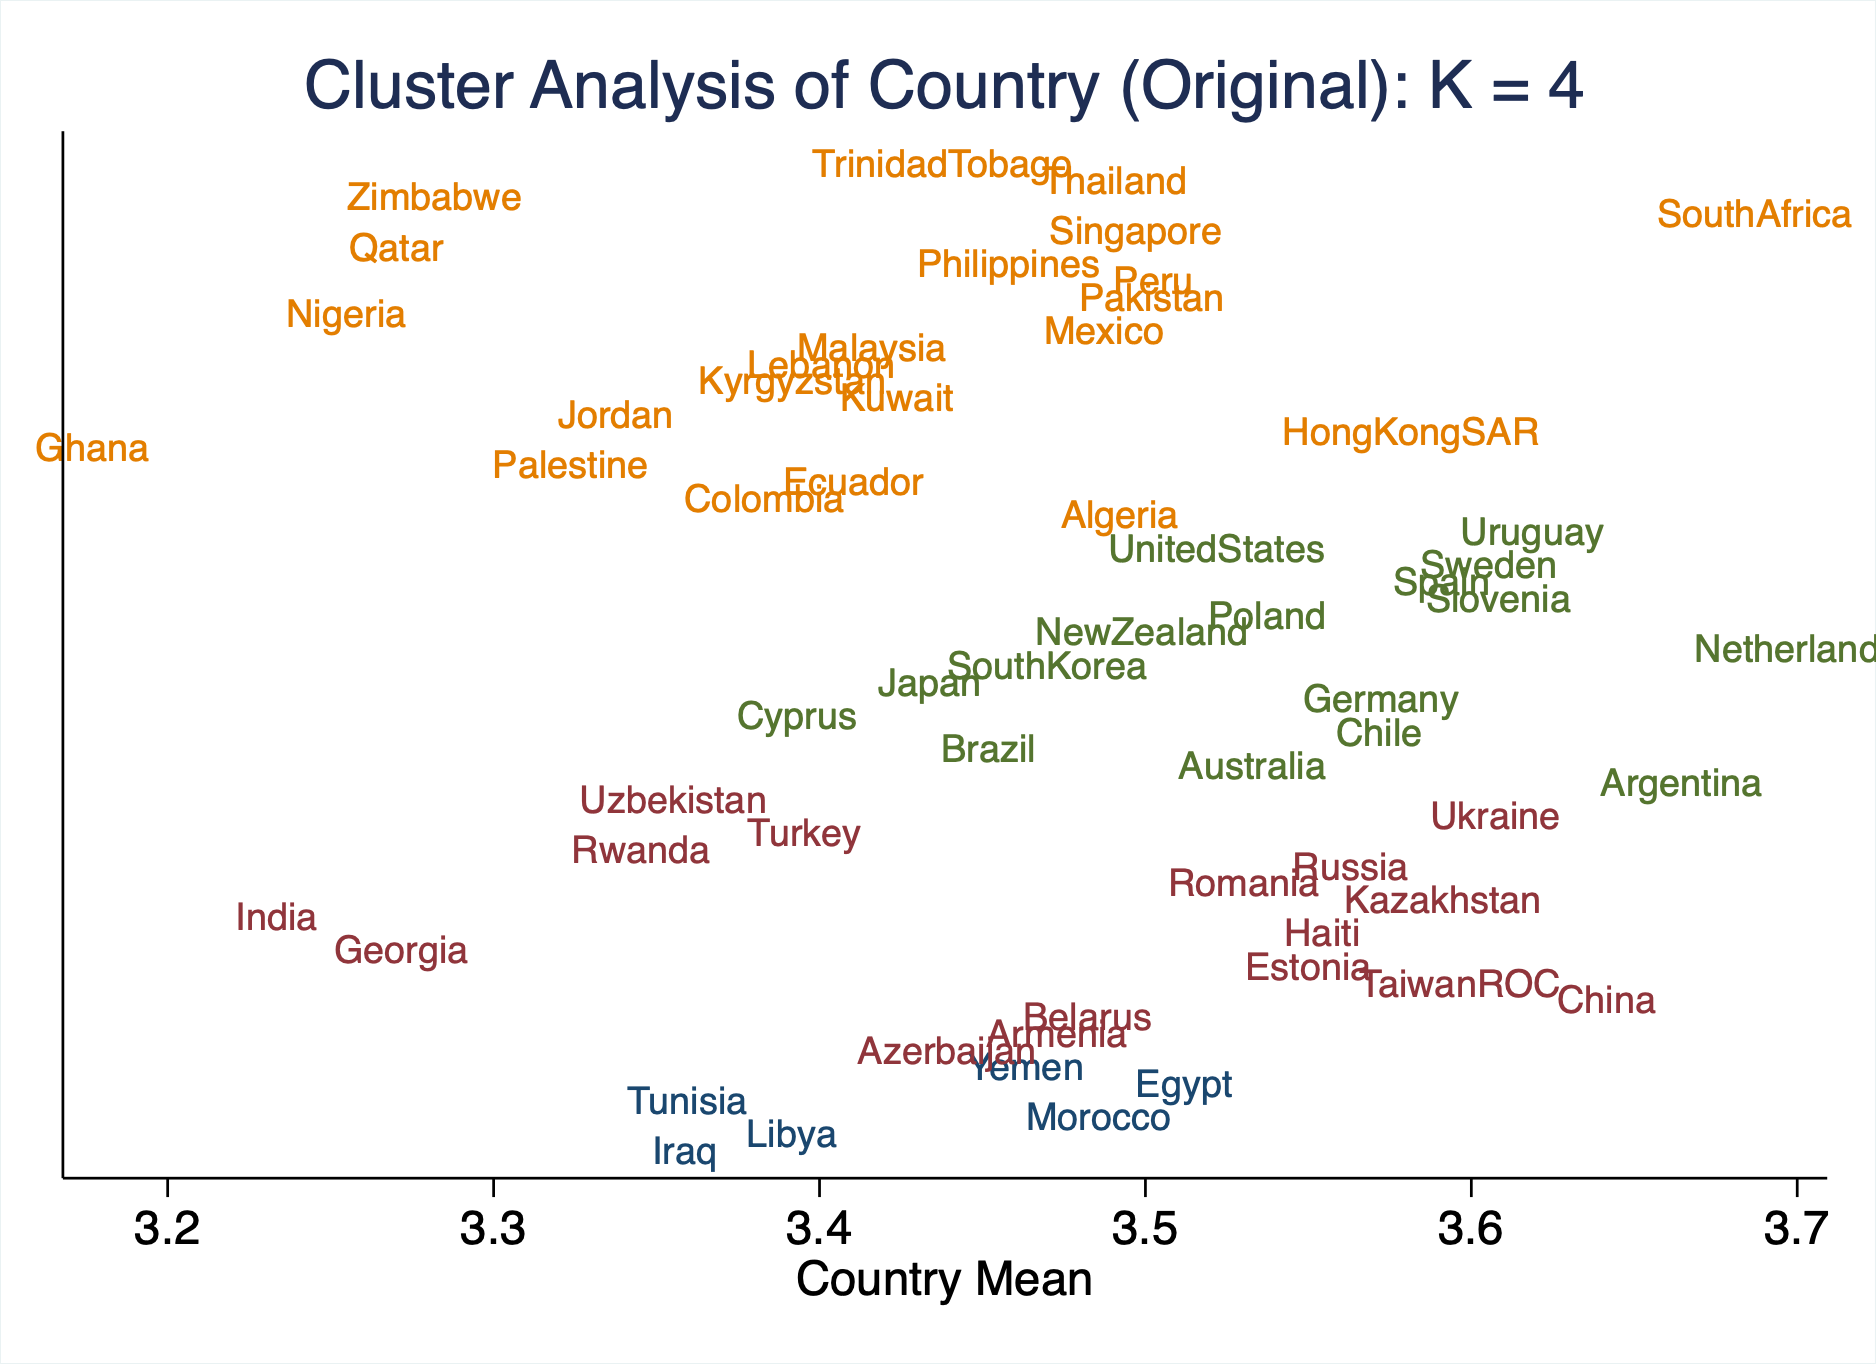
\includegraphics[scale=0.15]{CA_CountryK4_ORI.png}
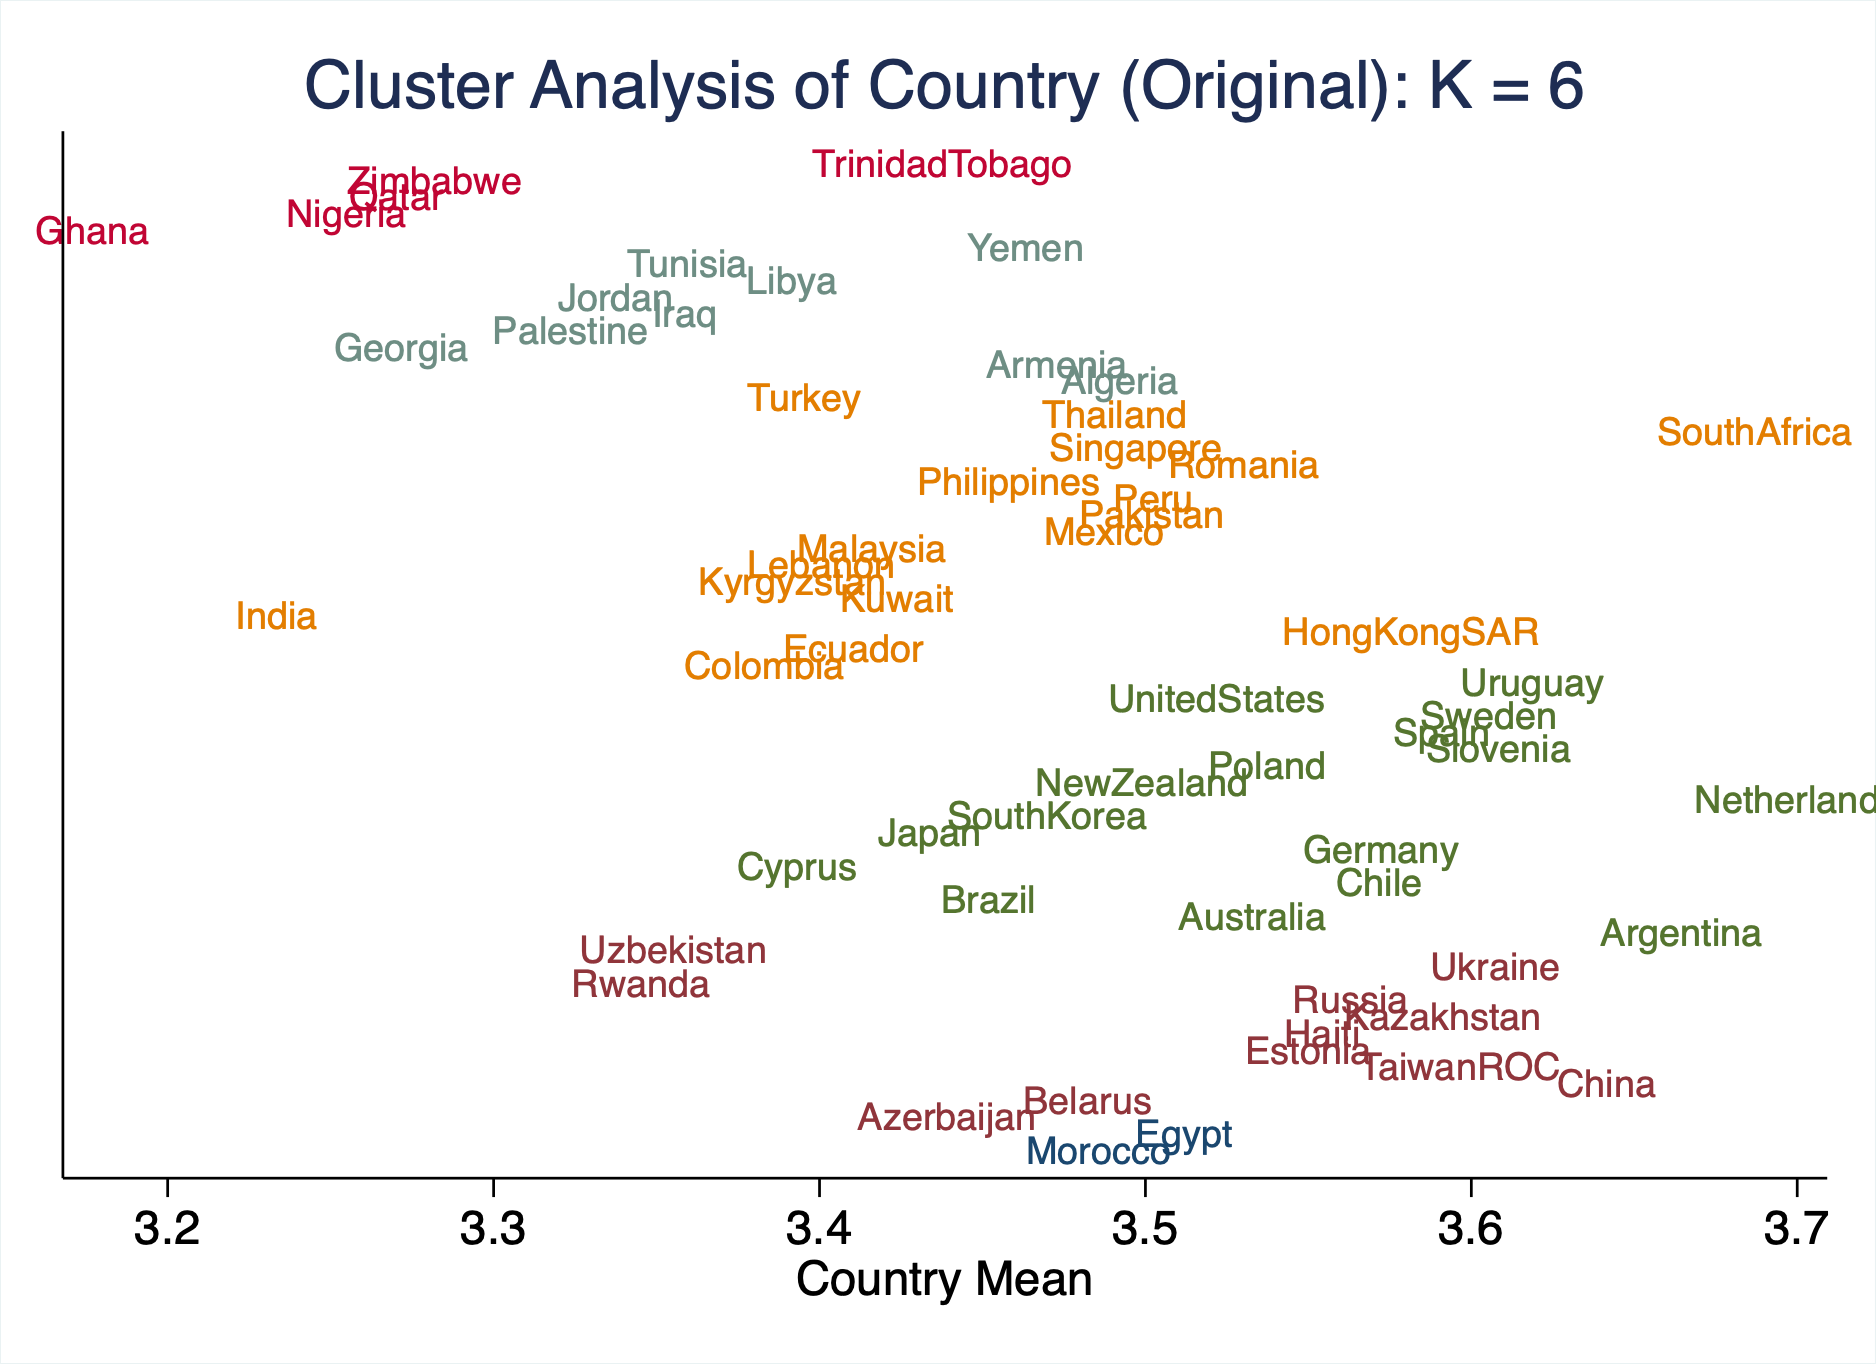
\includegraphics[scale=0.15]{CA_CountryK6_ORI.png}
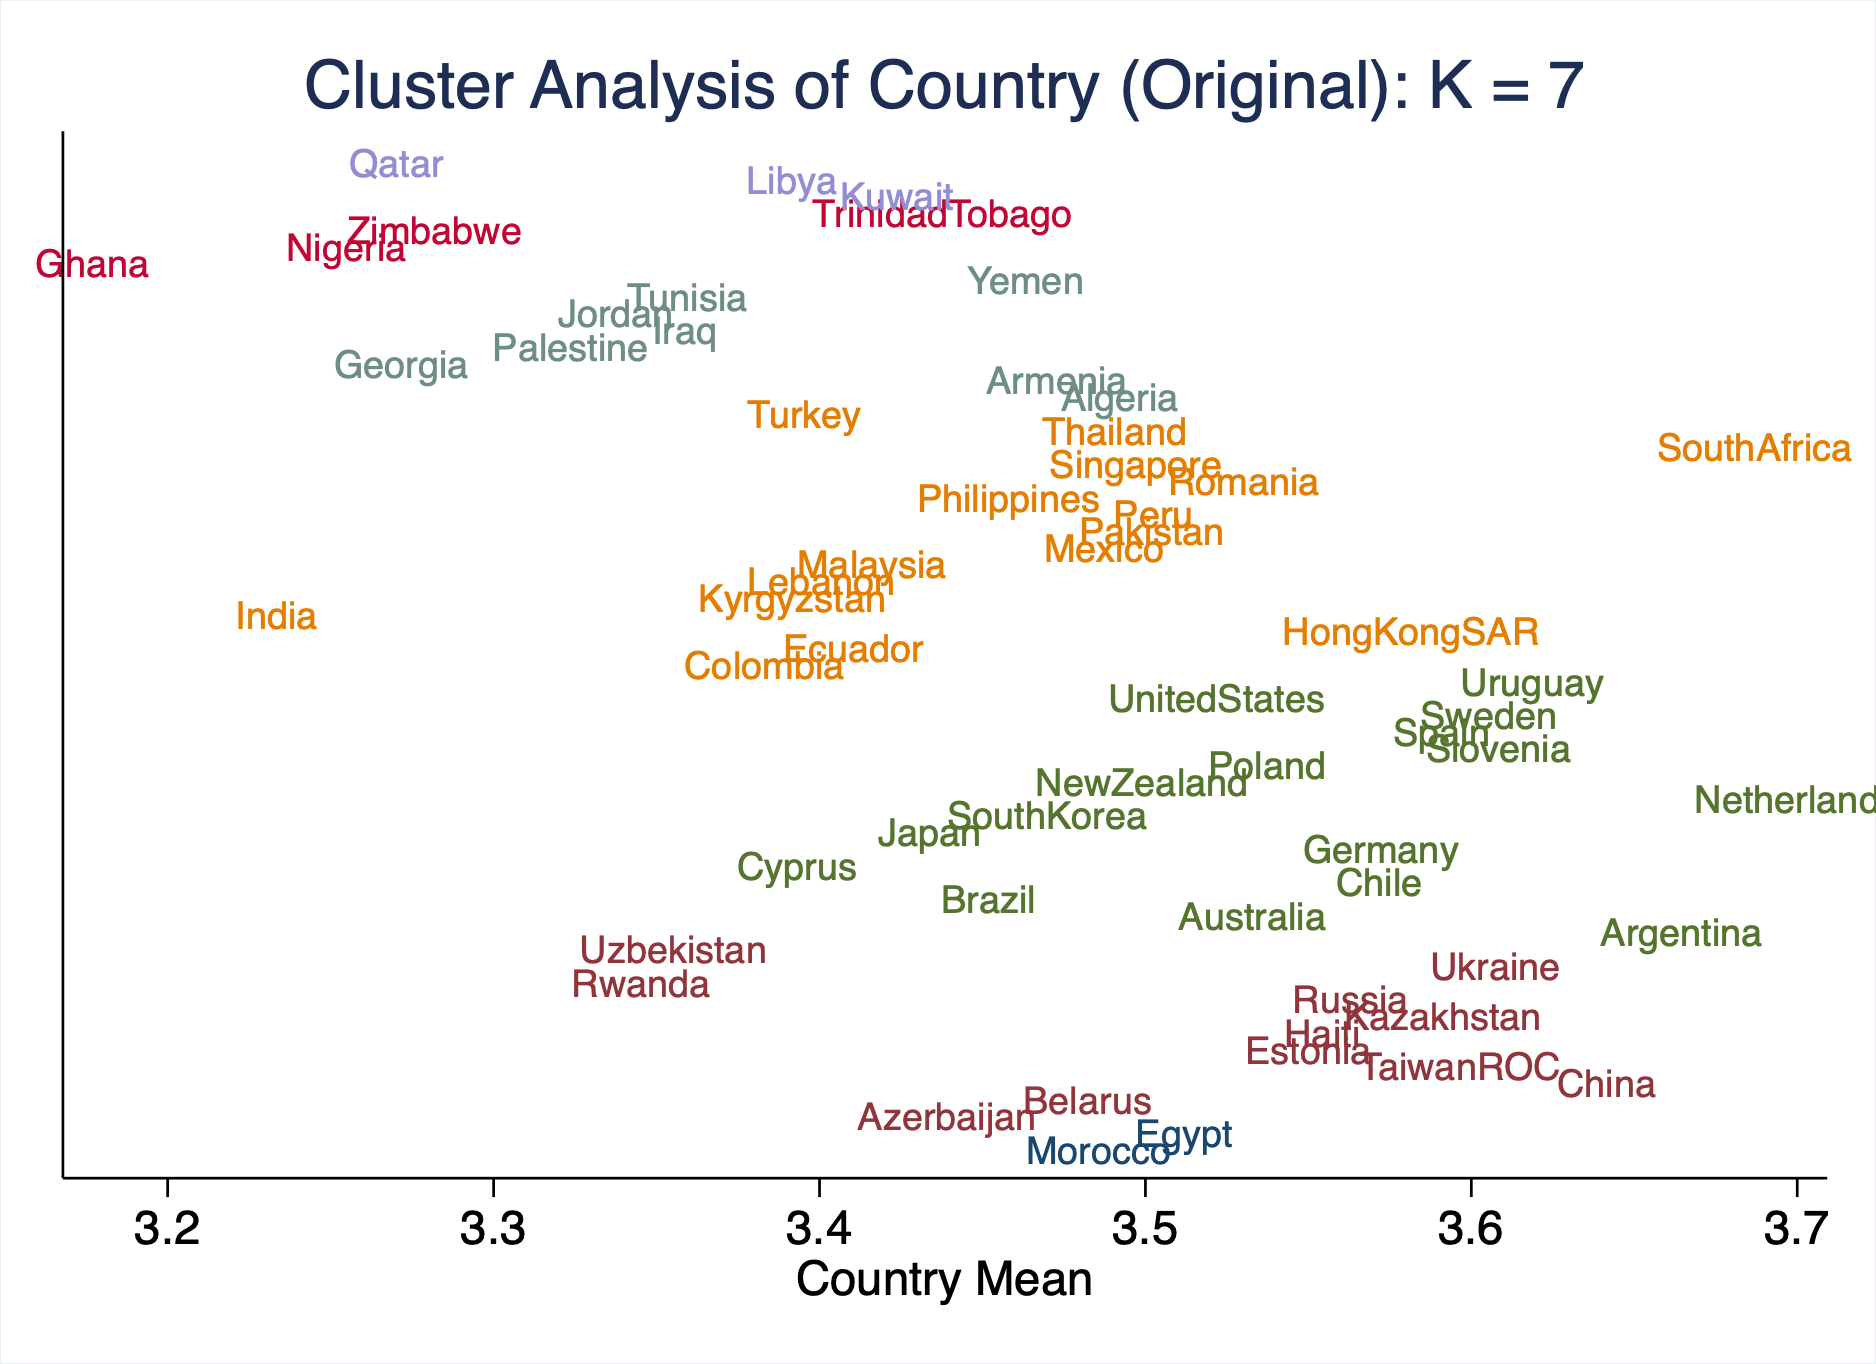
\includegraphics[scale=0.15]{CA_CountryK7_ORI.png}
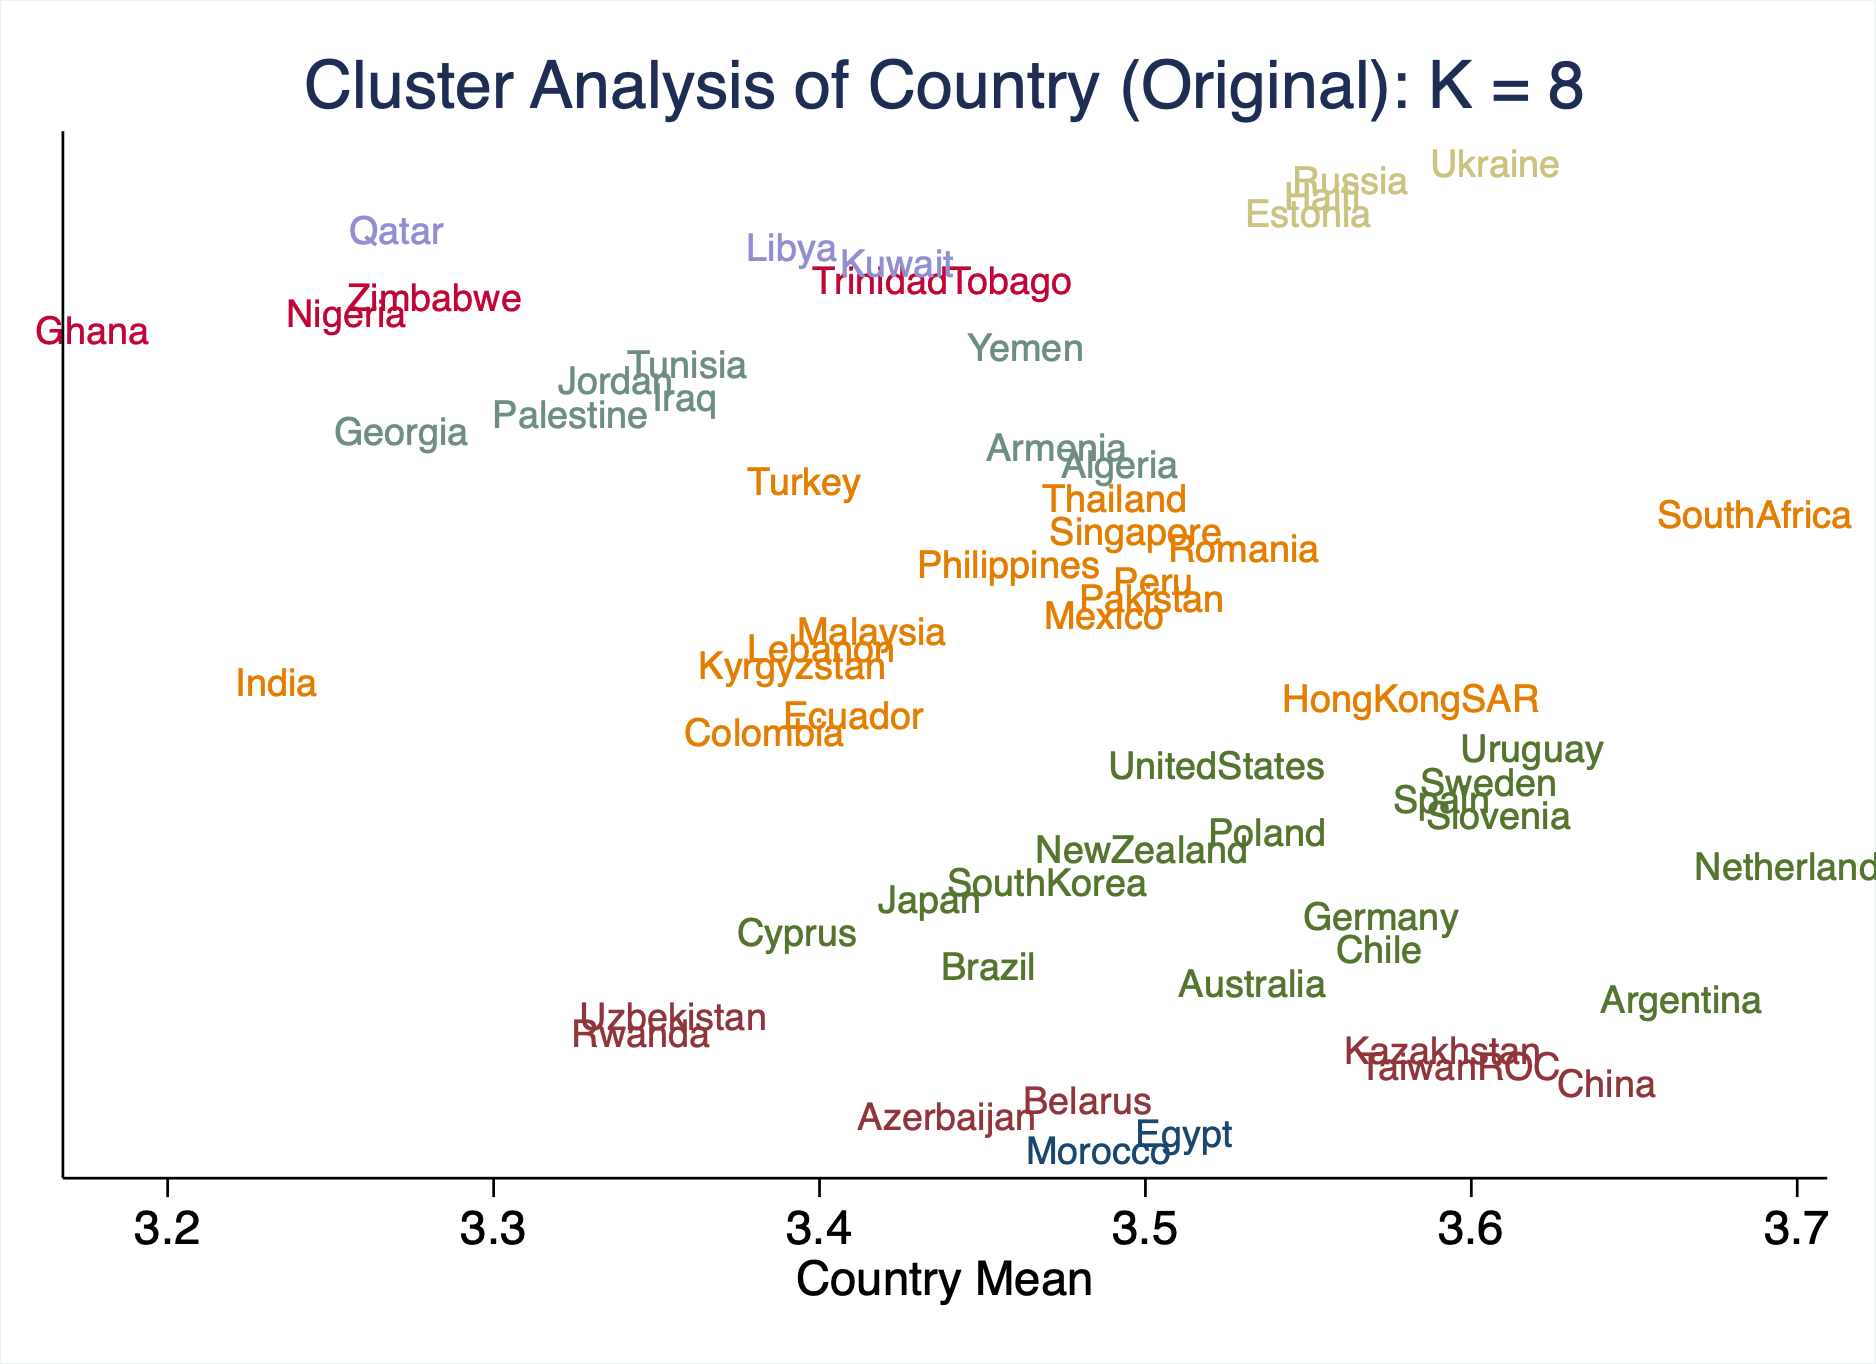
\includegraphics[scale=0.15]{CA_CountryK8_ORI.png}
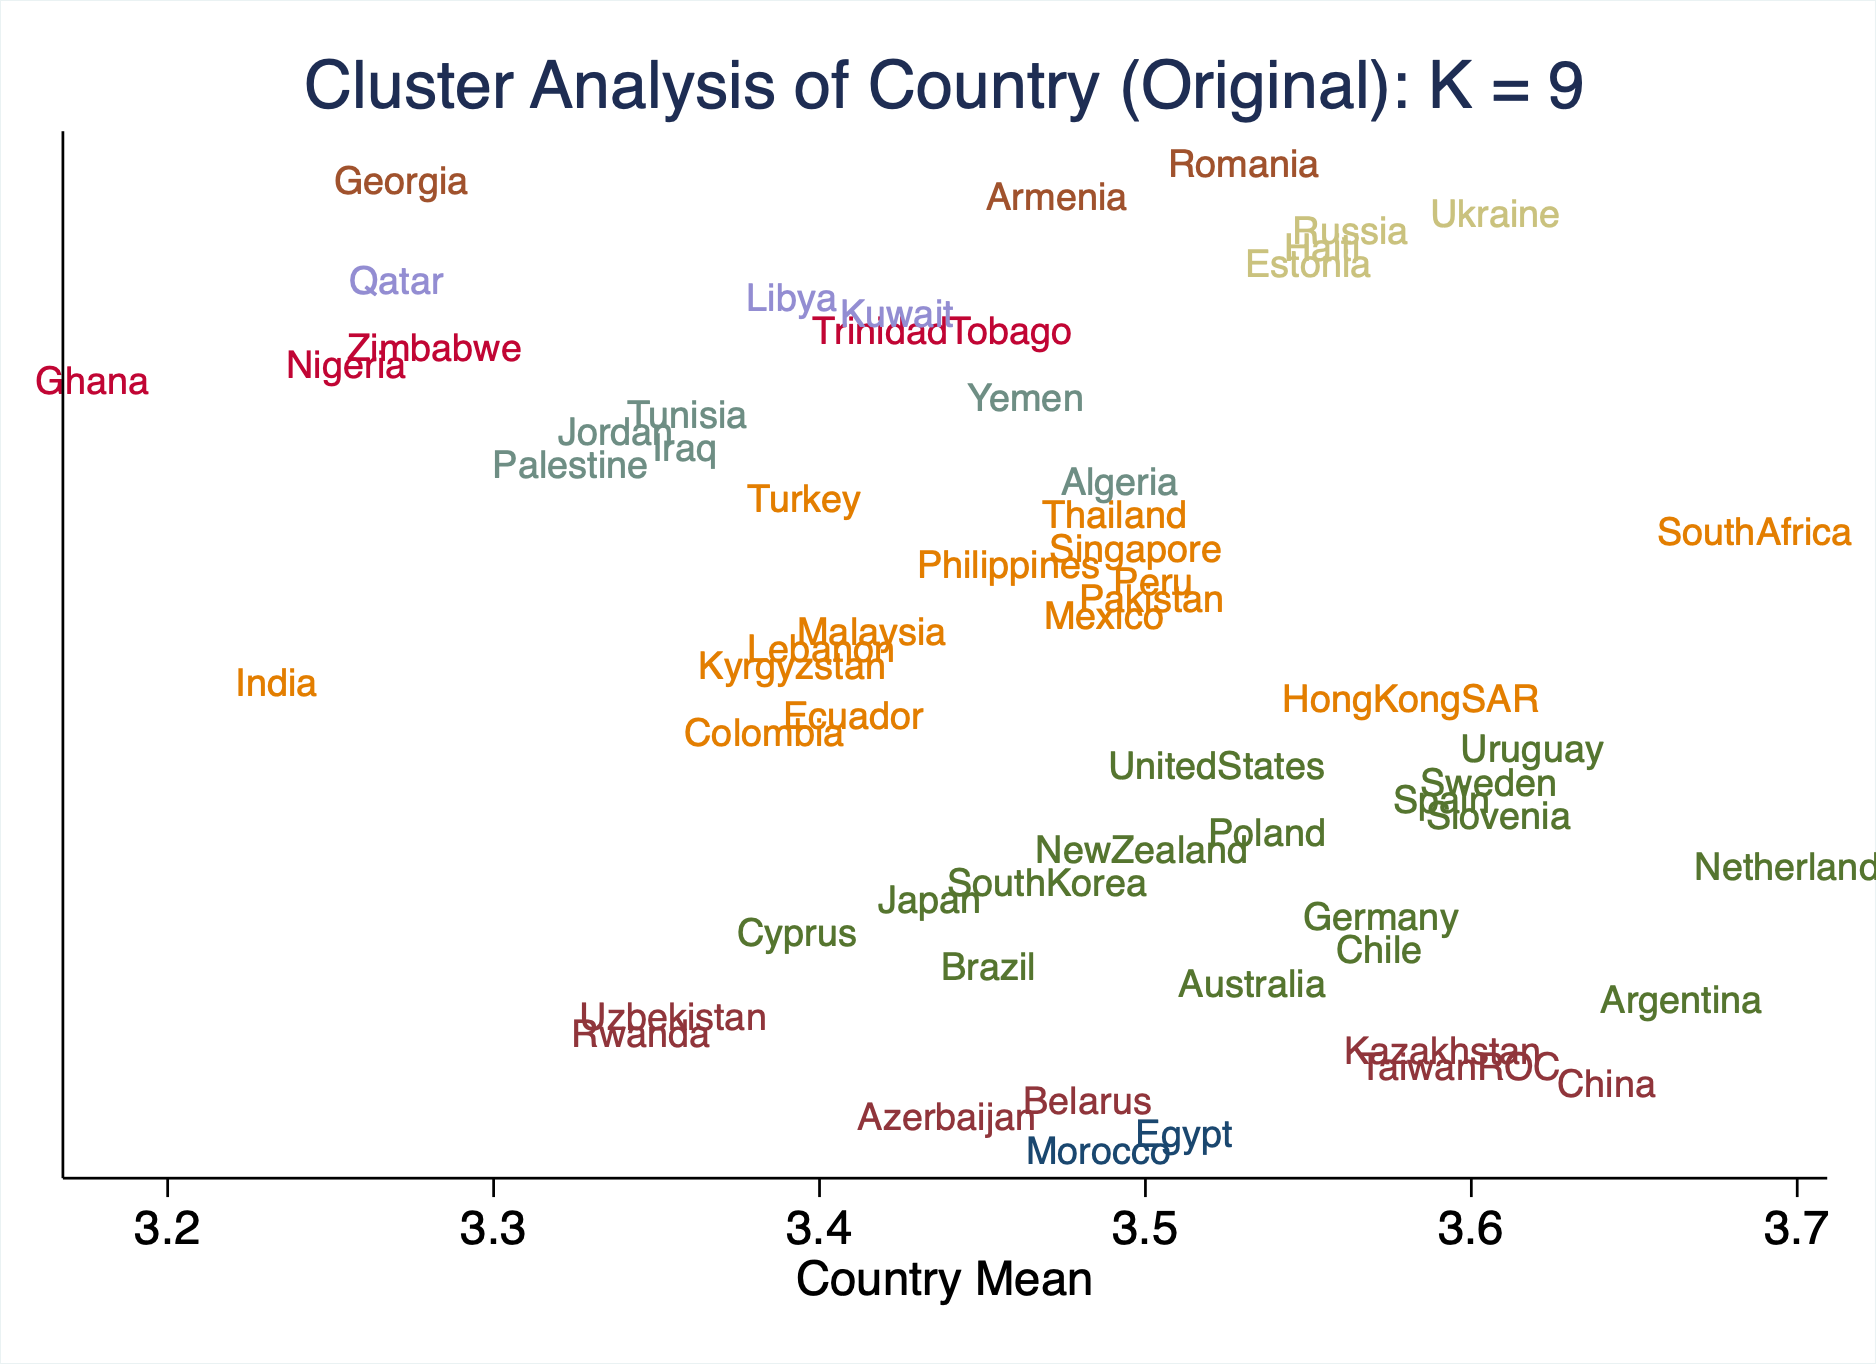
\includegraphics[scale=0.15]{CA_CountryK9_ORI.png}
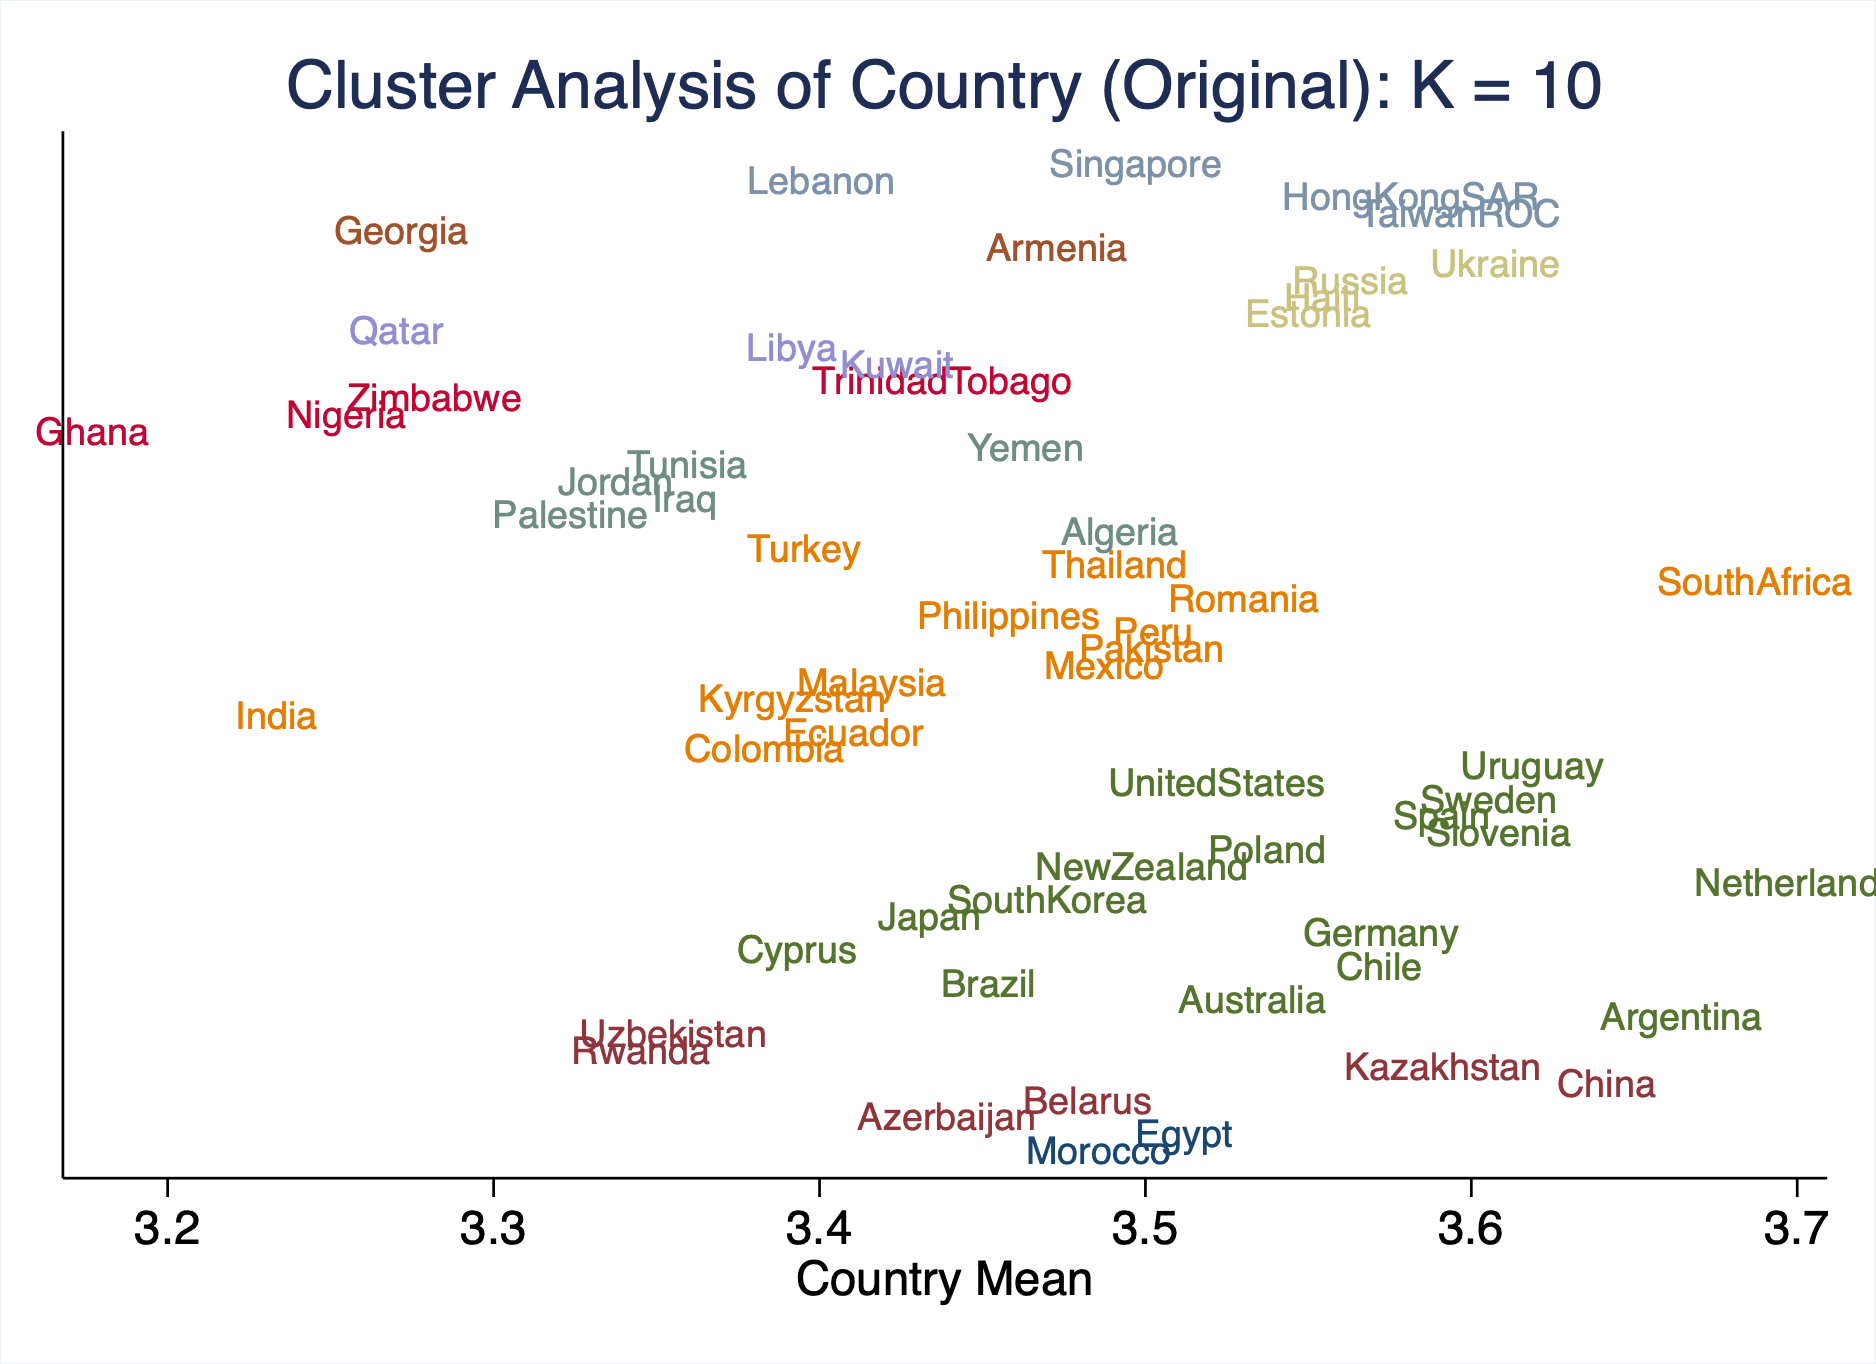
\includegraphics[scale=0.15]{CA_CountryK10_ORI.png}
\end{center}
Similar to the question clustering, figure 3 constitutes the clustering of countries with various numbers of clusters. The preferred number of cluster is five and is shown in figure 4.
\end{figure}  
\begin{figure}  [h!]
\begin{center}
\caption{Cluster analysis of country with non-normalized data (K=5)}
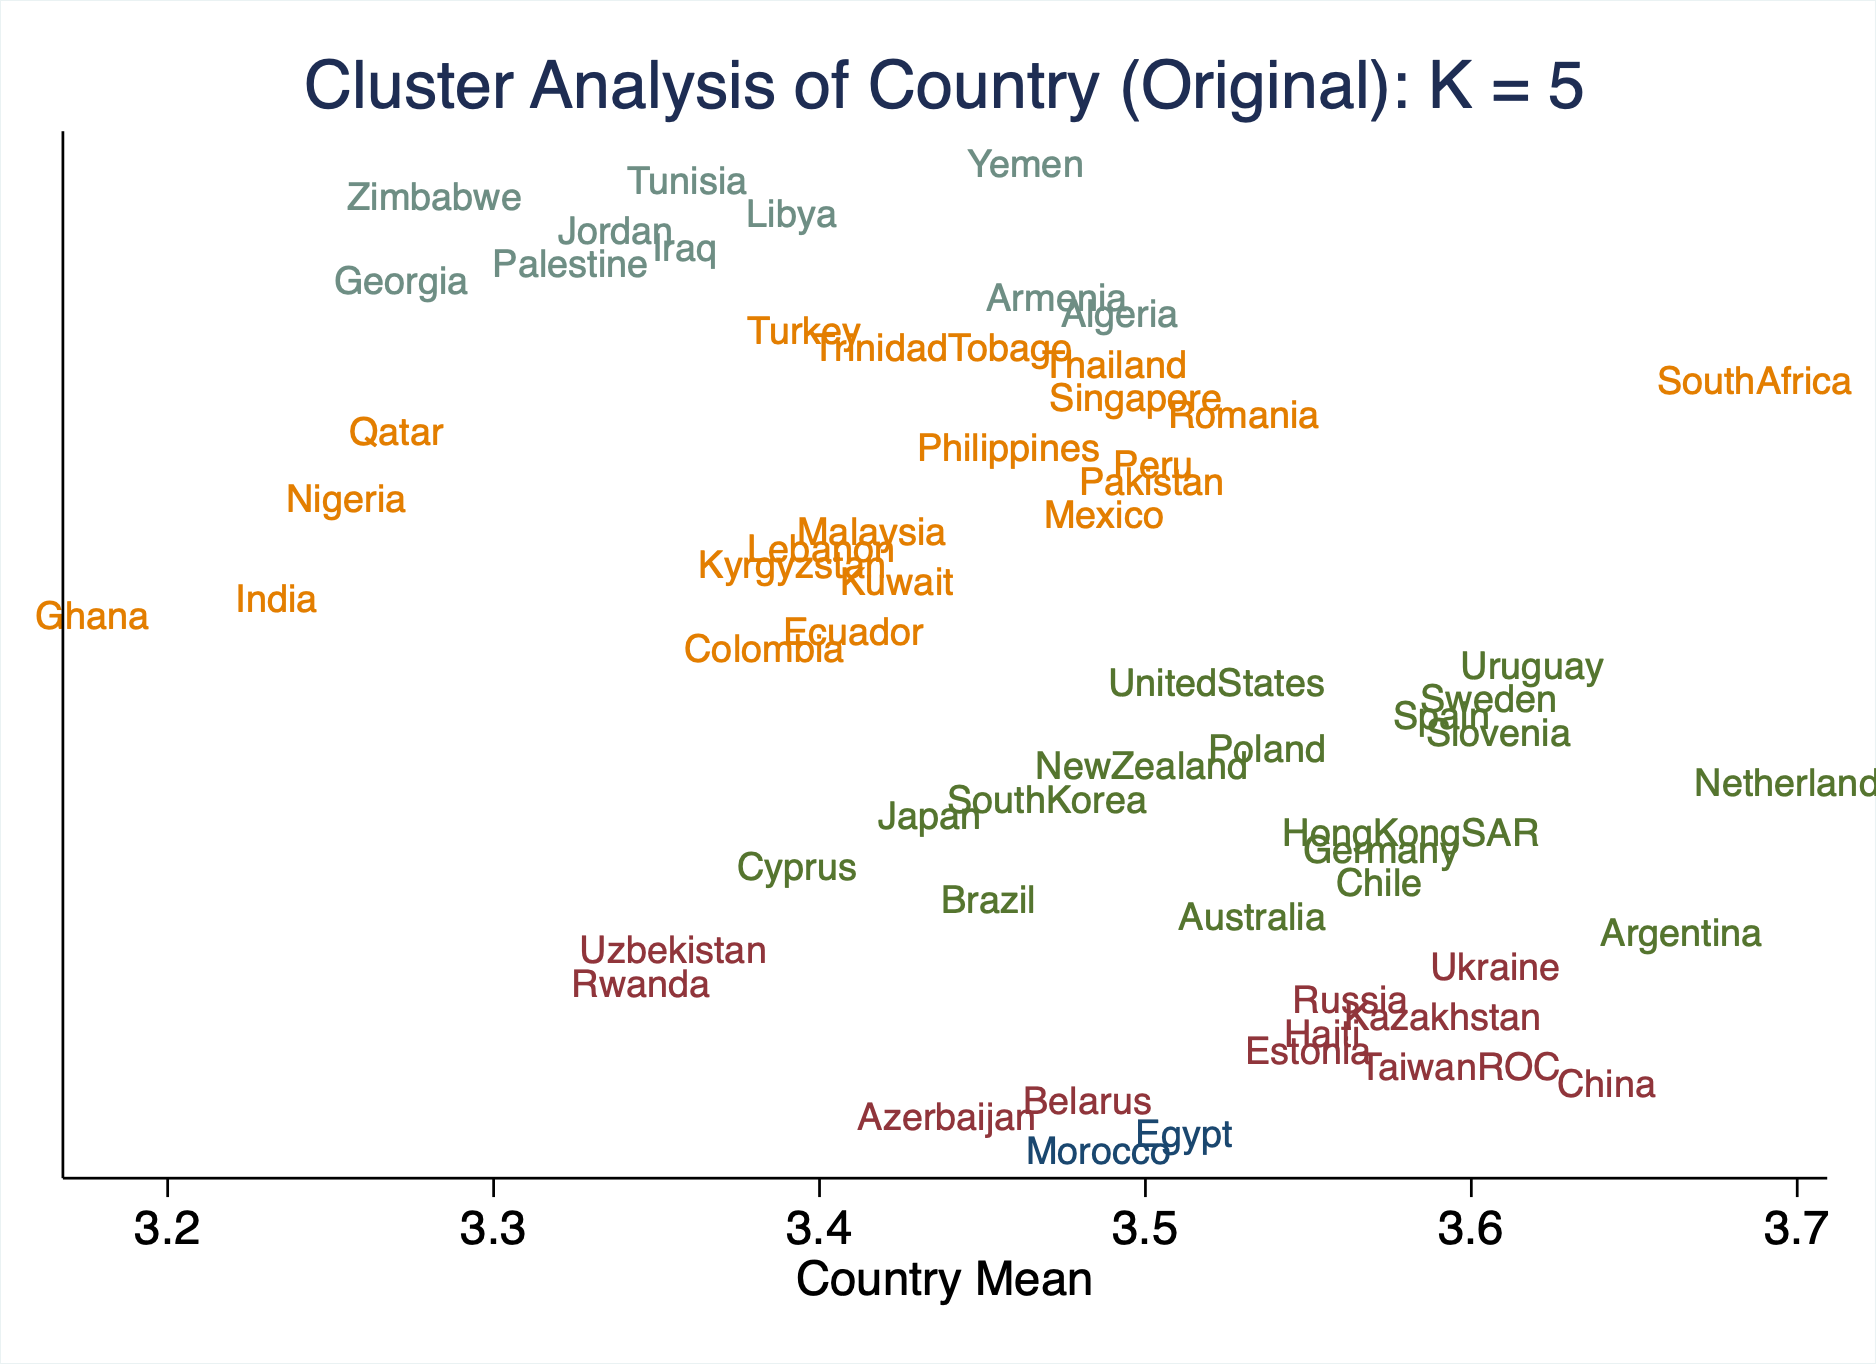
\includegraphics[scale=0.25]{CA_CountryK5_ORI.png}
\end{center}
\end{figure}  

\begin{table}[tbp]
\centering
\caption{List of cluster groups and questions for cluster analysis with K=5}
\begin{adjustbox}{width=0.7\textwidth}
\small
\documentclass{article}
\usepackage{booktabs}
\usepackage{tabularx}
\usepackage[margin=1in]{geometry}
\begin{document}

\begin{table}[tbp] \centering
\newcolumntype{R}{>{\raggedleft\arraybackslash}X}
\newcolumntype{L}{>{\raggedright\arraybackslash}X}
\newcolumntype{C}{>{\centering\arraybackslash}X}

\begin{tabularx}{\linewidth}{@{}lCCC@{}}

\toprule
{Group ID}&{Group}&{Question Code}&{Question} \tabularnewline
\midrule \addlinespace[\belowrulesep]
1&Politics&V110&Confidence: The Press \tabularnewline
1&Politics&V111&Confidence: Television \tabularnewline
1&Politics&V113&Confidence: The Police \tabularnewline
1&Politics&V114&Confidence: Justice System/Courts \tabularnewline
1&Politics&V115&Confidence: The Government \tabularnewline
1&Politics&V117&Confidence: Parliament \tabularnewline
1&Politics&V120&Confidence: Major Companies \tabularnewline
1&Politics&V121&Confidence: Banks \tabularnewline
1&Politics&V122&Confidence: The Environmental Protection Movement \tabularnewline
1&Politics&V123&Confidence: The Women´s Movement \tabularnewline
1&Politics&V126&Confidence: The United Nations \tabularnewline
1&Politics&V155&All religions should be taught in public schools \tabularnewline
1&Politics&V171&Frequency in your neighborhood: Robberies \tabularnewline
1&Politics&V191&Frequency you/family (last 12 month): Gone without a cash income \tabularnewline
1&Politics&V198&Justifiable: Claiming government benefits to which you are not entitled \tabularnewline
1&Politics&V199&Justifiable: Avoiding a fare on public transport \tabularnewline
1&Politics&V209&Justifiable: Parents beating children \tabularnewline
1&Politics&V52&University is more important for a boy than for a girl \tabularnewline
1&Politics&V7&Important in life: Politics \tabularnewline
1&Politics&V70&Schwartz: It is important to this person to think up new ideas and be creative \tabularnewline
1&Politics&V73&Schwartz: It is important to this person to have a good time \tabularnewline
1&Politics&V75&Schwartz: It is important to this person being very successful \tabularnewline
1&Politics&V78&Schwartz: It is important to this person looking after the environment \tabularnewline
2&Life security&V100&Hard work brings success \tabularnewline
2&Life security&V132&Democracy: Religious authorities interpret the laws. \tabularnewline
2&Life security&V173&Frequency in your neighborhood: Police or military interfere with people’s pri \tabularnewline
2&Life security&V174&Frequency in your neighborhood: Racist behavior \tabularnewline
2&Life security&V188&Frequency you/family (last 12 month): Gone without enough food to eat \tabularnewline
2&Life security&V189&Frequency you/family (last 12 month): Felt unsafe from crime in your own home \tabularnewline
2&Life security&V190&Frequency you/family (last 12 month): Gone without needed medicine or treatment  \tabularnewline
2&Life security&V196&It is not important for me to know about science in my daily life \tabularnewline
2&Life security&V205&Justifiable: Divorce \tabularnewline
2&Life security&V71&Schwartz: It is important to this person to be rich \tabularnewline
2&Life security&V76&Schwartz: It is important to this person adventure and taking risks \tabularnewline
2&Life security&V98&Government responsibility \tabularnewline
2&Life security&V99&Competition good or harmful \tabularnewline
3&Life importance&V10&Feeling of happiness \tabularnewline
3&Life importance&V170&Secure in neighborhood \tabularnewline
3&Life importance&V200&Justifiable: Stealing property \tabularnewline
3&Life importance&V202&Justifiable: Someone accepting a bribe \tabularnewline
3&Life importance&V208&Justifiable: For a man to beat his wife \tabularnewline
3&Life importance&V210&Justifiable: Violence against other people \tabularnewline
3&Life importance&V4&Important in life: Family \tabularnewline
3&Life importance&V49&One of main goals in life has been to make my parents proud \tabularnewline
3&Life importance&V5&Important in life: Friends \tabularnewline
3&Life importance&V6&Important in life: Leisure time \tabularnewline
3&Life importance&V8&Important in life: Work \tabularnewline
4&Democracy and freedom&V101&Wealth accumulation \tabularnewline
4&Democracy and freedom&V131&Democracy: Governments tax the rich and subsidize the poor. \tabularnewline
4&Democracy and freedom&V133&Democracy: People choose their leaders in free elections. \tabularnewline
4&Democracy and freedom&V134&Democracy: People receive state aid for unemployment. \tabularnewline
4&Democracy and freedom&V136&Democracy: Civil rights protect people’s liberty against oppression. \tabularnewline
4&Democracy and freedom&V137&Democracy: The state makes people's incomes equal \tabularnewline
4&Democracy and freedom&V138&Democracy: People obey their rulers \tabularnewline
4&Democracy and freedom&V139&Democracy: Women have the same rights as men. \tabularnewline
4&Democracy and freedom&V192&Science and technology are making our lives healthier, easier, and more comforta \tabularnewline
4&Democracy and freedom&V193&Because of science and technology, there will be more opportunities for the next \tabularnewline
4&Democracy and freedom&V194&We depend too much on science and not enough on faith \tabularnewline
4&Democracy and freedom&V195&One of the bad effects of science is that it breaks down people’s ideas of rig \tabularnewline
4&Democracy and freedom&V197&The world is better off, or worse off, because of science and technology \tabularnewline
4&Democracy and freedom&V55&How much freedom of choice and control \tabularnewline
4&Democracy and freedom&V59&Satisfaction with financial situation of household \tabularnewline
4&Democracy and freedom&V96&Income equality \tabularnewline
4&Democracy and freedom&V97&Private vs state ownership of business \tabularnewline
5&Traditional values&V108&Confidence: Churches \tabularnewline
5&Traditional values&V11&State of health (subjective) \tabularnewline
5&Traditional values&V119&Confidence: Universities \tabularnewline
5&Traditional values&V124&Confidence: Charitable or humanitarian organizations \tabularnewline
5&Traditional values&V153&Whenever science and religion conflict,  religion is always right \tabularnewline
5&Traditional values&V156&People who belong to different religions are probably just as moral as those who \tabularnewline
5&Traditional values&V181&Worries: Losing my job or not finding a job \tabularnewline
5&Traditional values&V182&Worries: Not being able to give one's children a good education \tabularnewline
5&Traditional values&V183&Worries: A war involving my country \tabularnewline
5&Traditional values&V184&Worries: A terrorist attack \tabularnewline
5&Traditional values&V207&Justifiable: Suicide \tabularnewline
5&Traditional values&V51&Men make better political leaders than women do \tabularnewline
5&Traditional values&V53&Men make better business executives than women do \tabularnewline
5&Traditional values&V54&Being a housewife just as fulfilling \tabularnewline
5&Traditional values&V72&Schwartz: It is important to this person living in secure surroundings \tabularnewline
5&Traditional values&V77&Schwartz: It is important to this person to always behave properly \tabularnewline
5&Traditional values&V79&Schwartz: It is important to this person tradition \tabularnewline
5&Traditional values&V9&Important in life: Religion \tabularnewline
\bottomrule 

\end{tabularx}
\end{table}
\end{document}

\end{adjustbox}
\end{table}


\pagebreak
\begin{figure}  [h!]
\subsection{Normalized data}
\subsubsection{Question clustering}
\begin{center}
\caption{Cluster analysis of questions with normalized data}
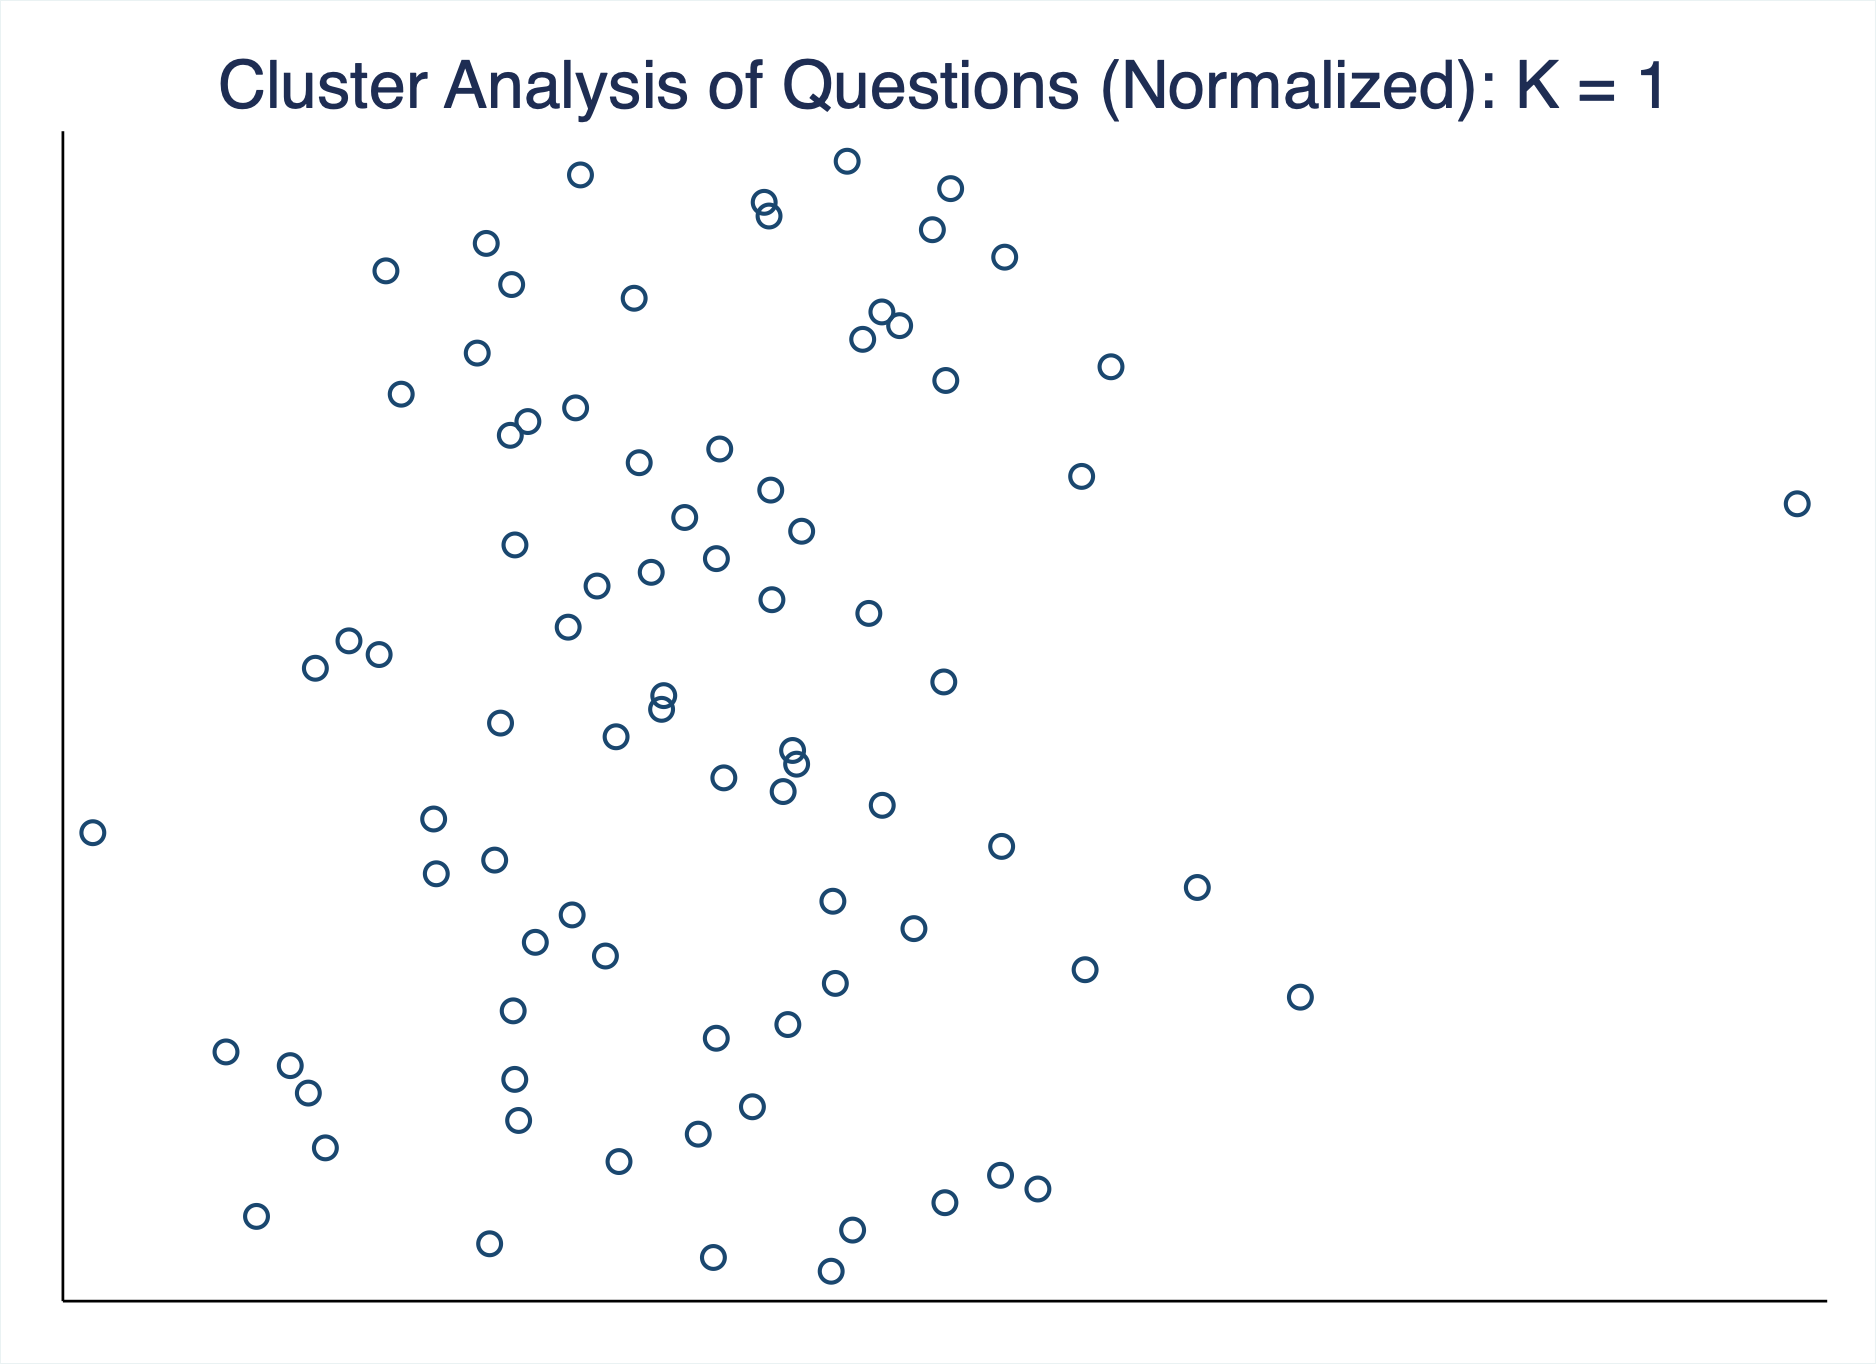
\includegraphics[scale=0.15]{CA_QuestionK1_NOR.png}
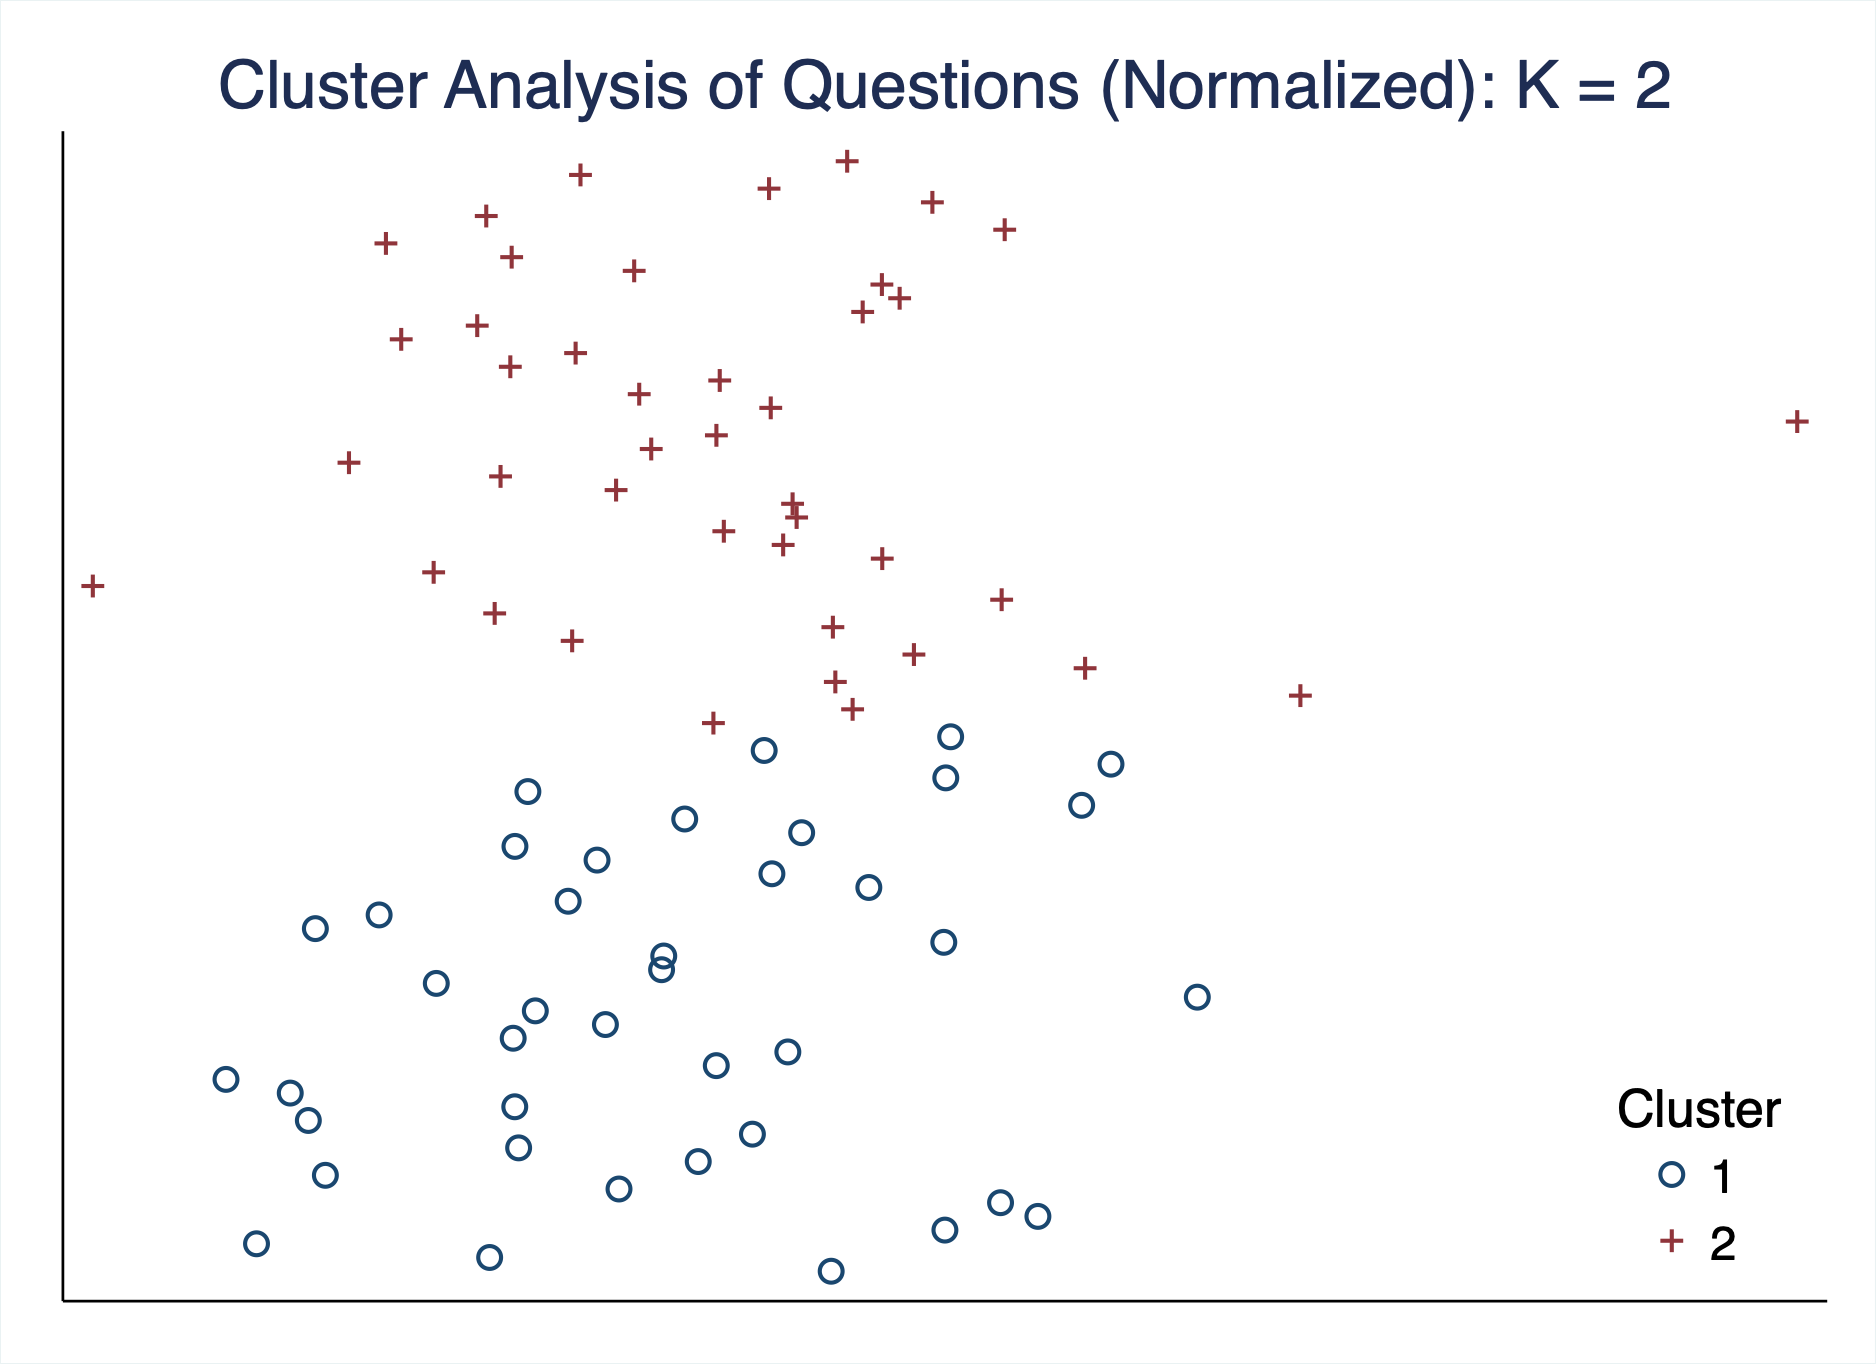
\includegraphics[scale=0.15]{CA_QuestionK2_NOR.png}
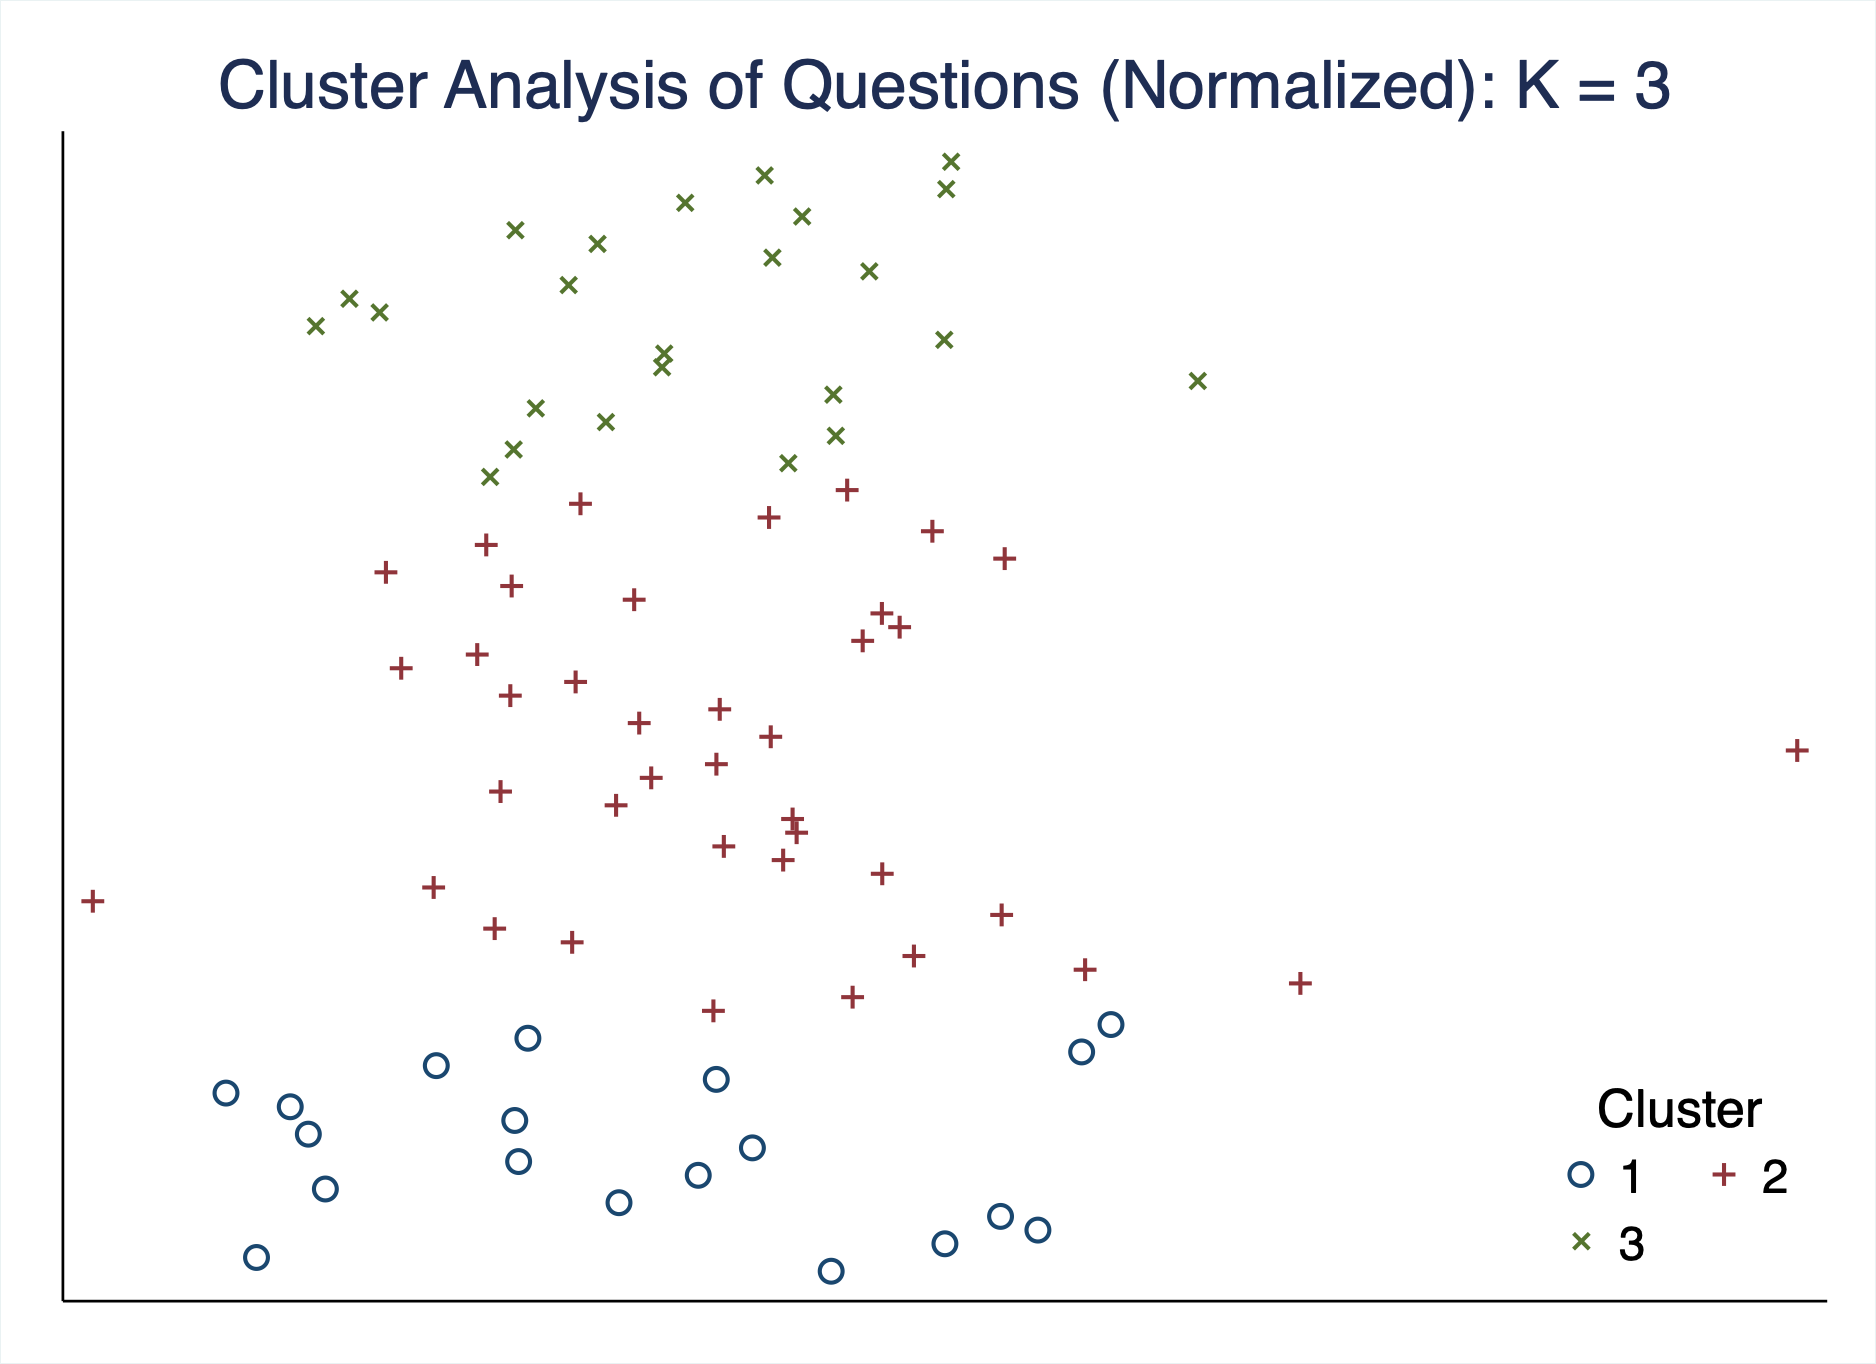
\includegraphics[scale=0.15]{CA_QuestionK3_NOR.png}
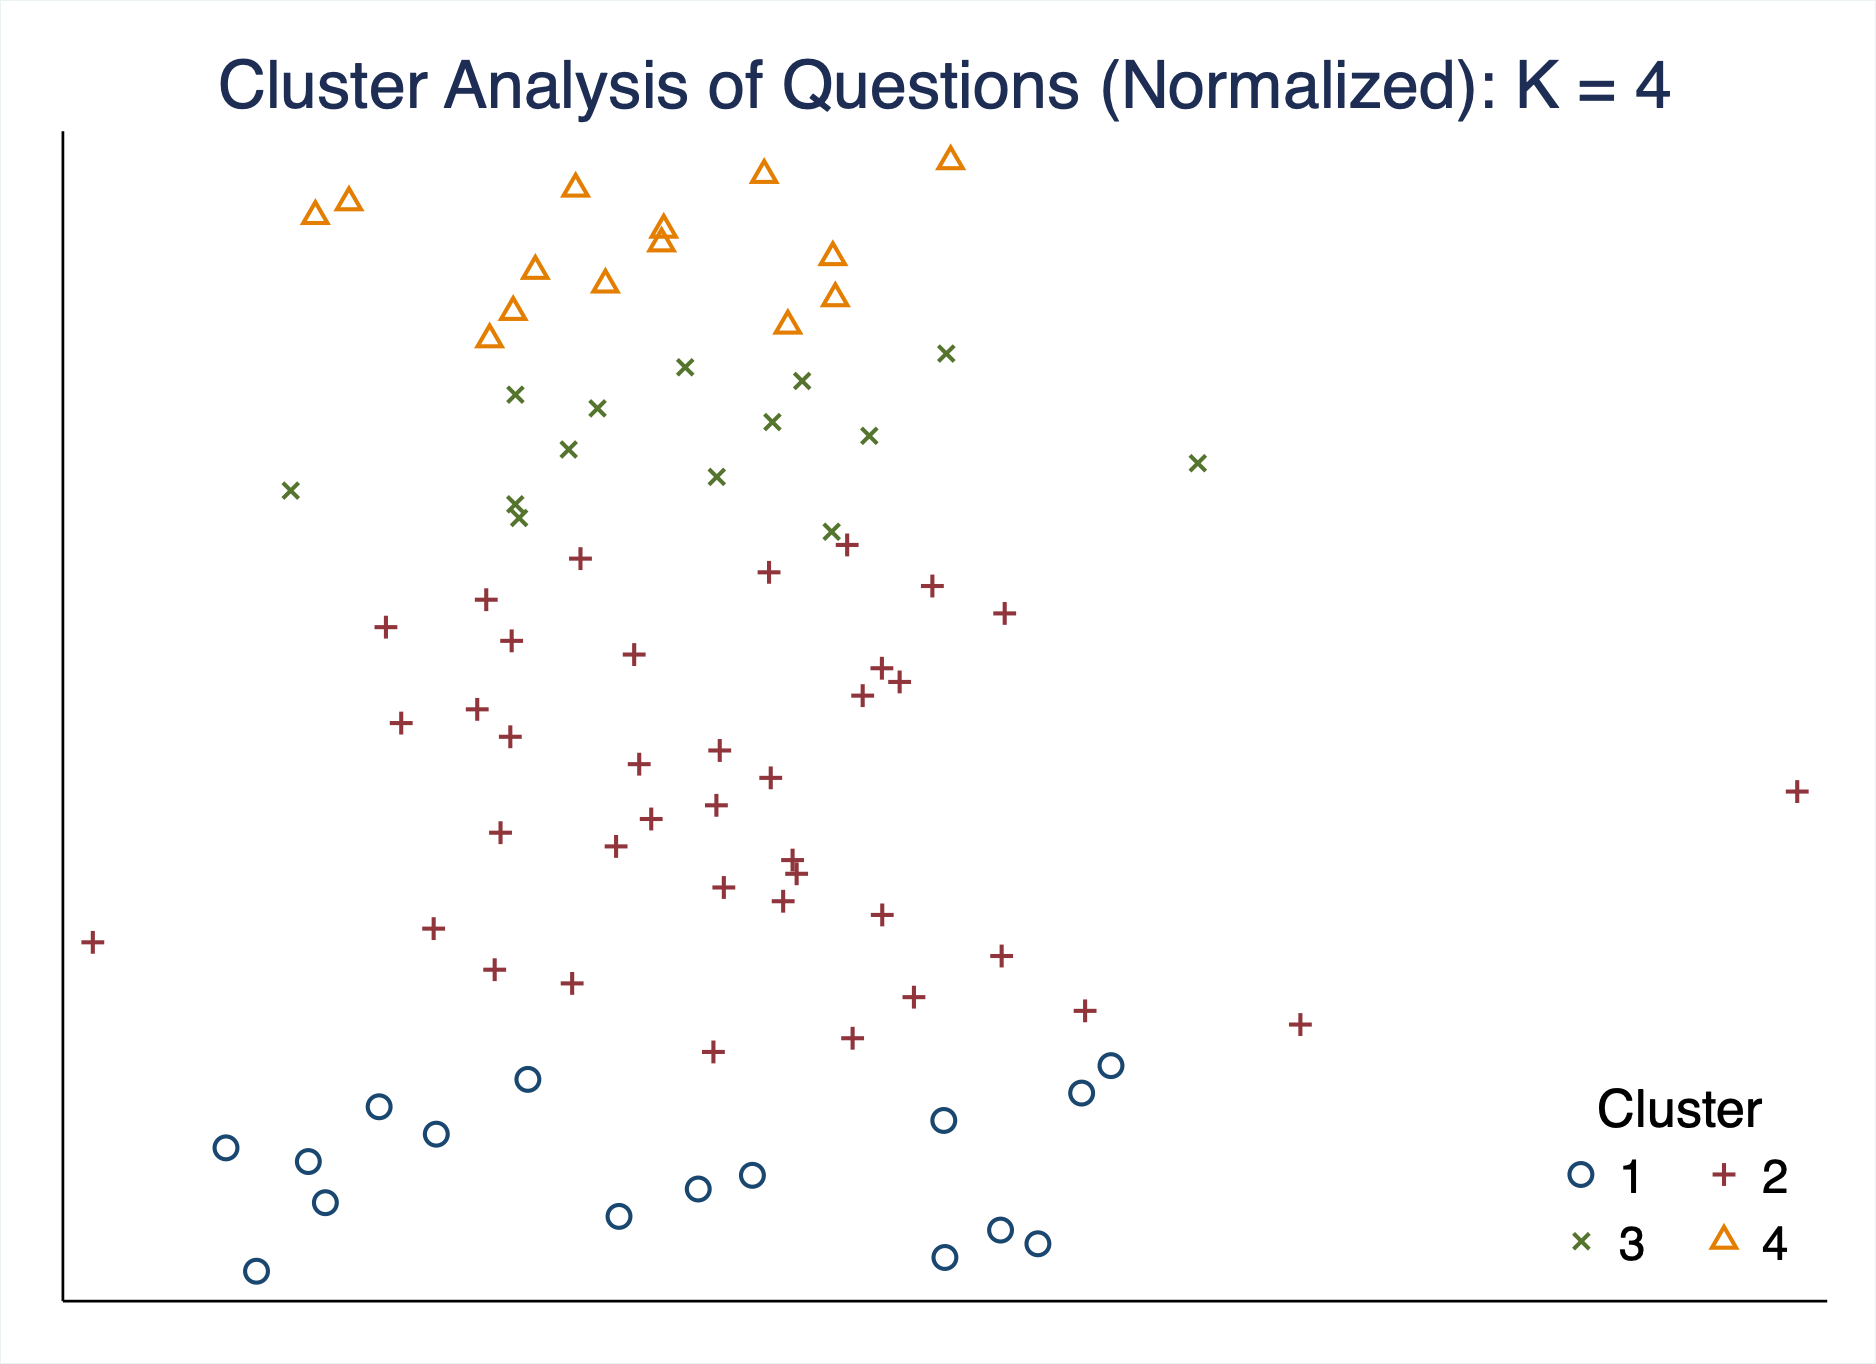
\includegraphics[scale=0.15]{CA_QuestionK4_NOR.png}
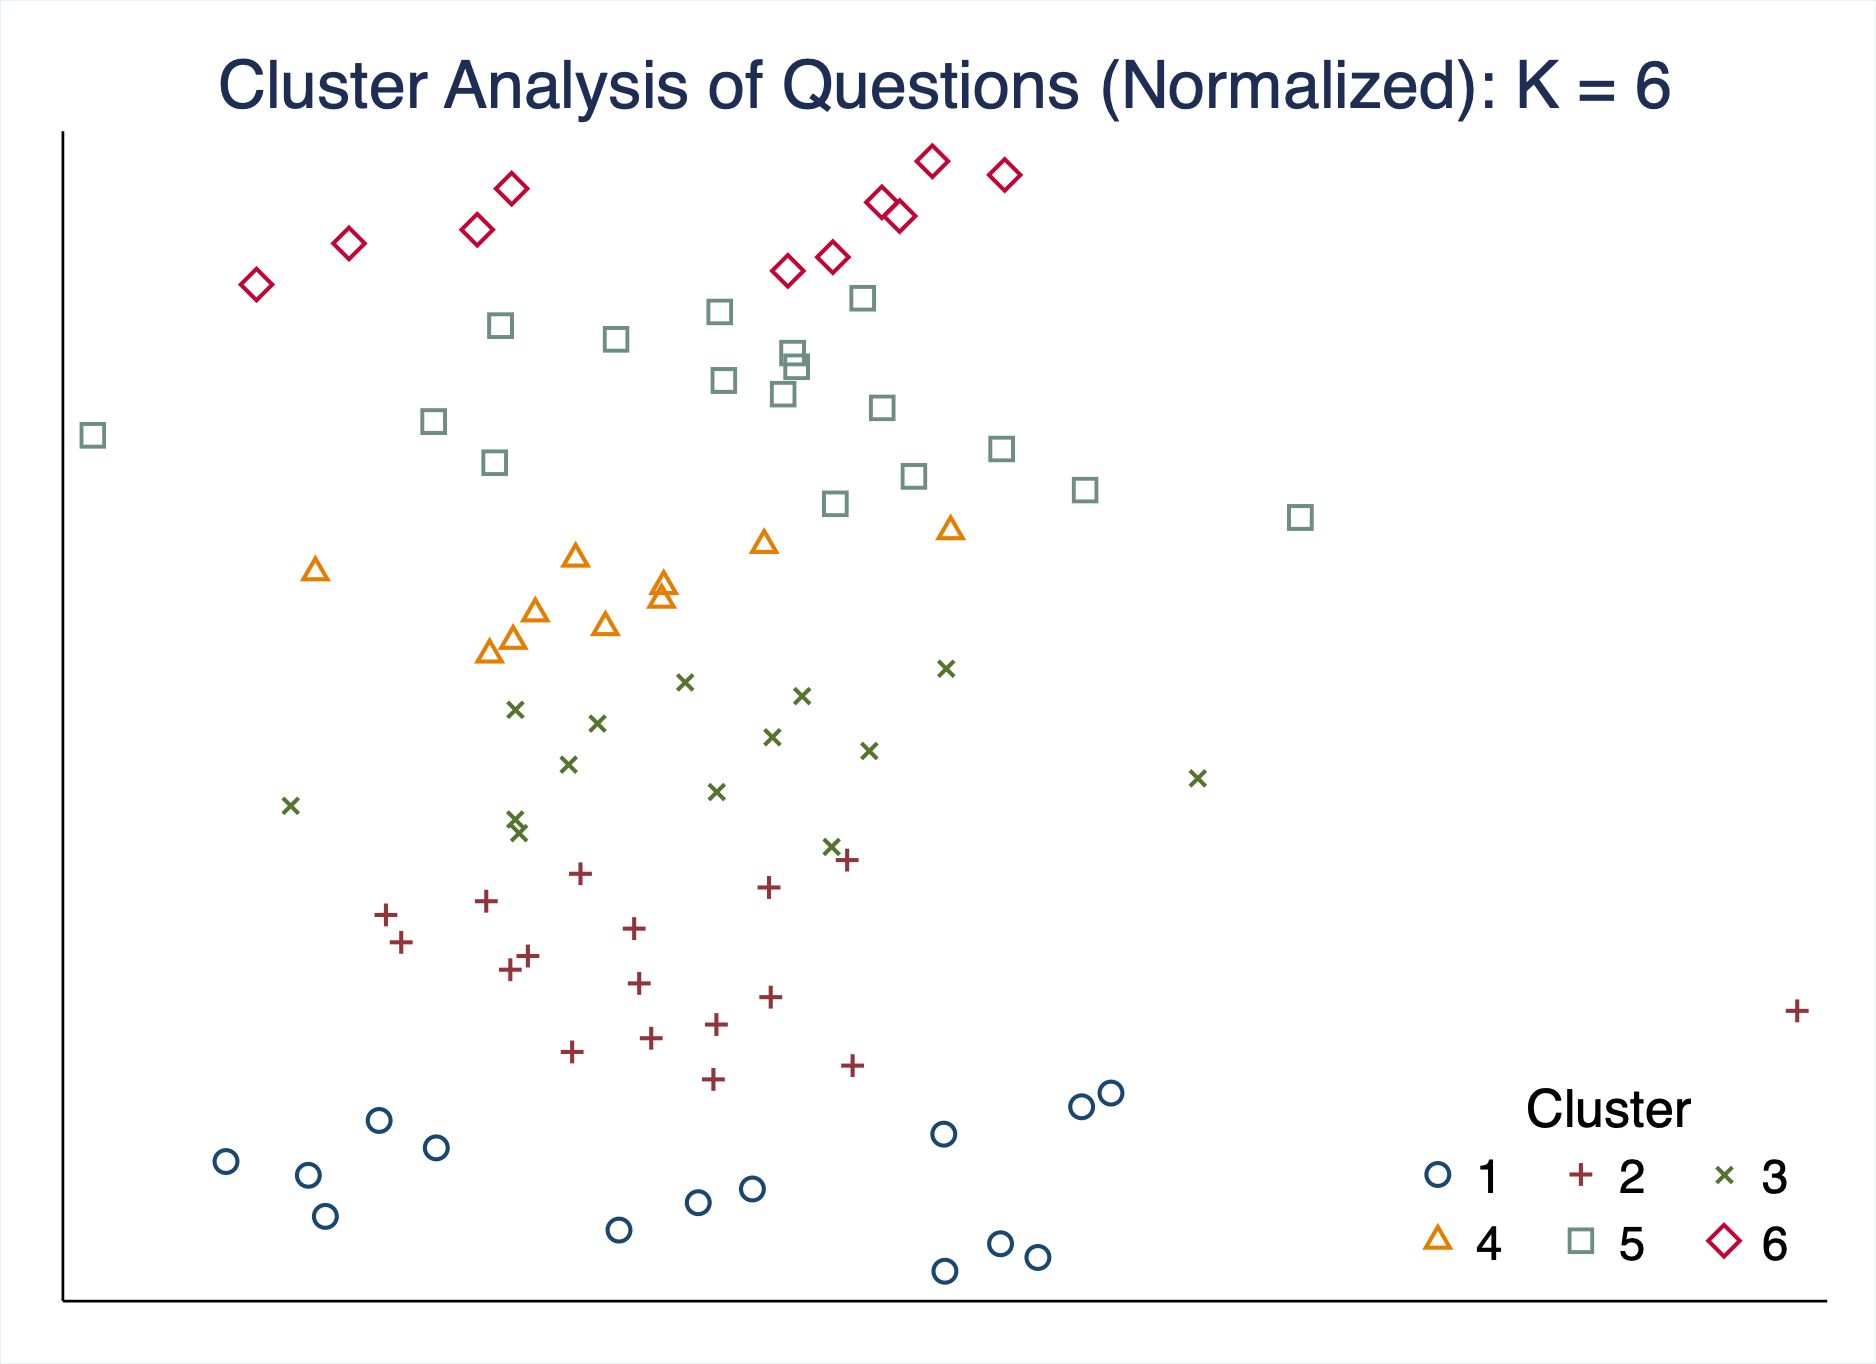
\includegraphics[scale=0.15]{CA_QuestionK6_NOR.png}
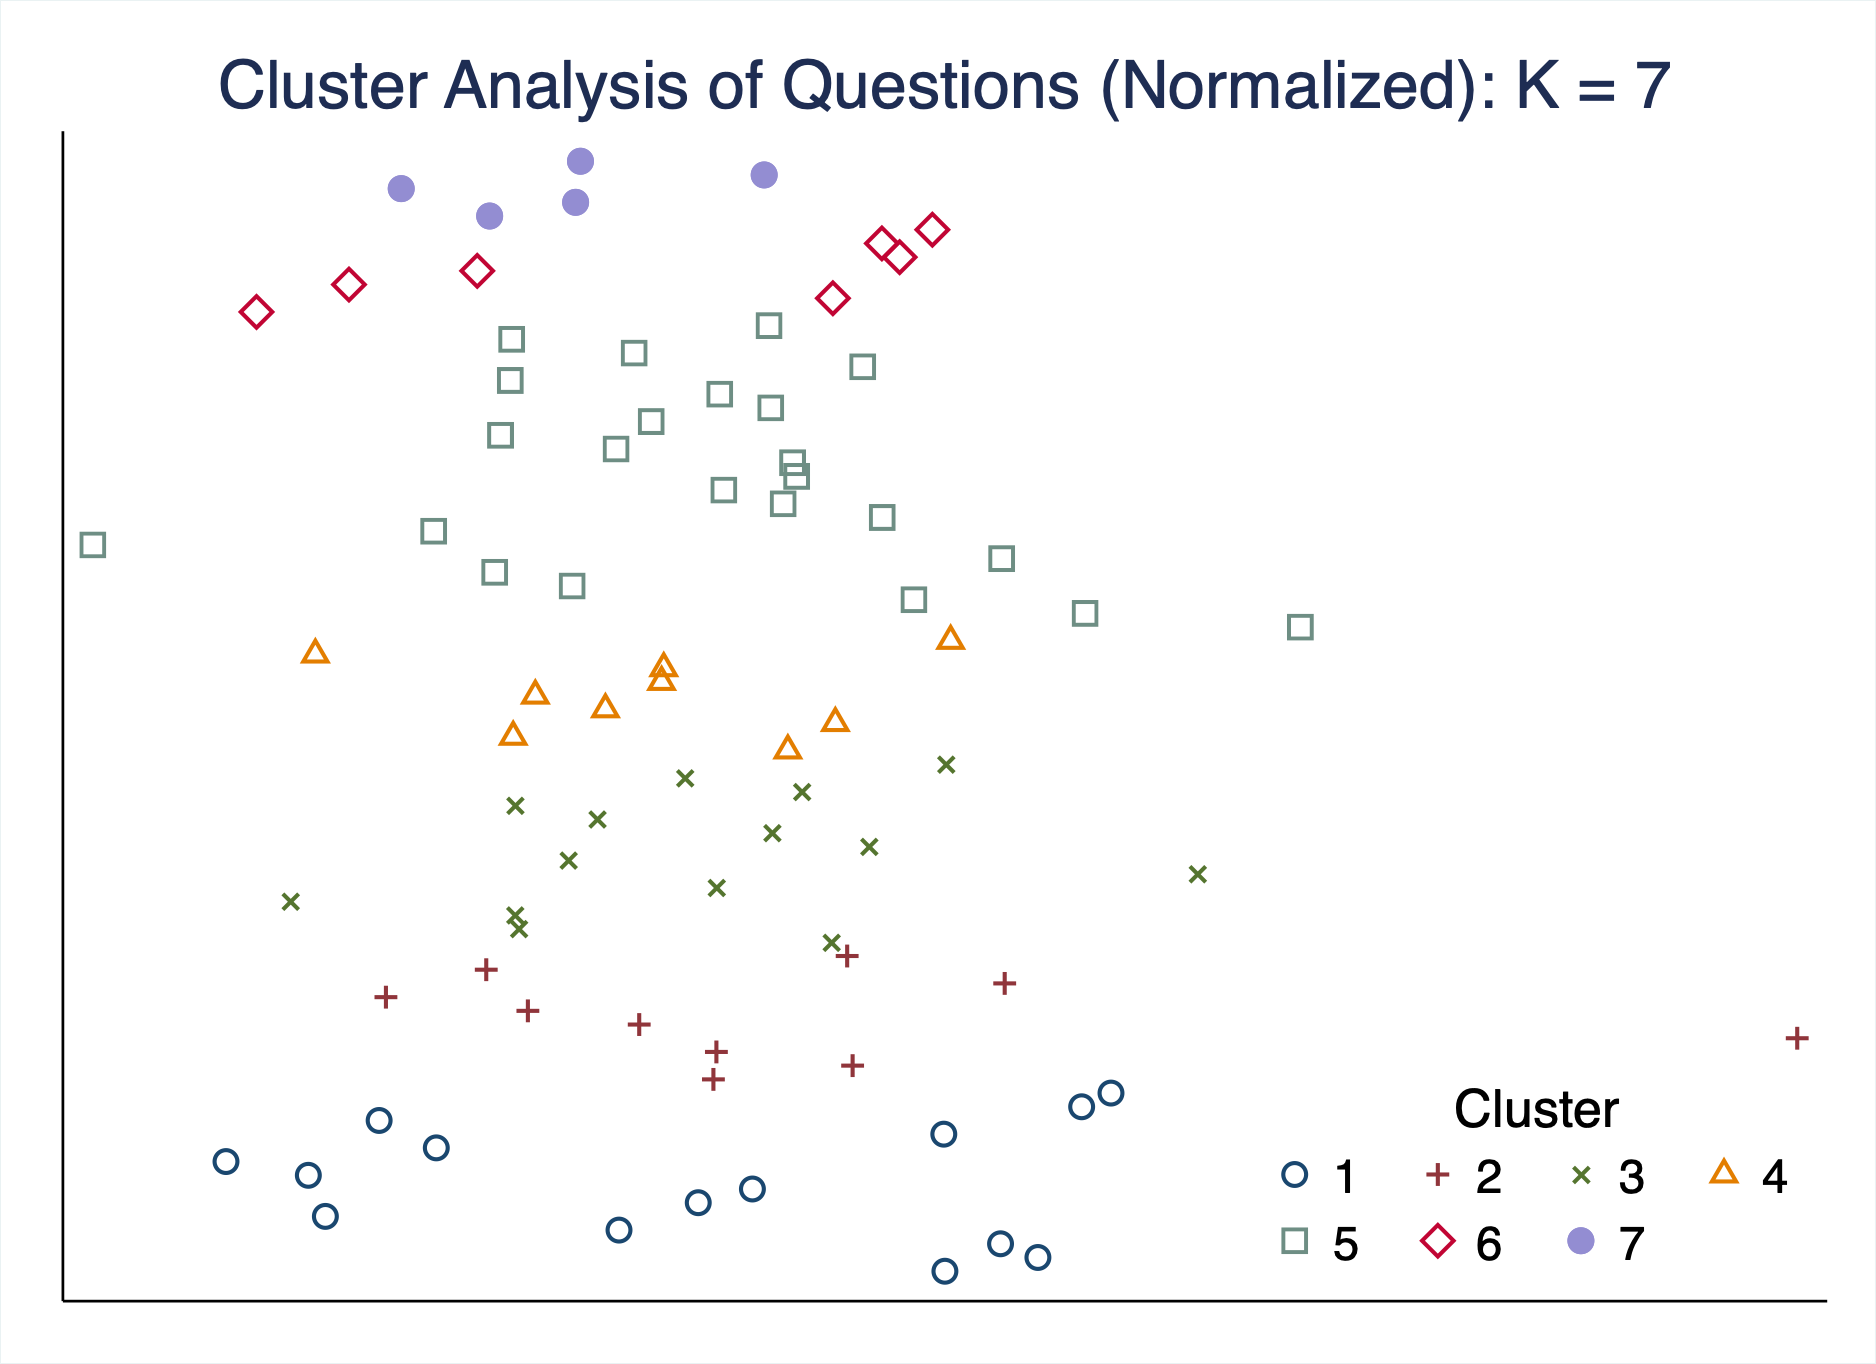
\includegraphics[scale=0.15]{CA_QuestionK7_NOR.png}
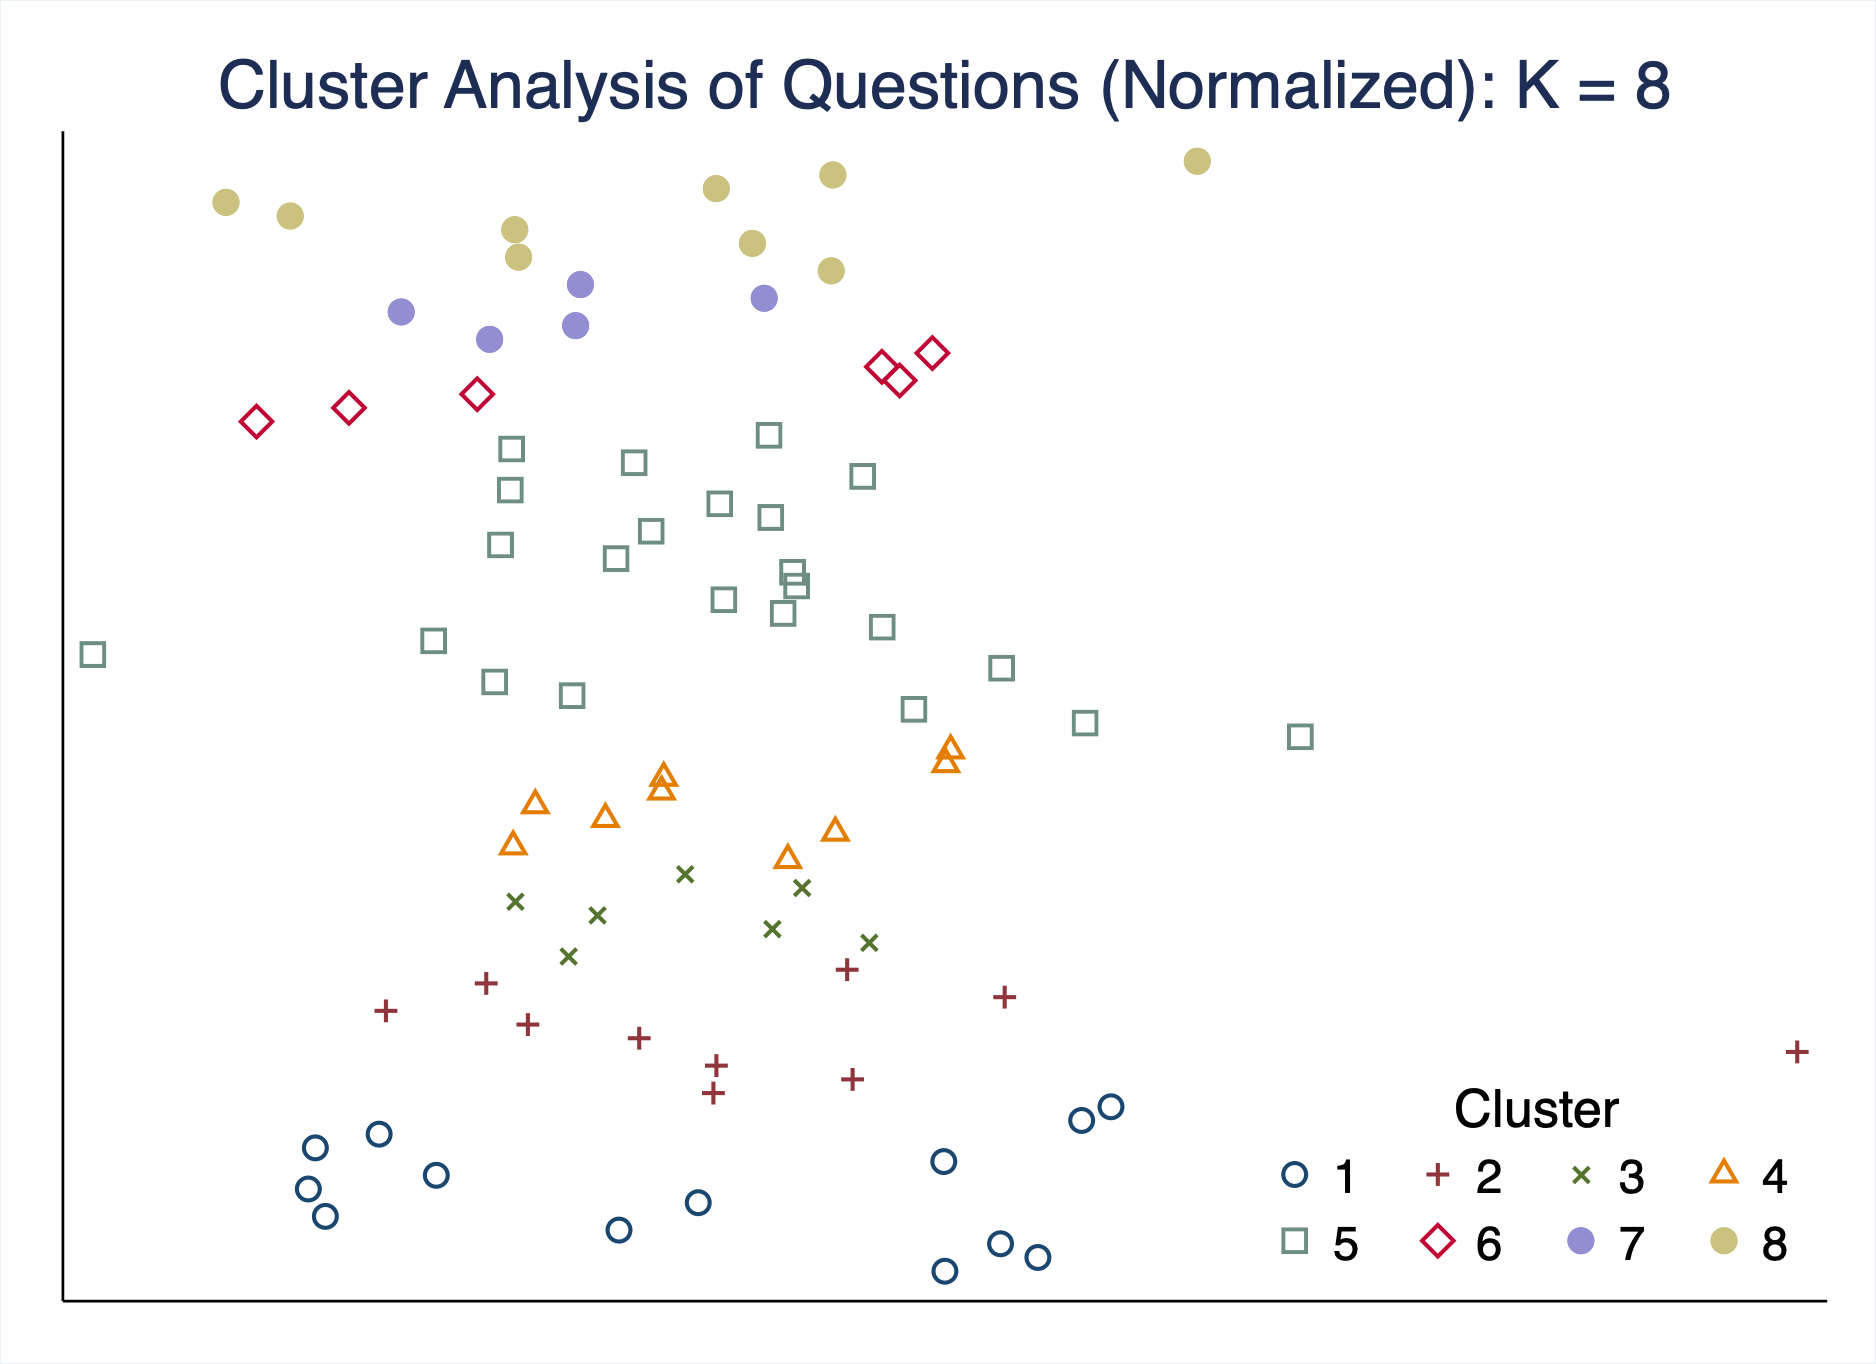
\includegraphics[scale=0.15]{CA_QuestionK8_NOR.png}
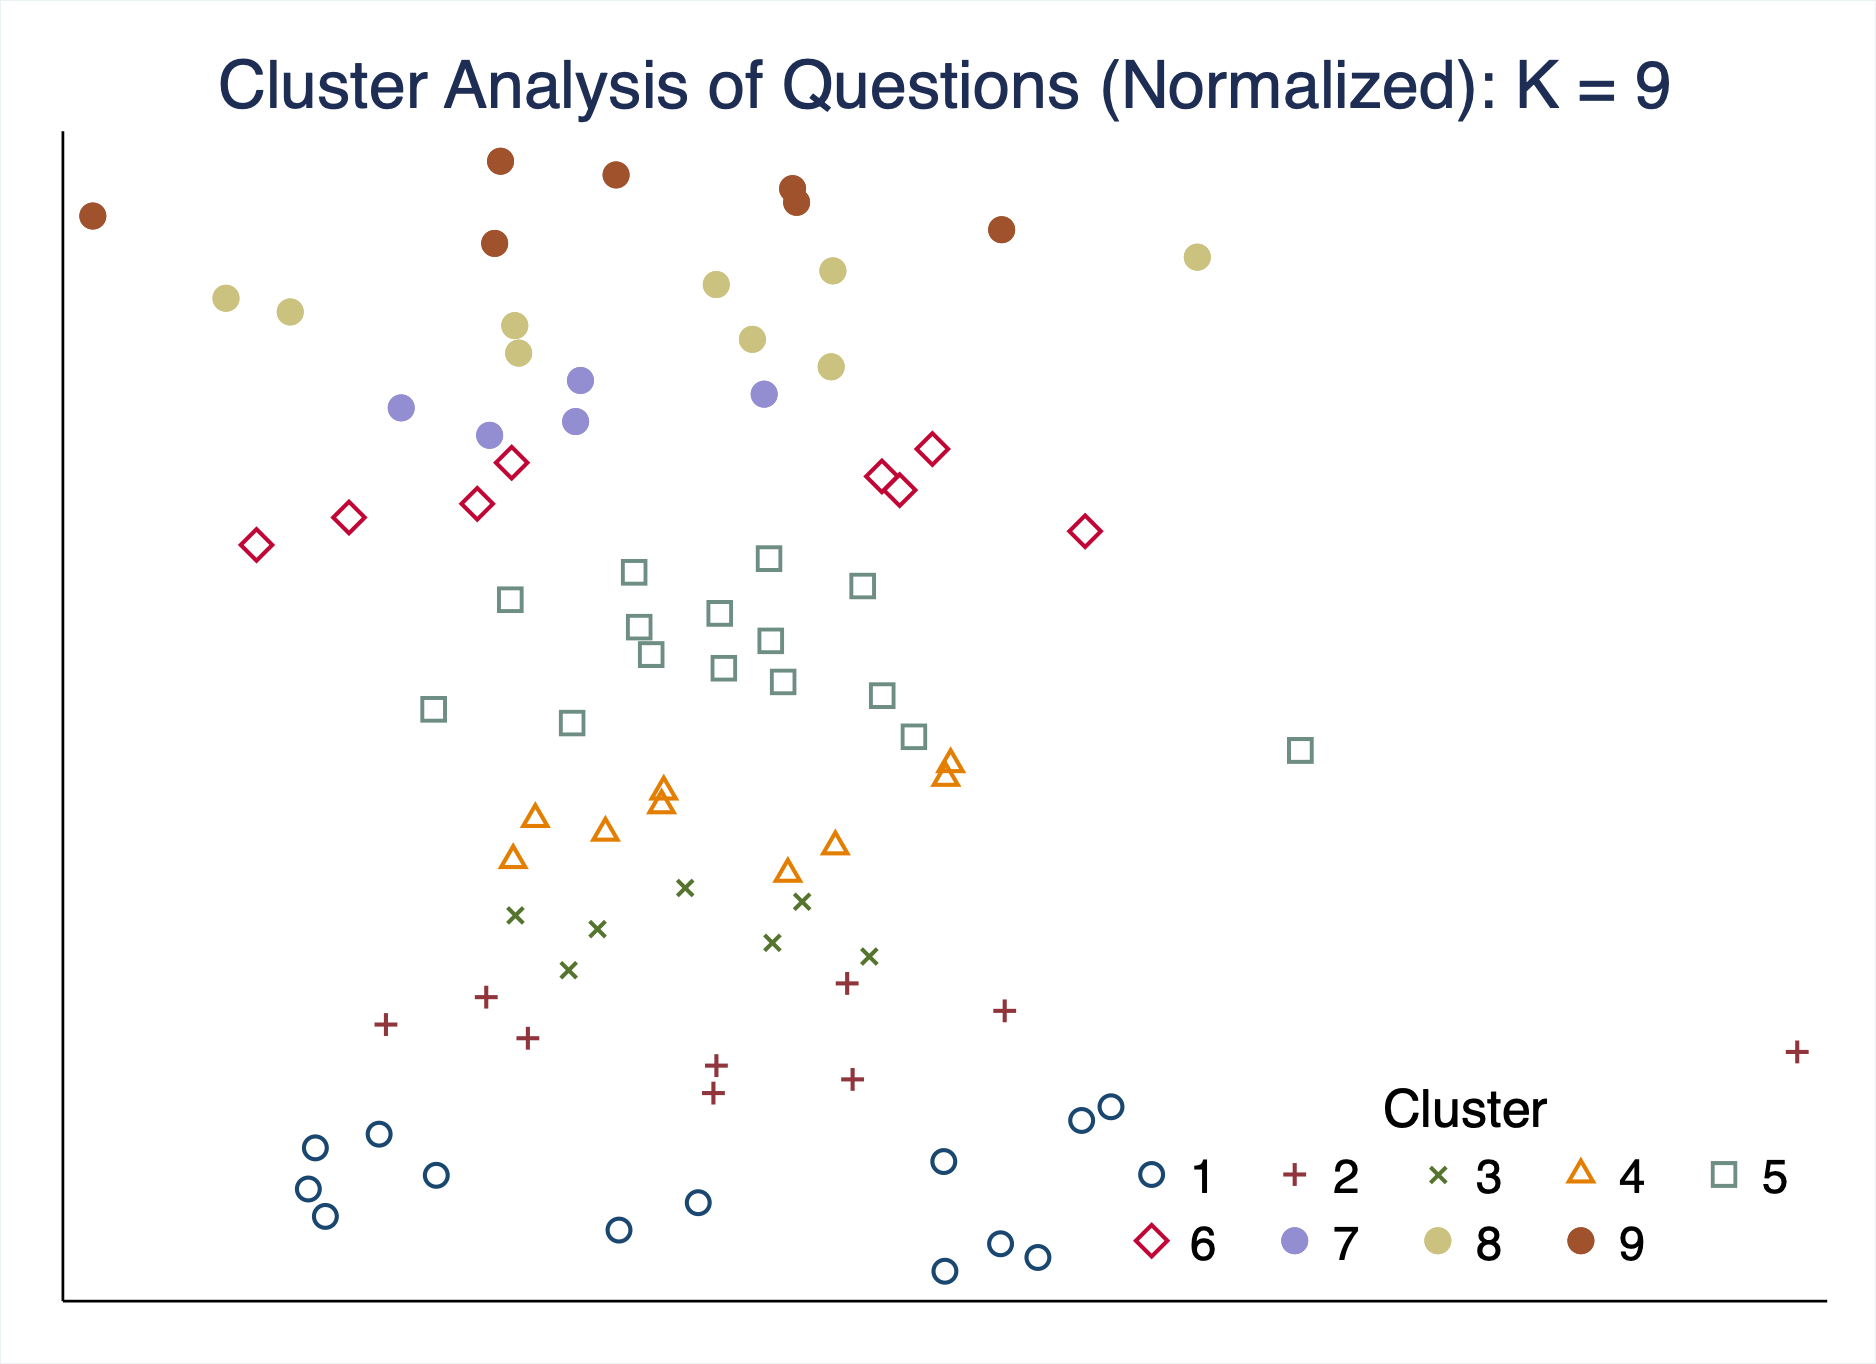
\includegraphics[scale=0.15]{CA_QuestionK9_NOR.png}
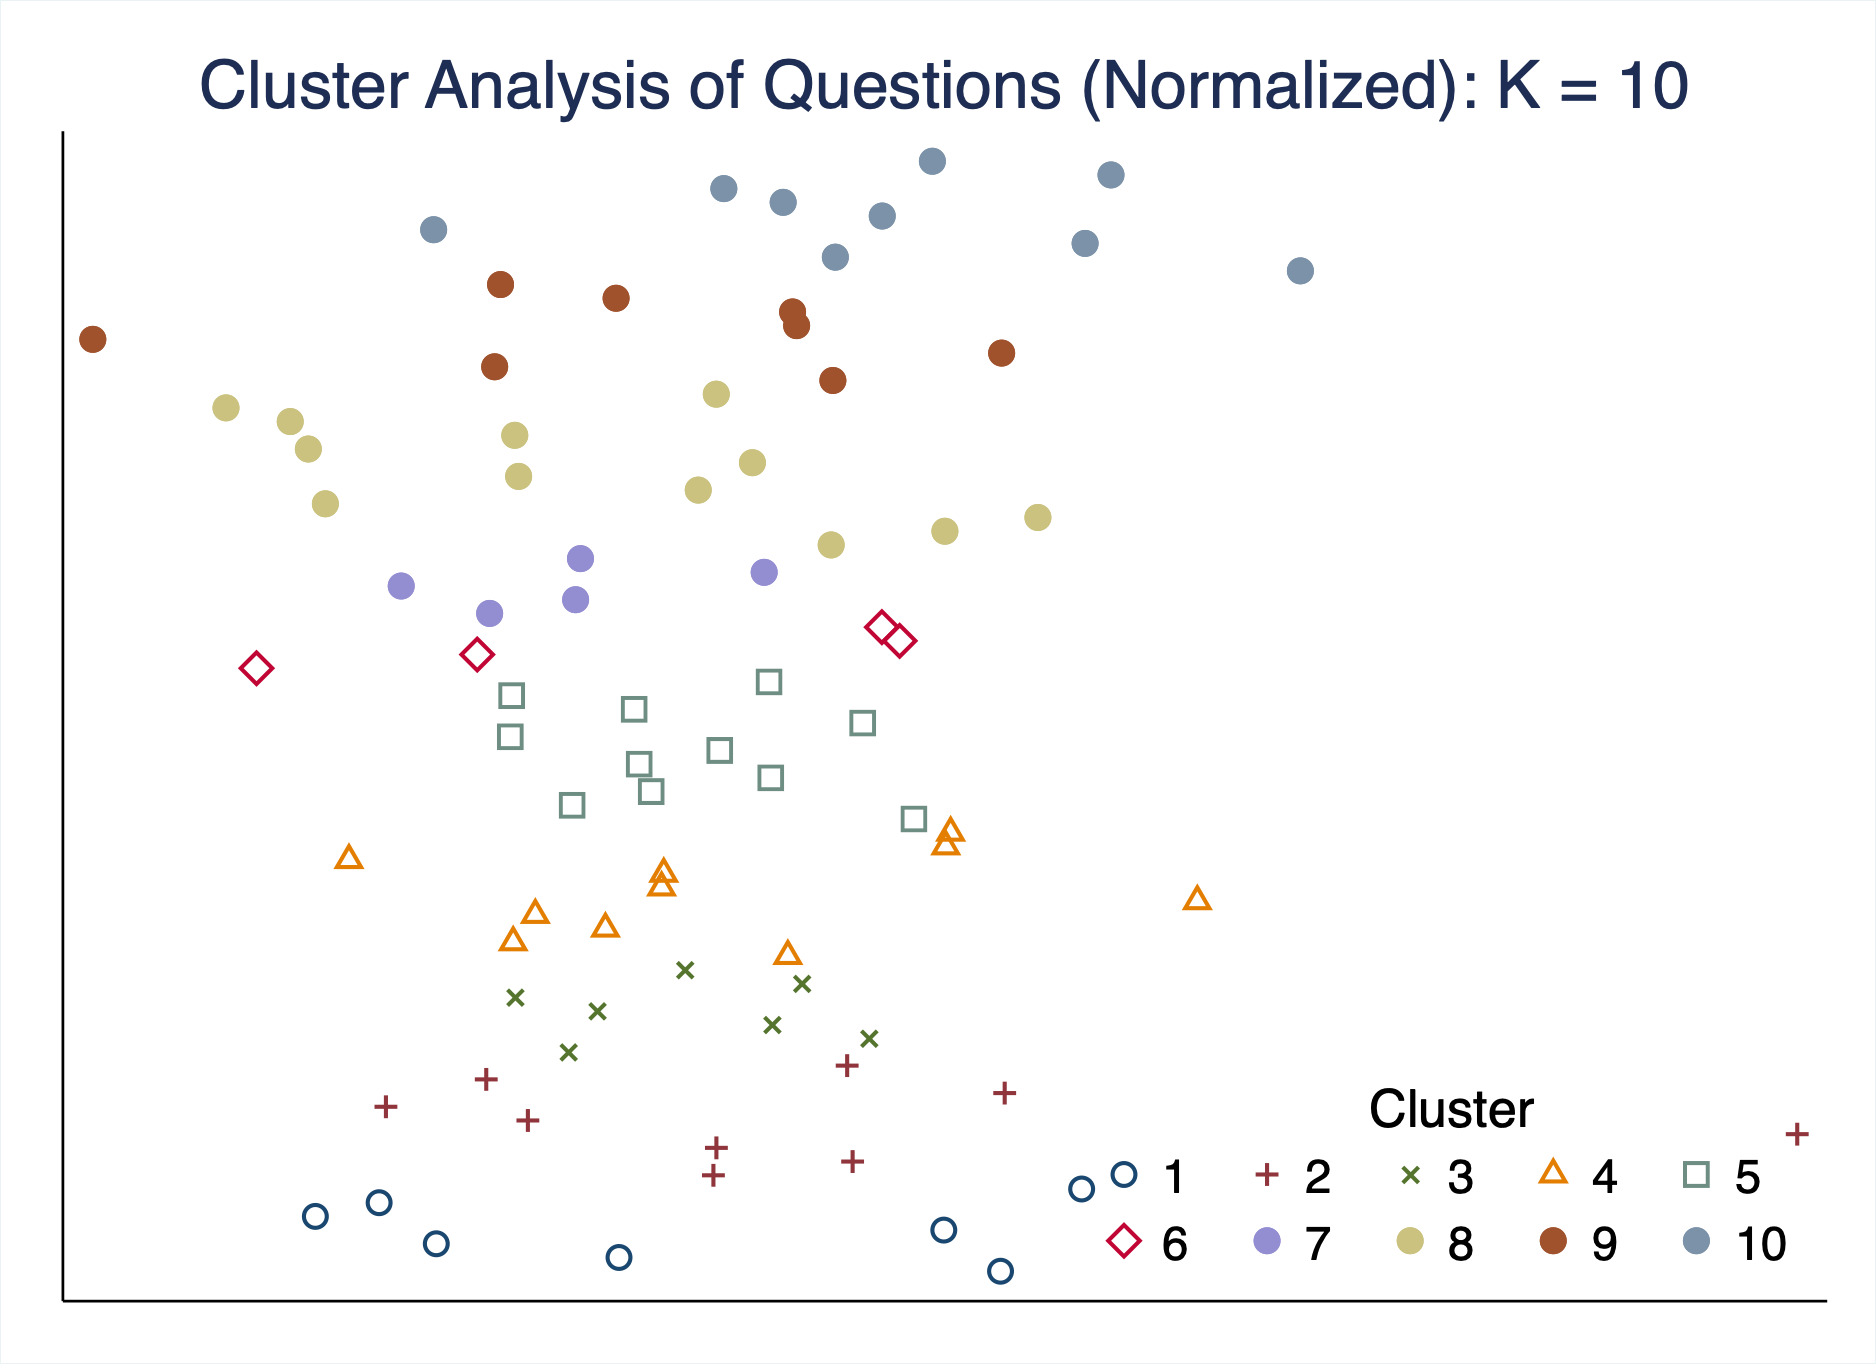
\includegraphics[scale=0.15]{CA_QuestionK10_NOR.png}
\end{center}
By clustering the questions for the normalized data, we can see that the resulting groups seem to have a similar dispersion of means. This is because, the way we normalized the data is that it all centered around the mean zero and standard deviation one. However, the cluster analysis made it possible to define the pattern and do a good job in clustering it similarly to the ones with non-normalized data, which although it is not seem to be shown in the graph, the resulting groups are similar with the ones with non-normalized data. 
\end{figure}  

\begin{figure}  [h!]
\begin{center}
\caption{Cluster analysis of questions with normalized data (K=5)}
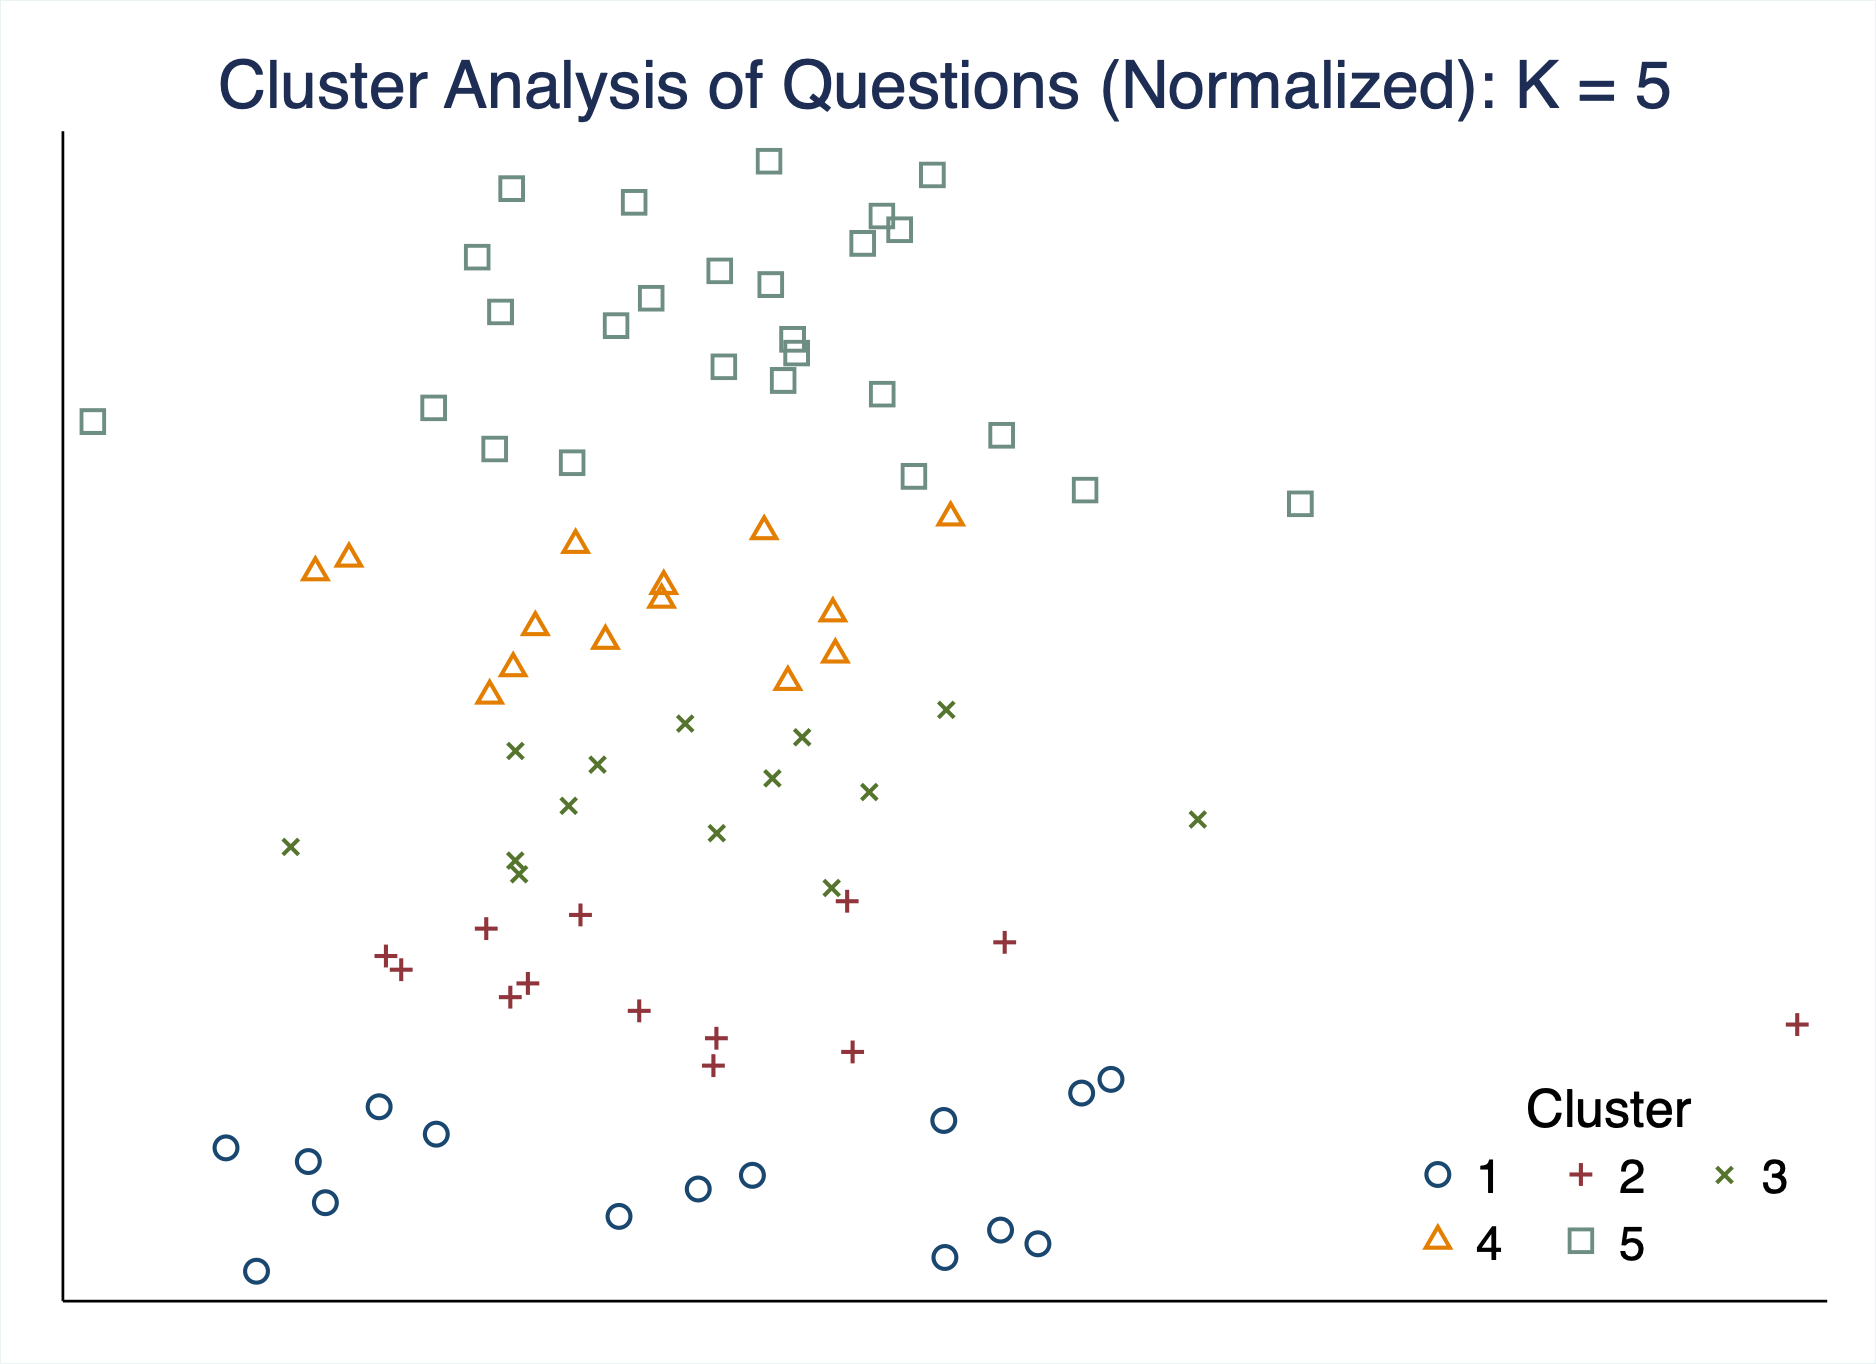
\includegraphics[scale=0.25]{CA_QuestionK5_NOR.png}
\end{center}
\end{figure}  

\begin{figure}  [h!]
\subsubsection{Country clustering}
\begin{center}
\caption{Cluster analysis of country with normalized data}
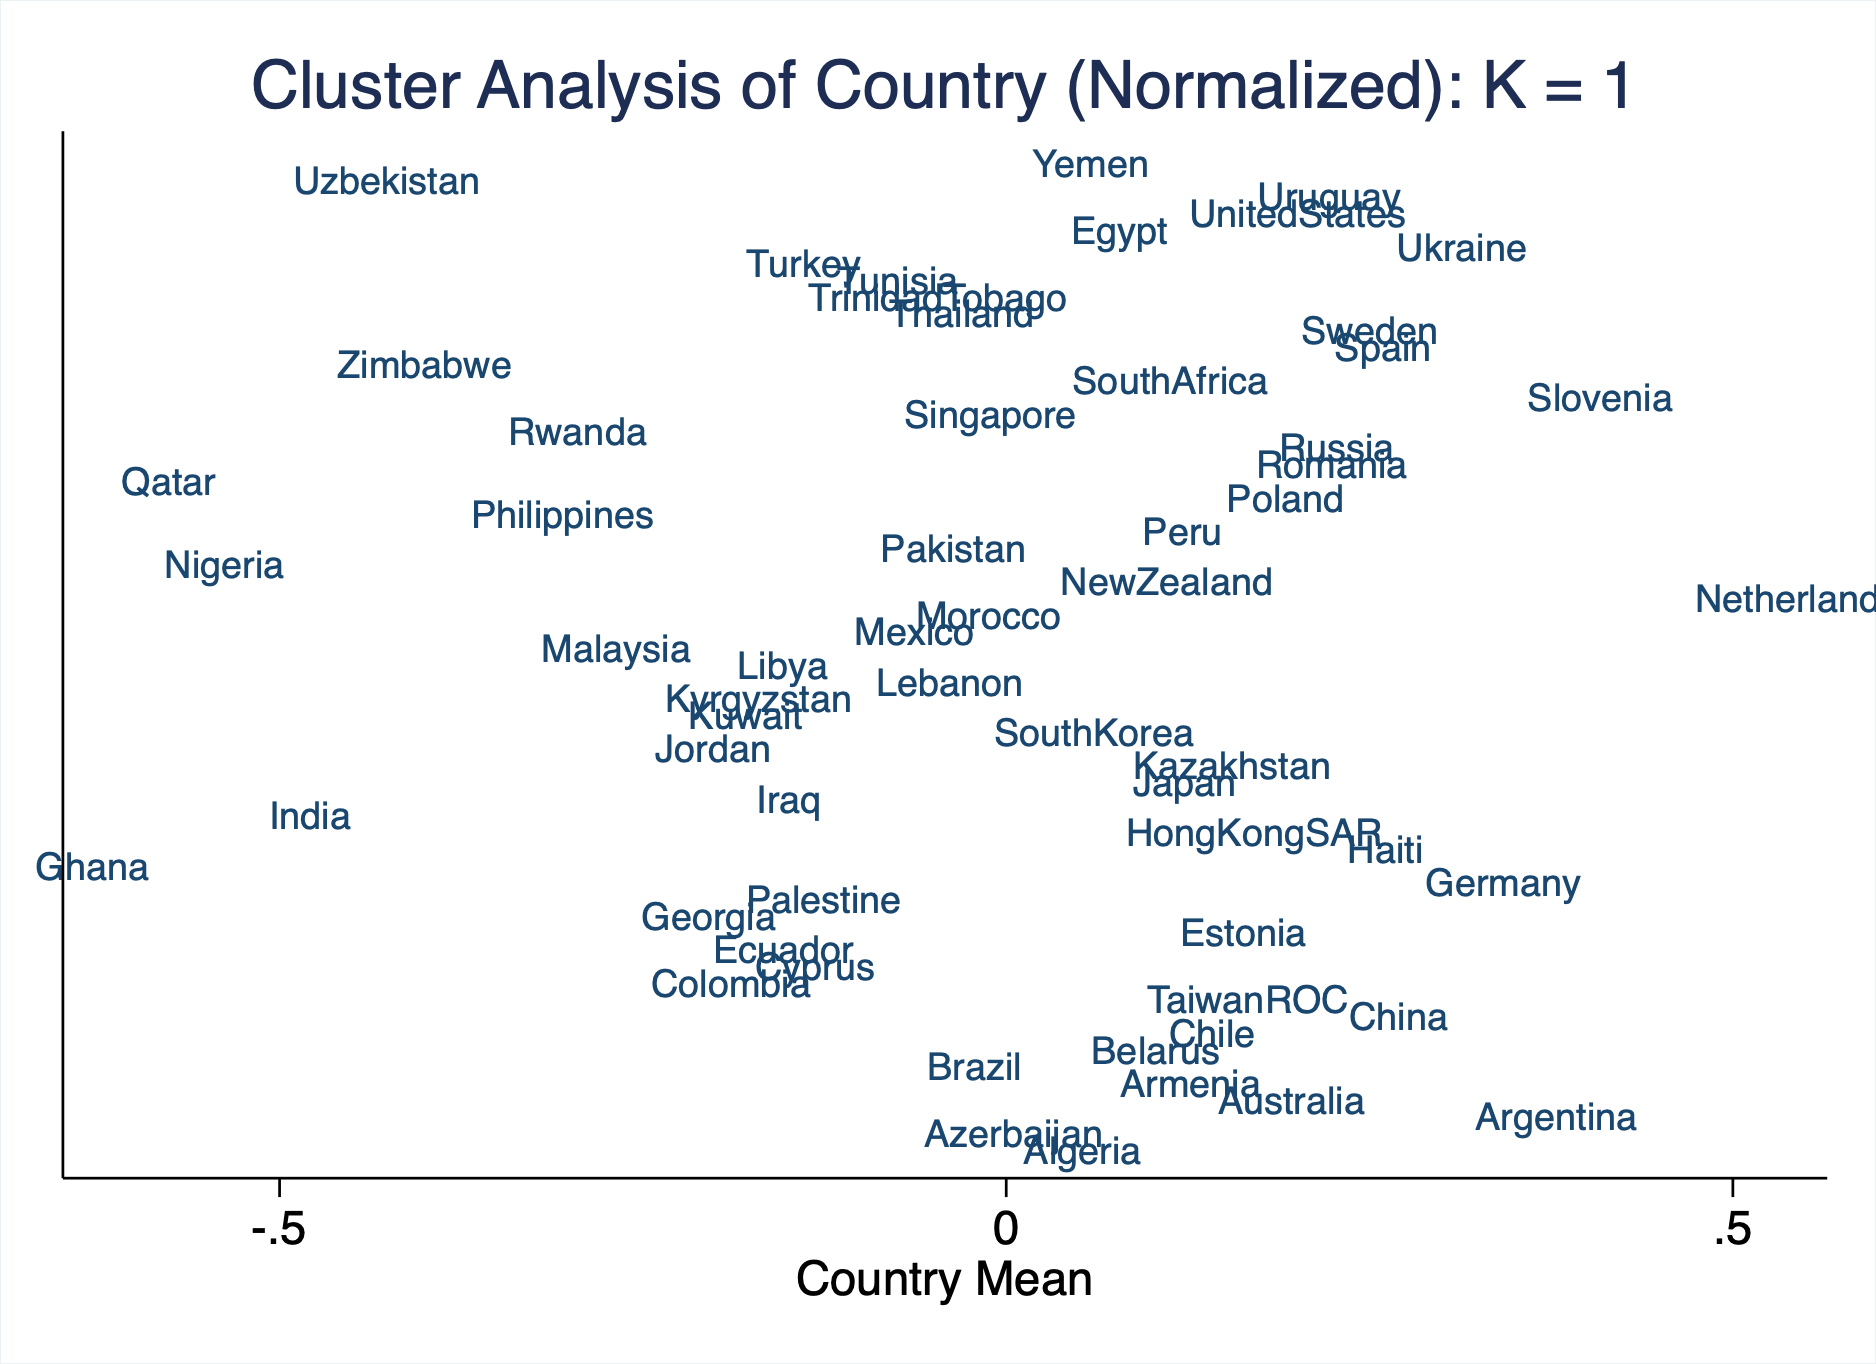
\includegraphics[scale=0.15]{CA_CountryK1_NOR.png}
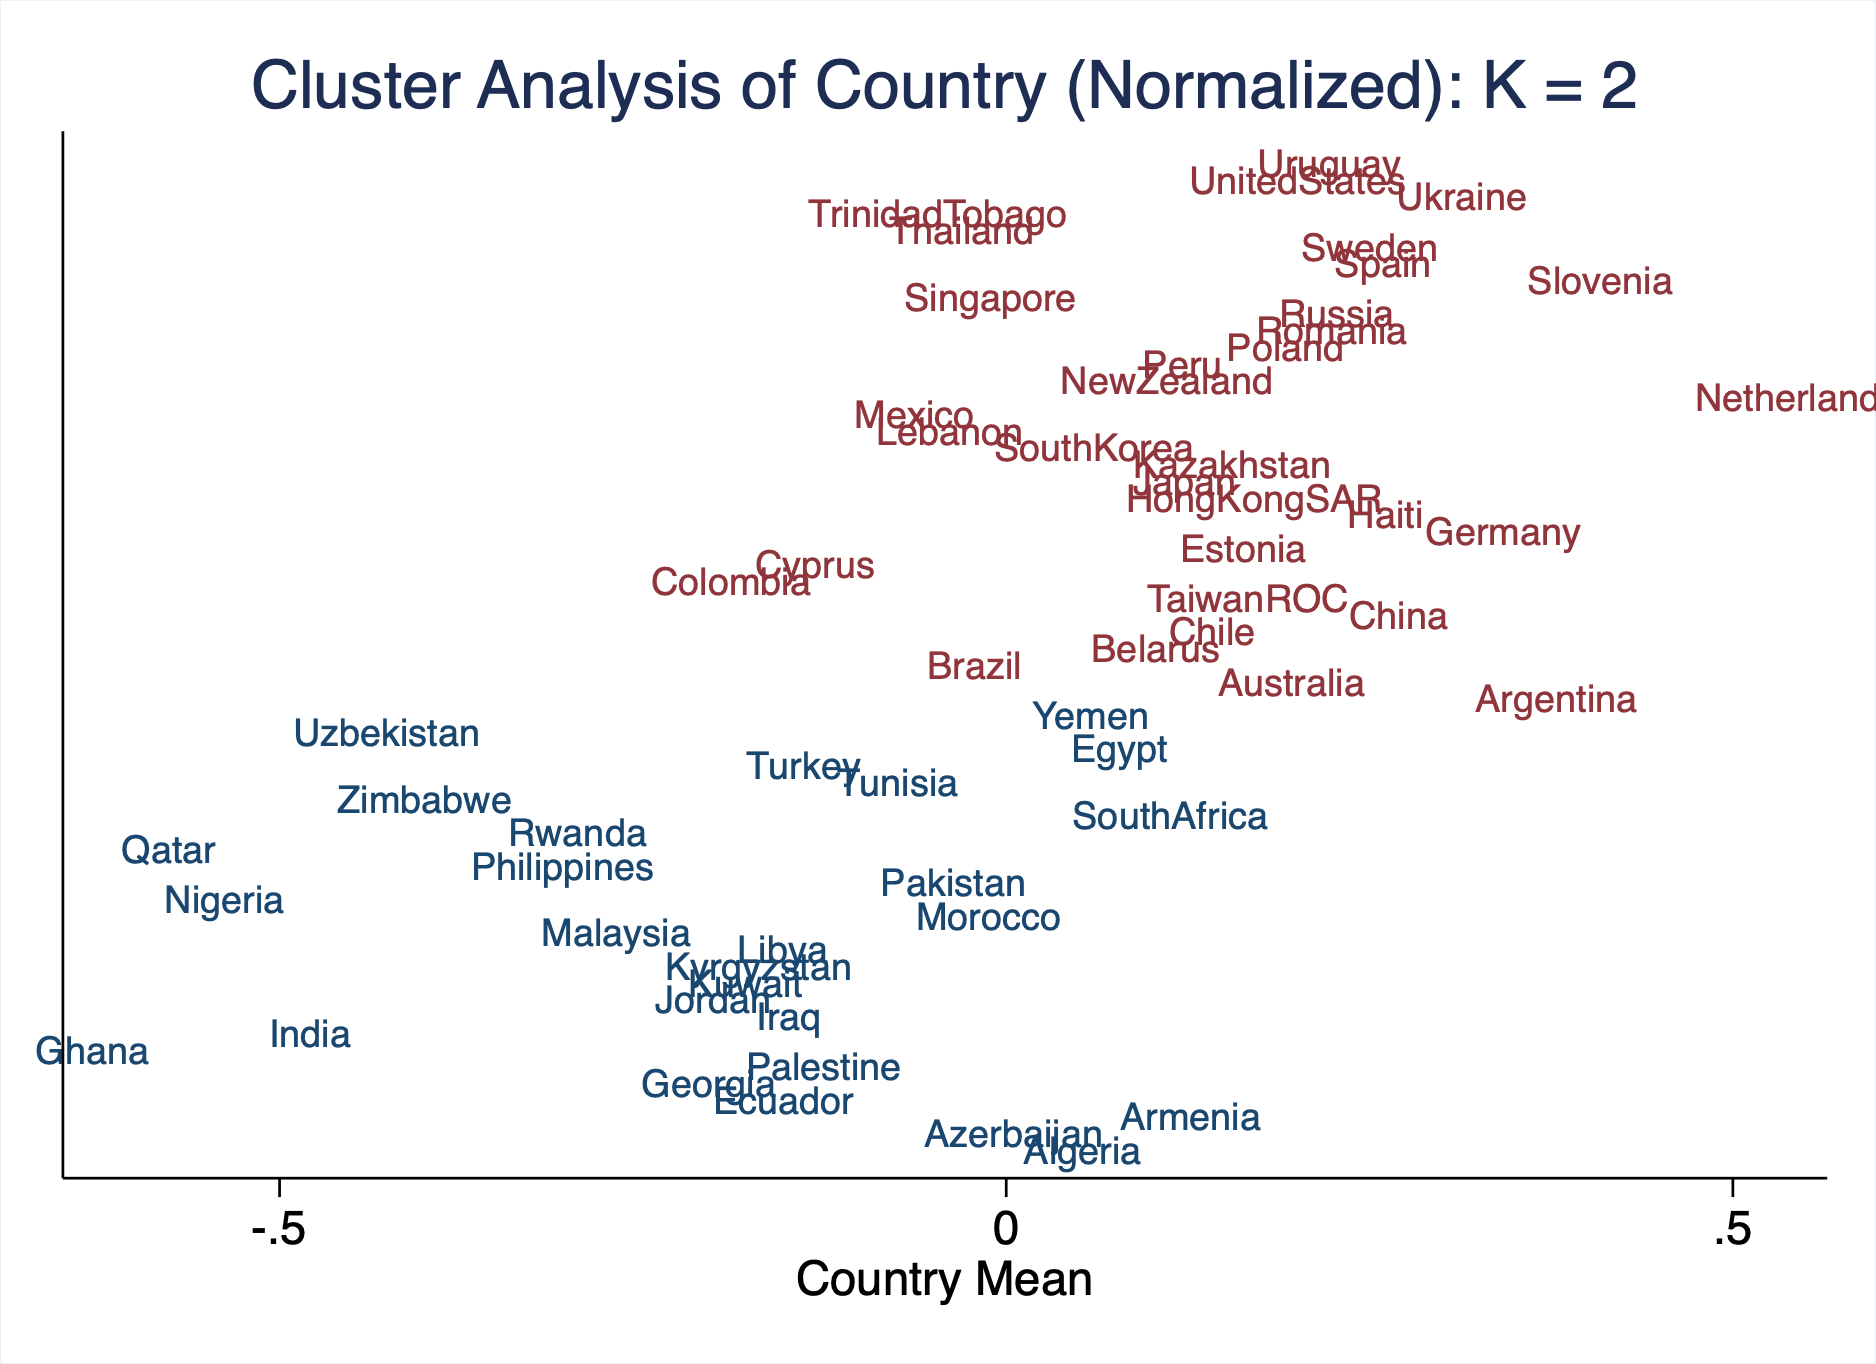
\includegraphics[scale=0.15]{CA_CountryK2_NOR.png}
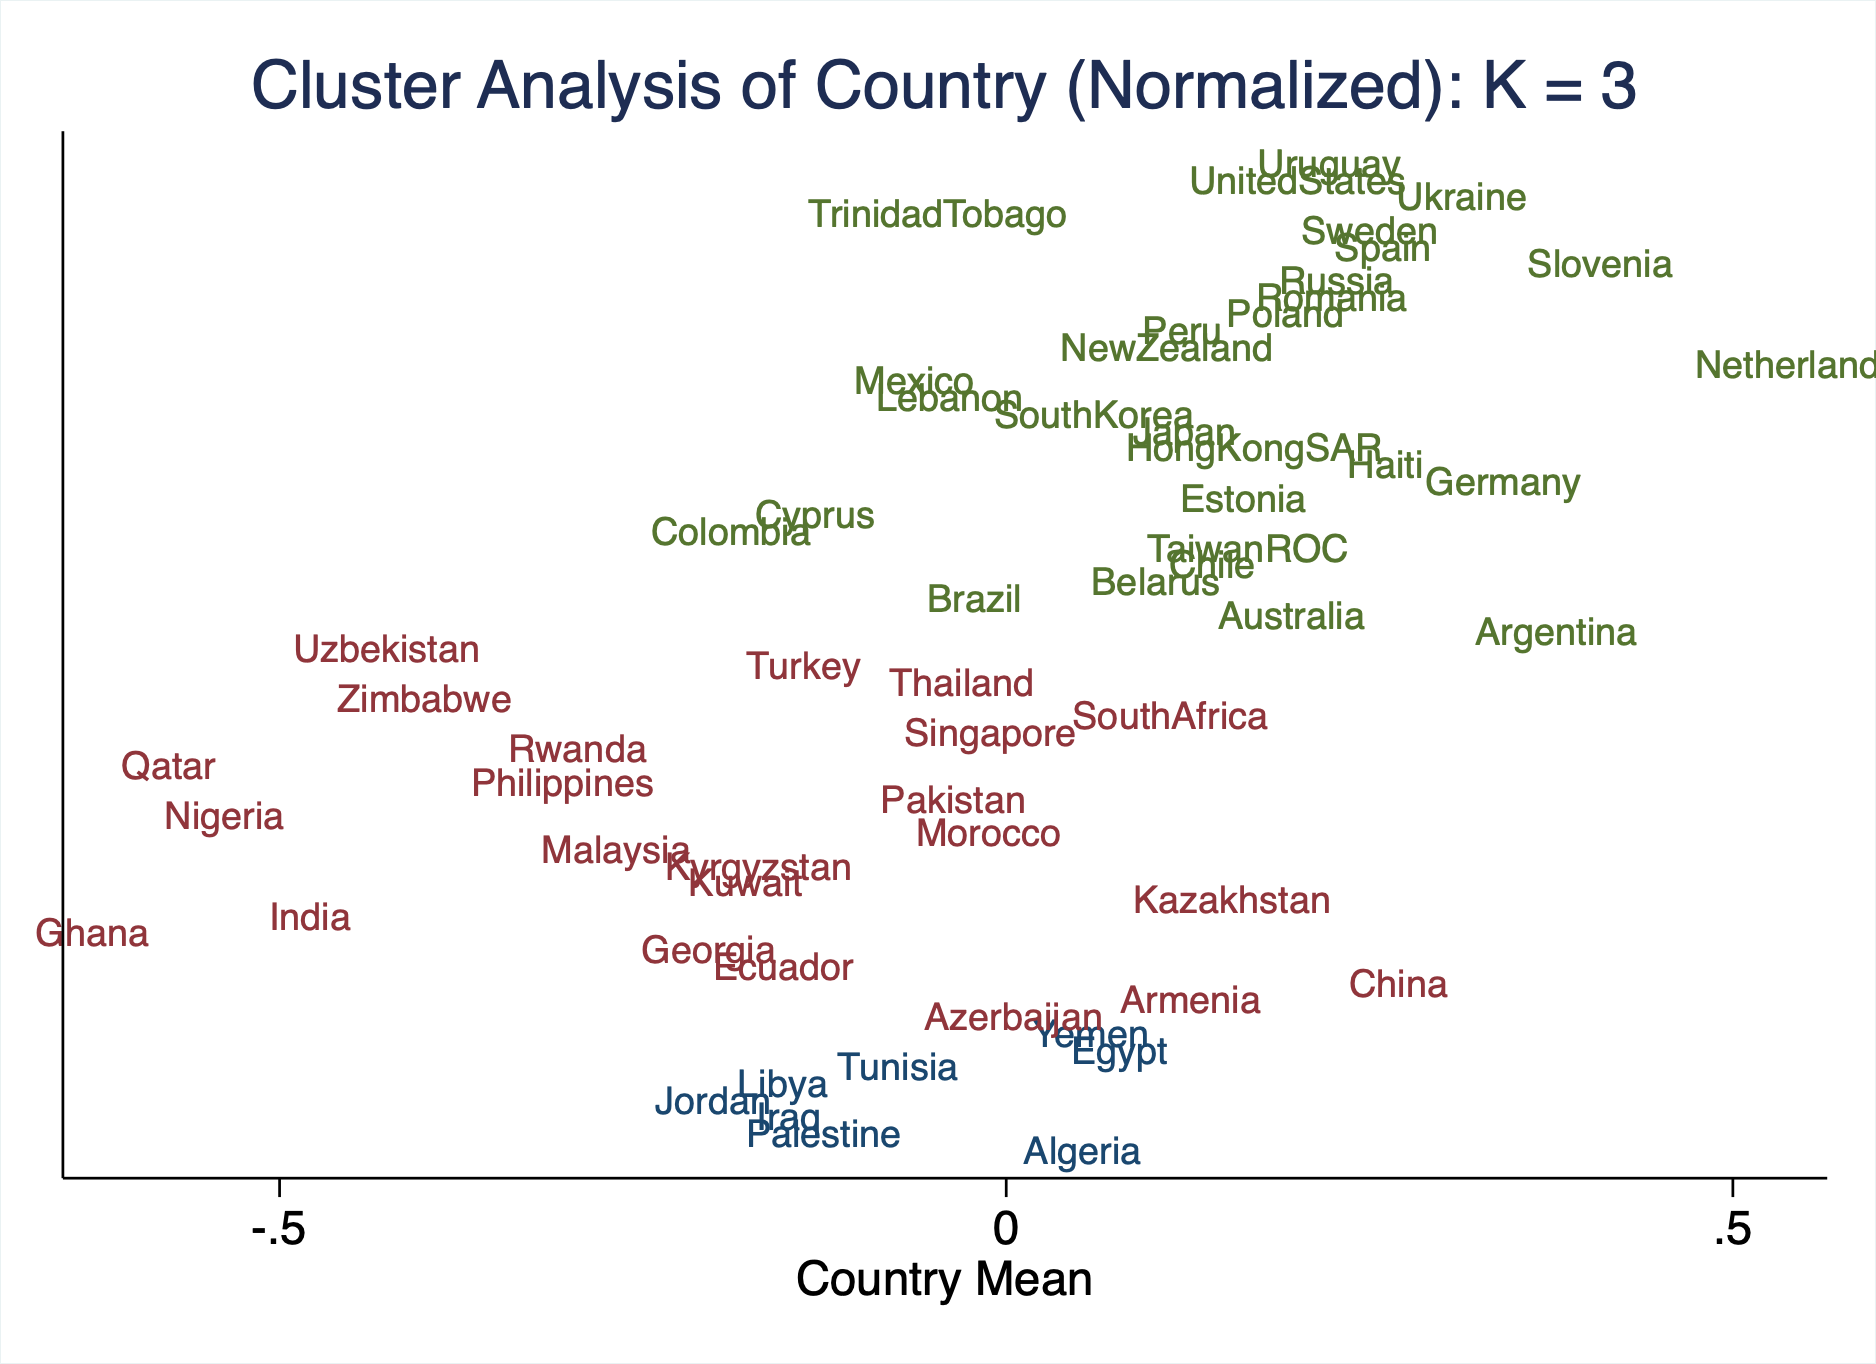
\includegraphics[scale=0.15]{CA_CountryK3_NOR.png}
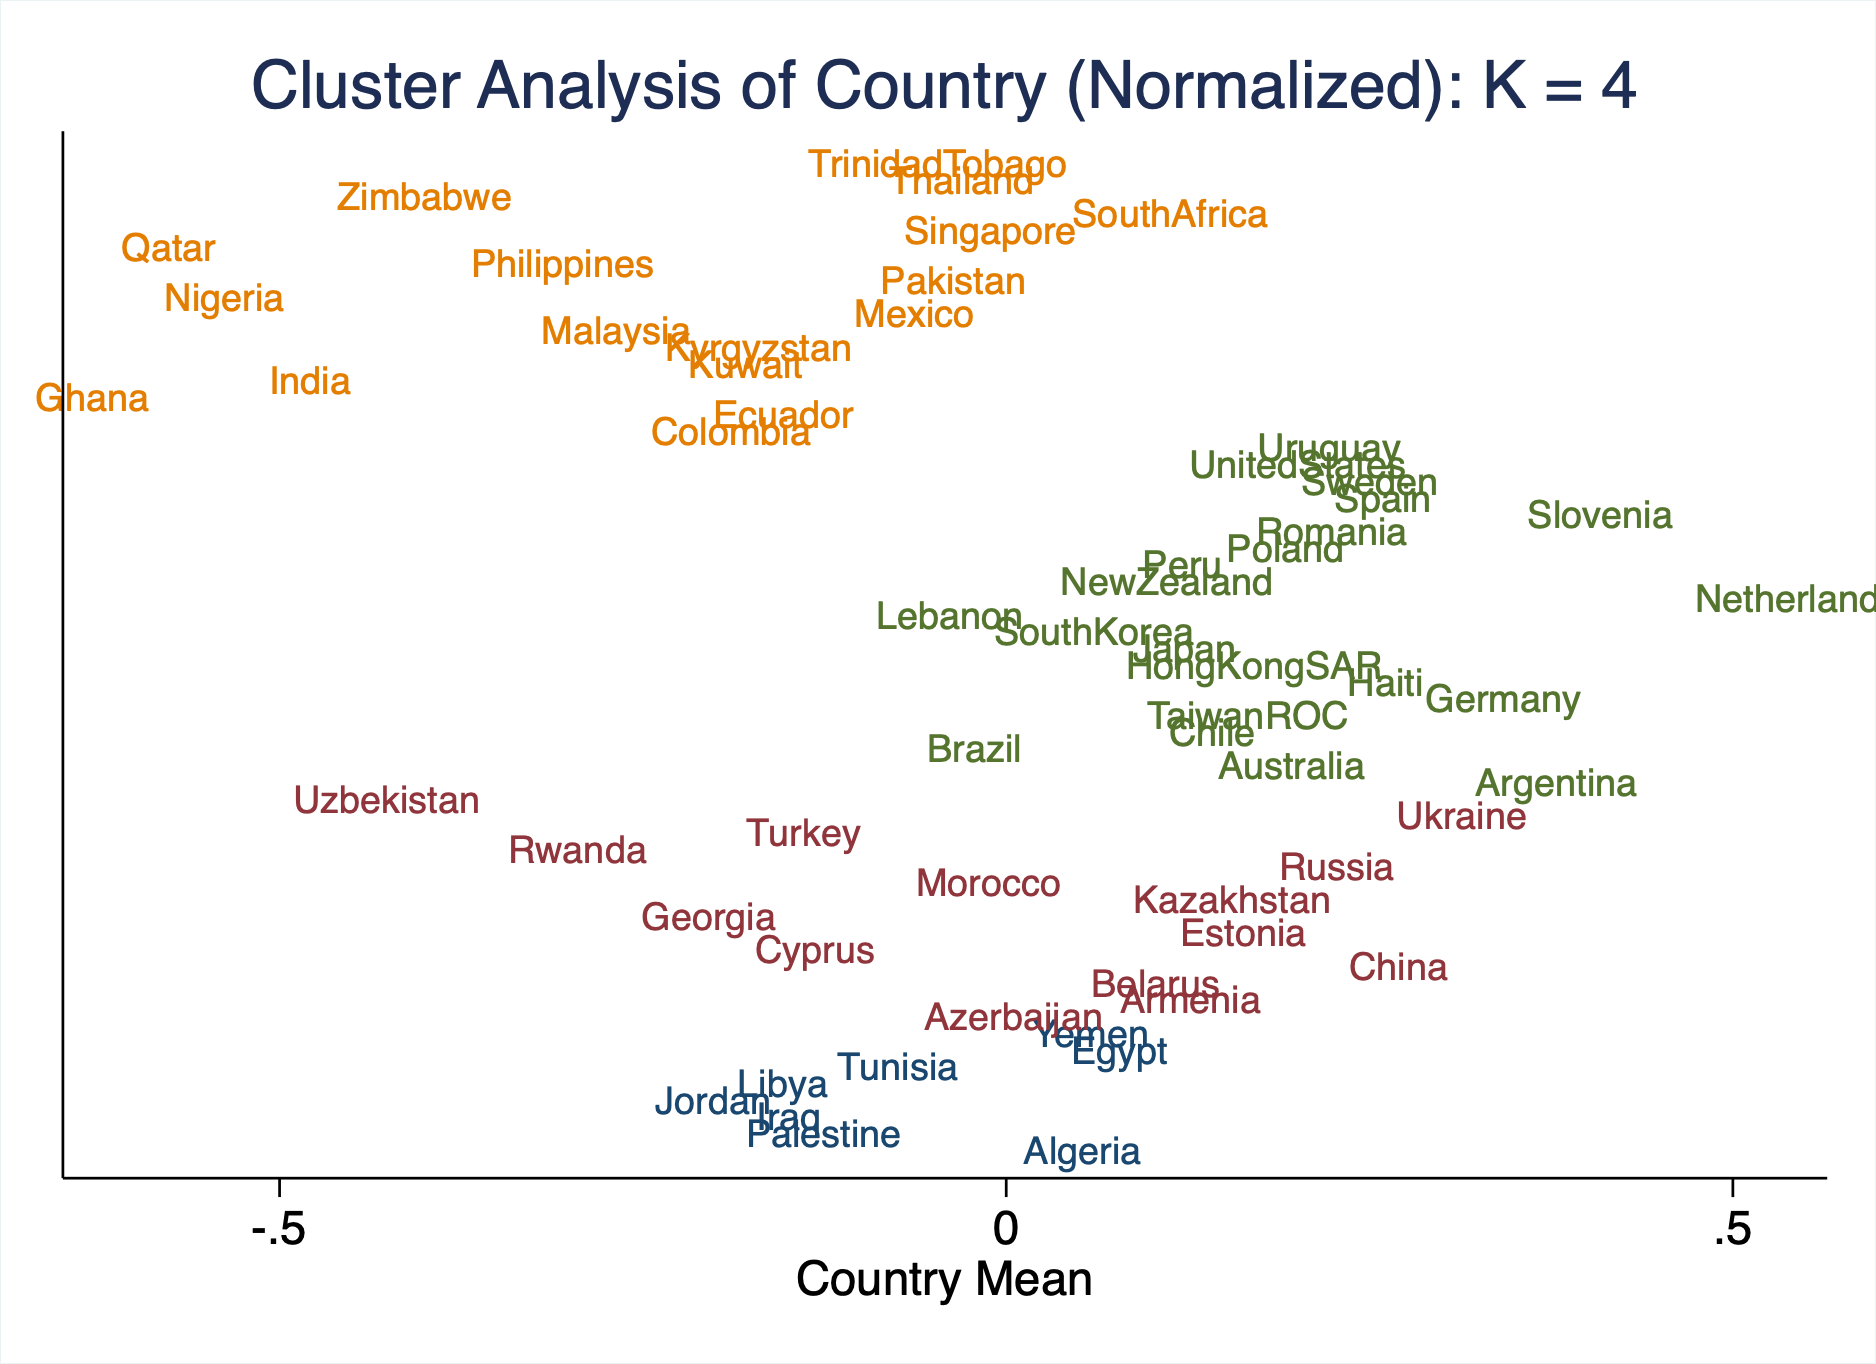
\includegraphics[scale=0.15]{CA_CountryK4_NOR.png}
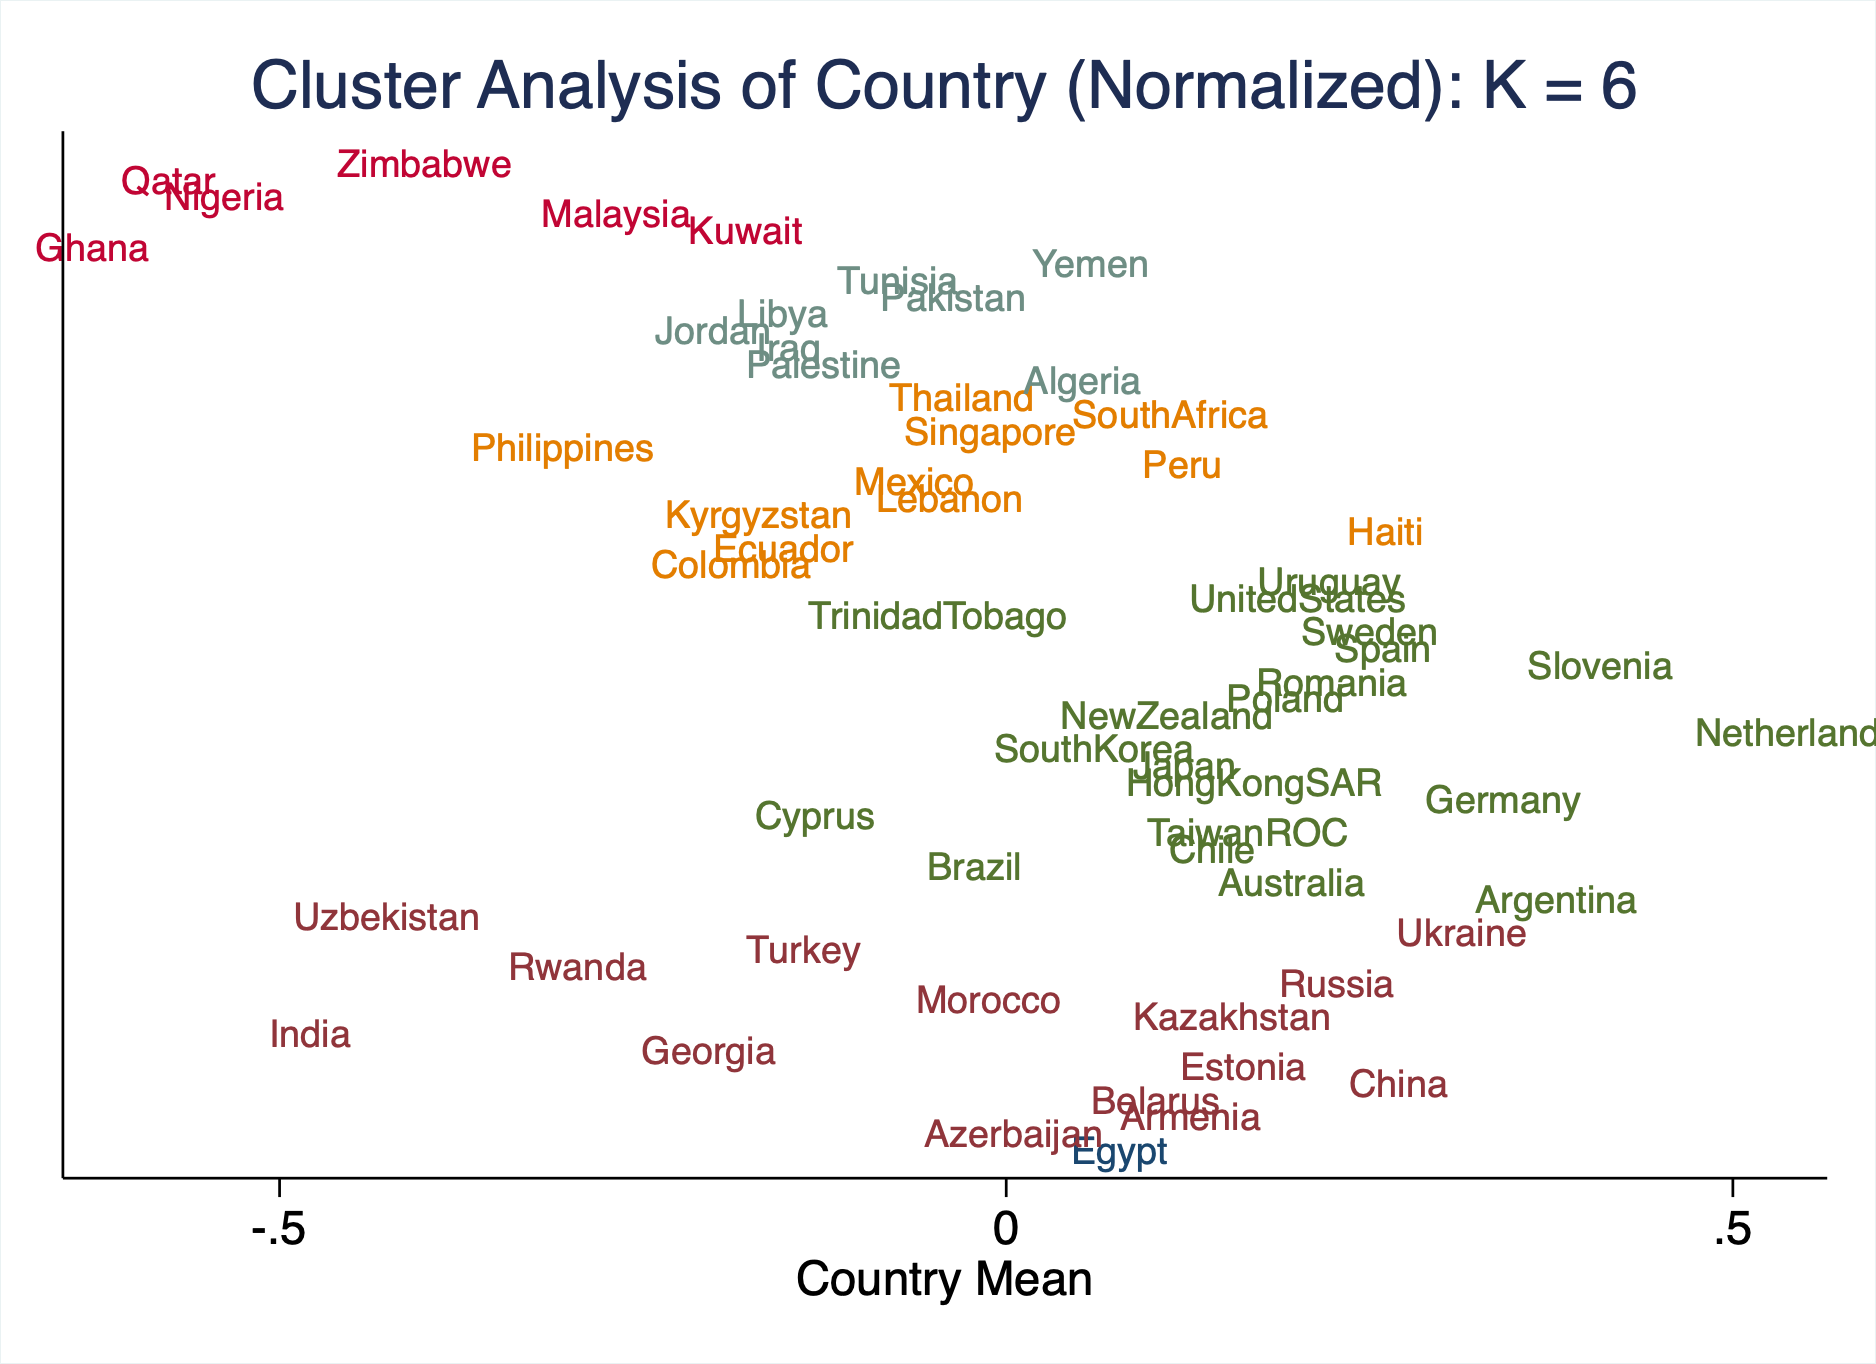
\includegraphics[scale=0.15]{CA_CountryK6_NOR.png}
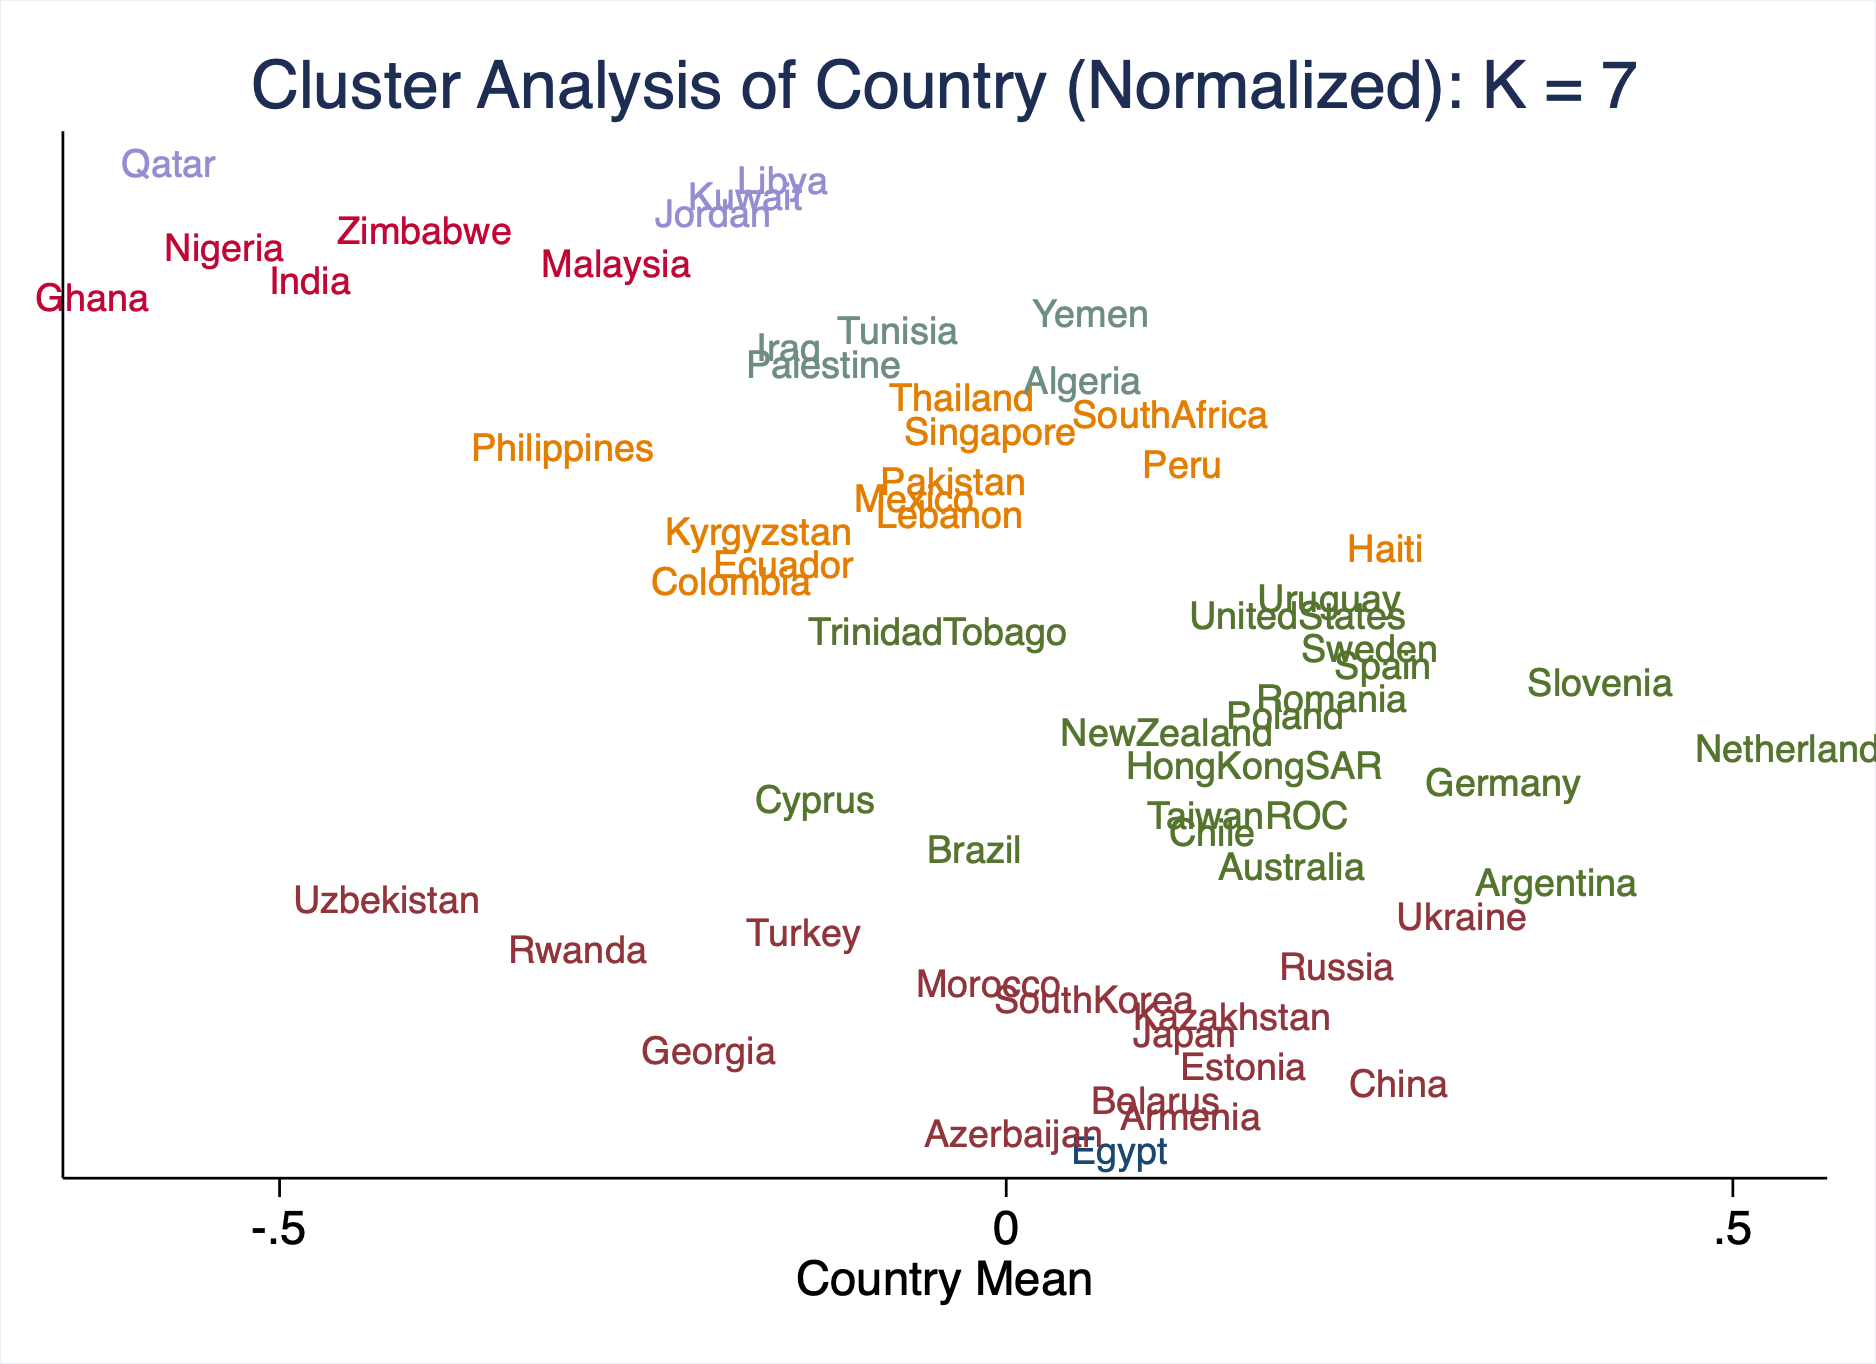
\includegraphics[scale=0.15]{CA_CountryK7_NOR.png}
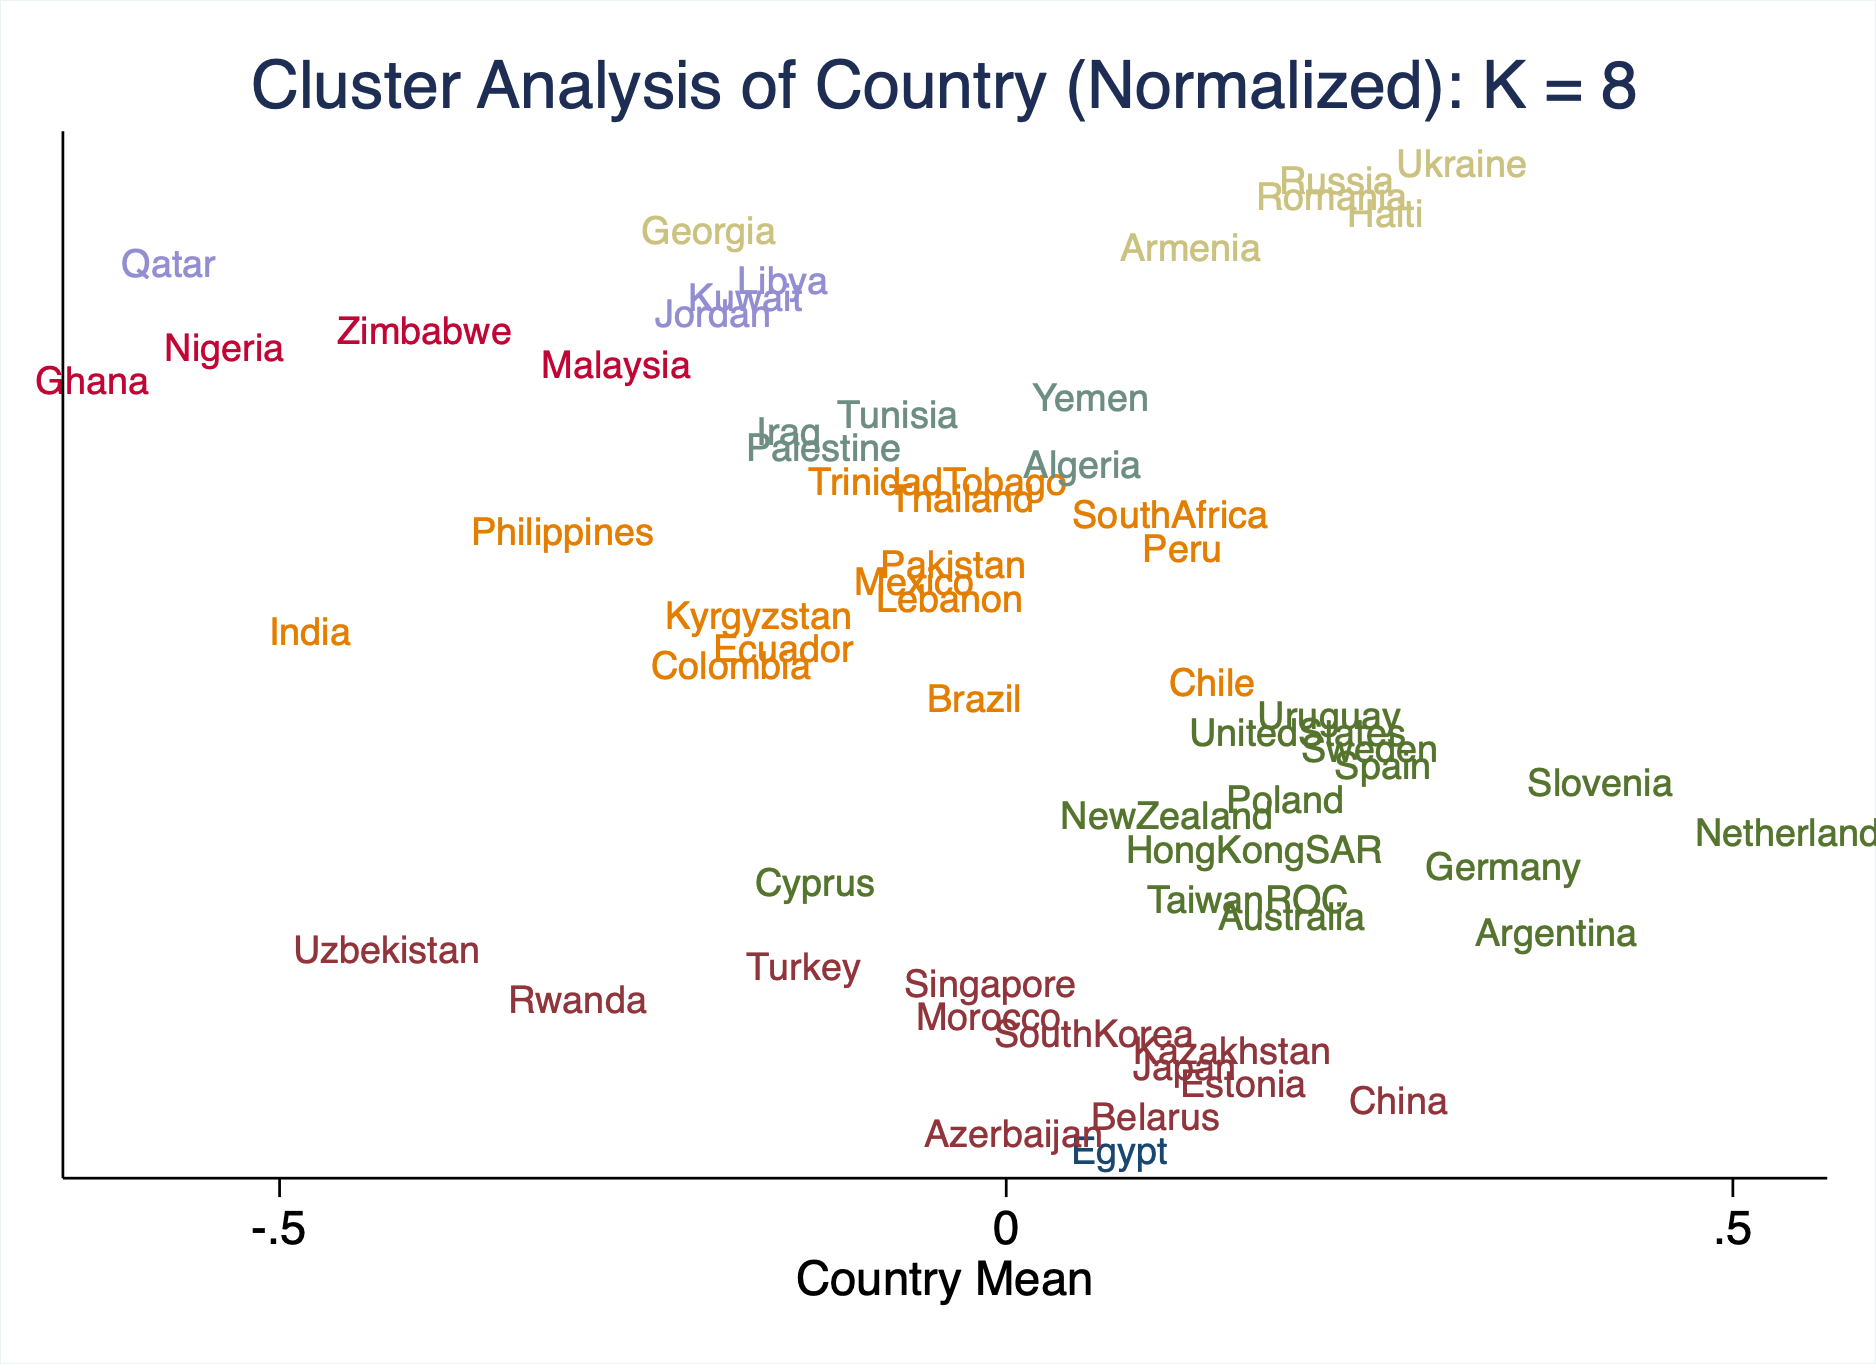
\includegraphics[scale=0.15]{CA_CountryK8_NOR.png}
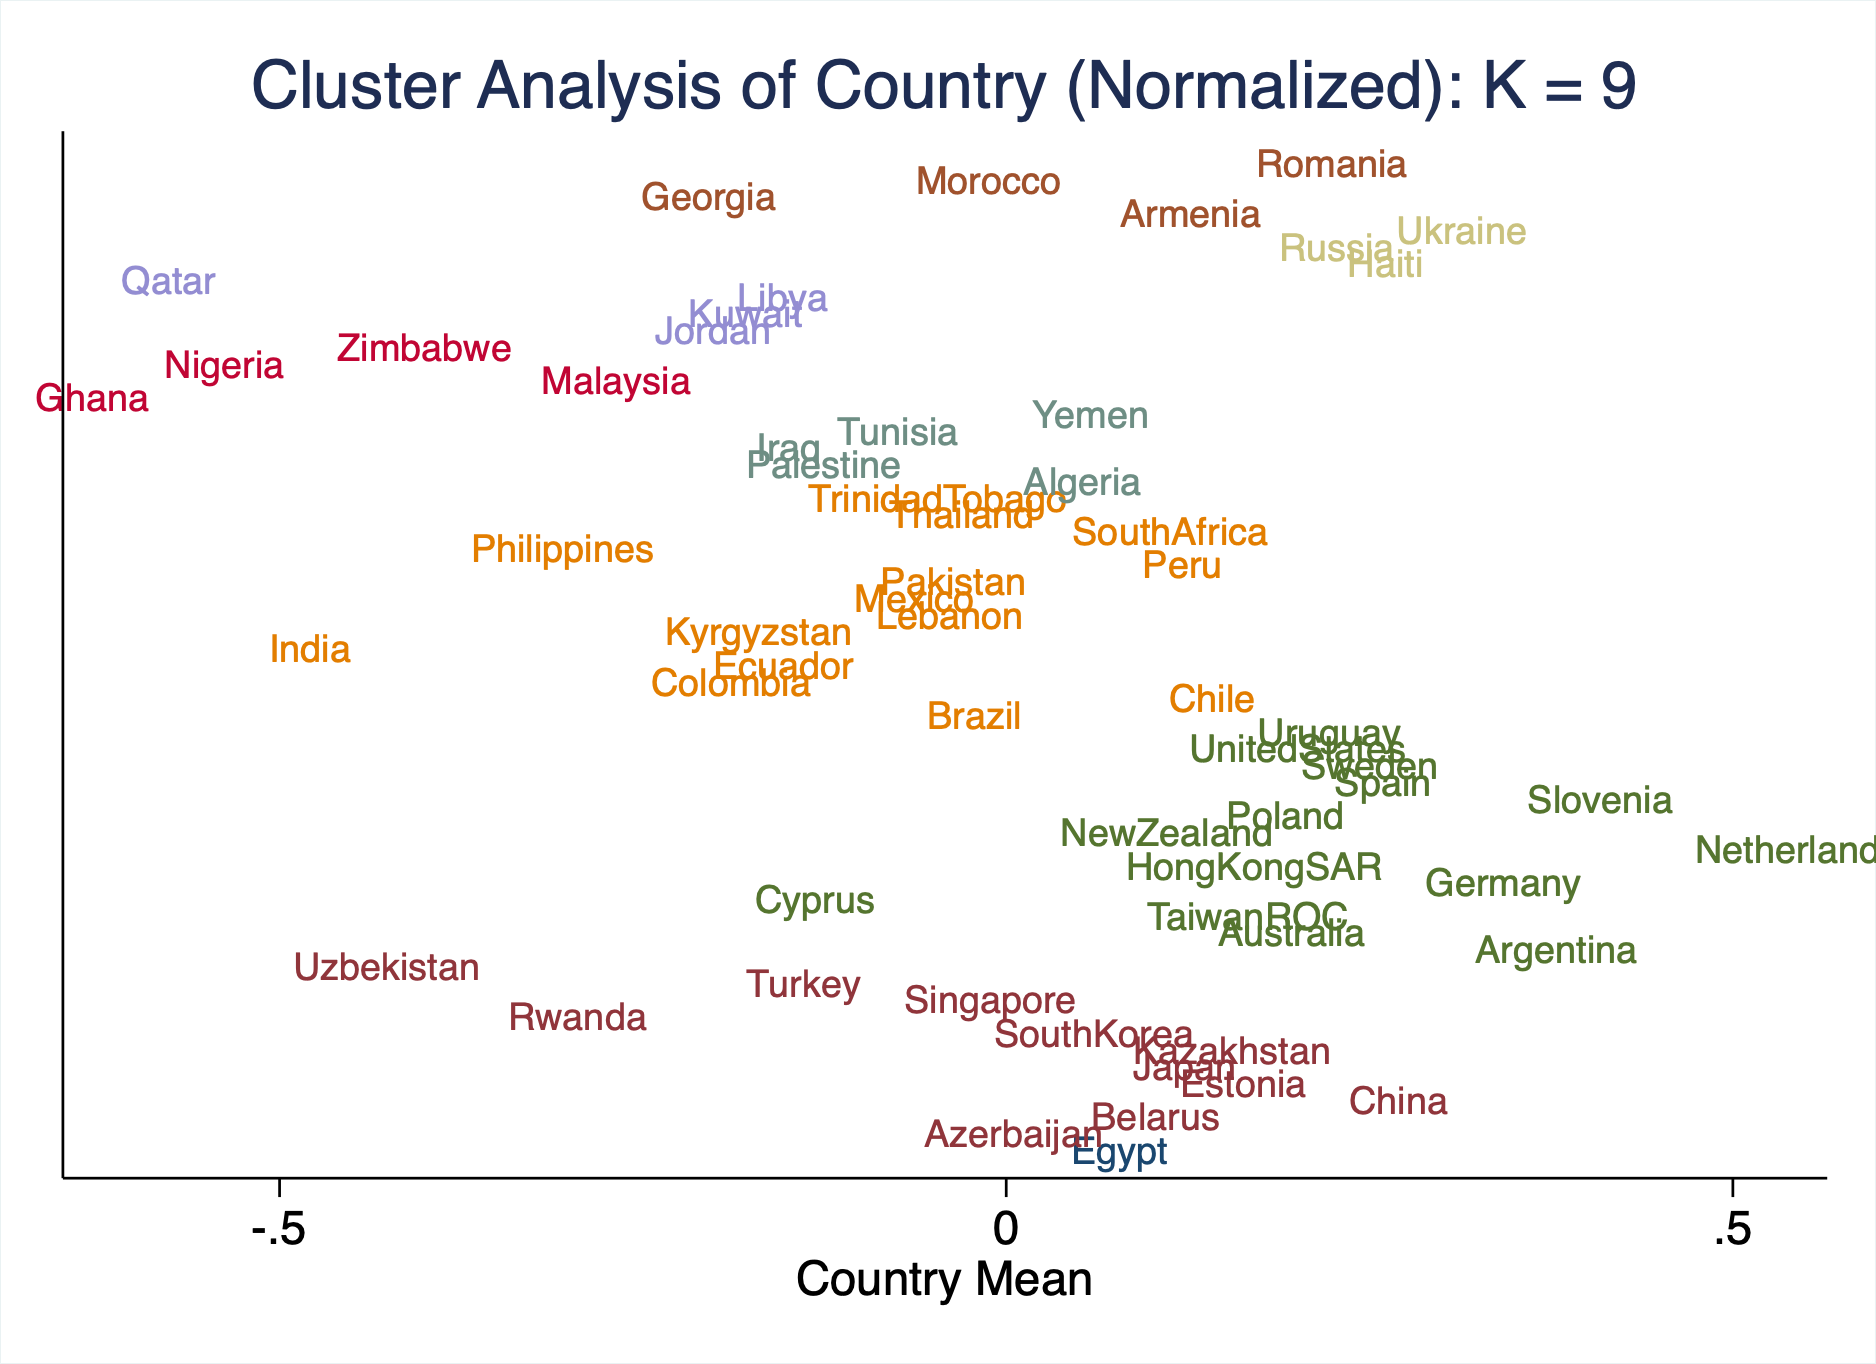
\includegraphics[scale=0.15]{CA_CountryK9_NOR.png}
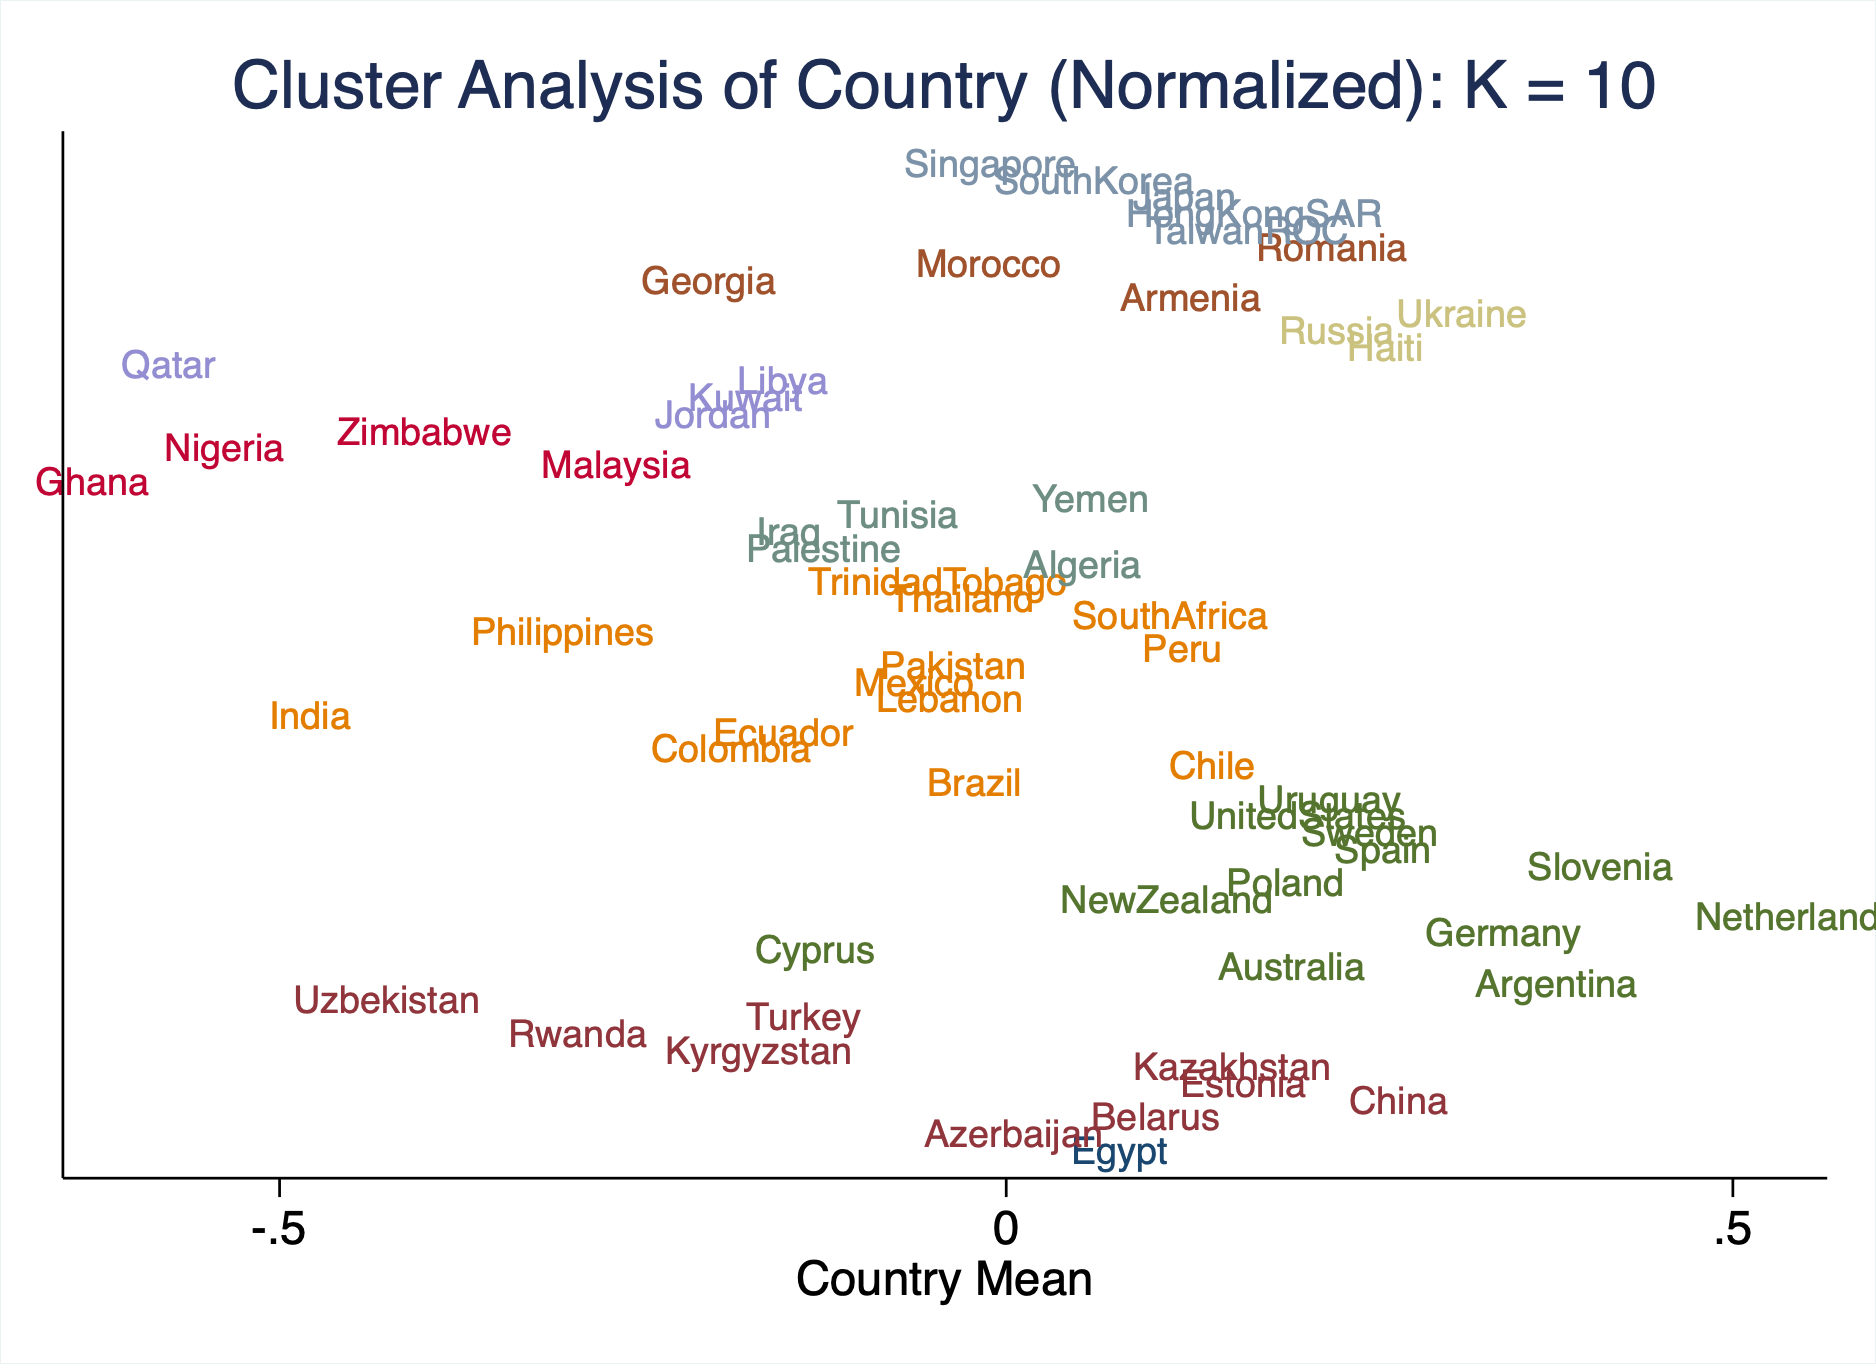
\includegraphics[scale=0.15]{CA_CountryK10_NOR.png}
\end{center}
We observe a similar pattern of clustering with the non-normalized data. This, in essence, makes sense due to the normalization that was done at the question level. Hence, unlike the normalized question clustering, we see that each cluster is grouped in a rather concentrated means. 
\end{figure}  

\begin{figure}  [h!]
\begin{center}
\caption{Cluster analysis of country with normalized data (K=5)}
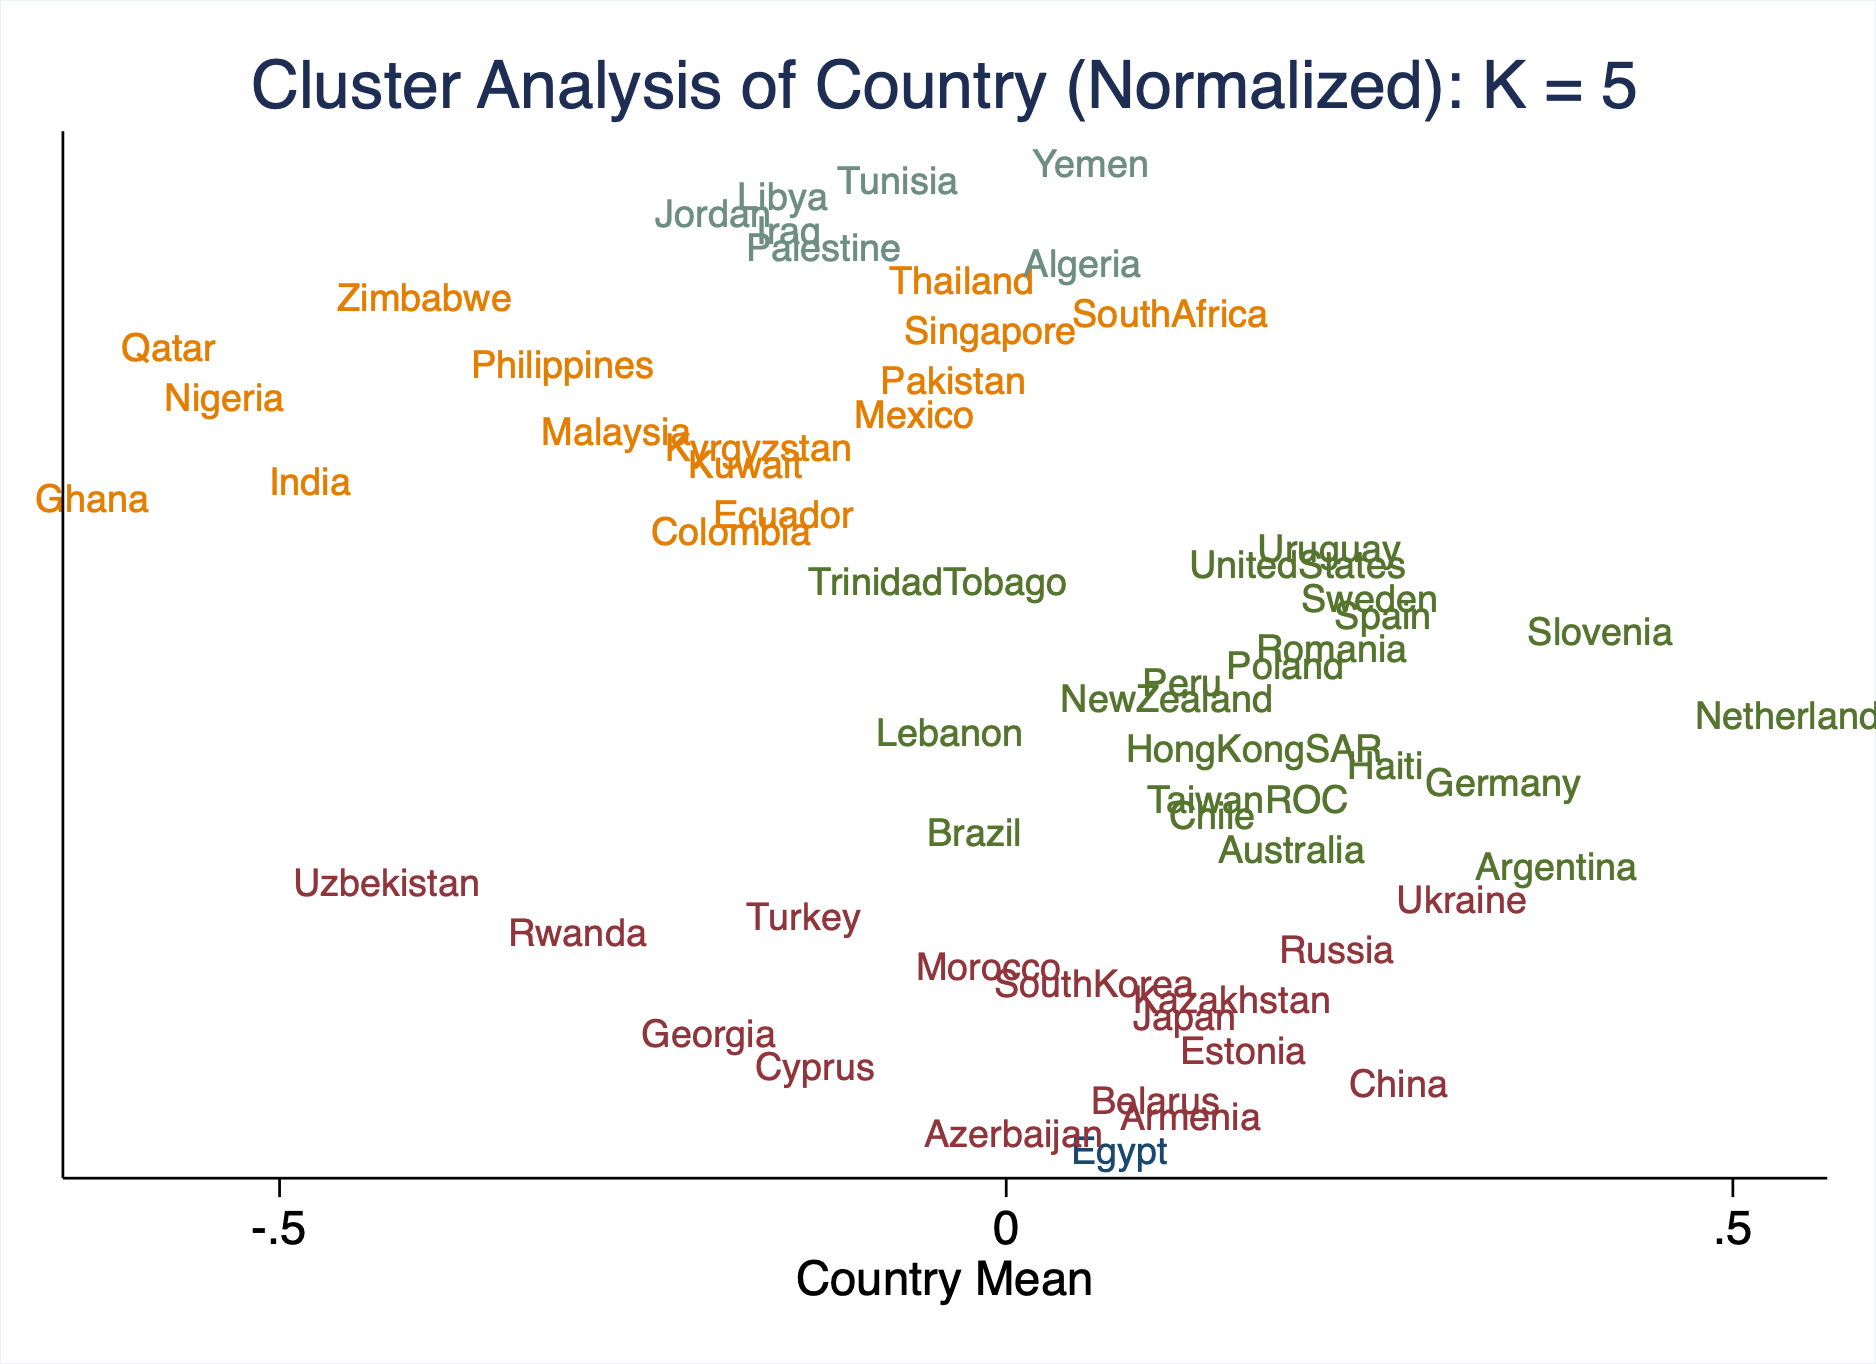
\includegraphics[scale=0.25]{CA_CountryK5_NOR.png}
\end{center}
\end{figure}  



\pagebreak
\begin{figure}  [h!]
\section{Principal Component Analysis}
For the PCA, the figure depicted below is more of a biplot rather than a culture map. But this is interesting given how the interpretation could be different from the culture map depicted in the lecture note. The first component put more weight in the traditional values whereas the second component put more weight in the democracy and freedom. Table 2 and 3 presents how each questions are weighted in each component. I used the cluster analysis to group the countries, rather than area.
\\
\subsection{Non-normalized data}
\begin{center}
\caption{PCA culture map with non-normalized data}
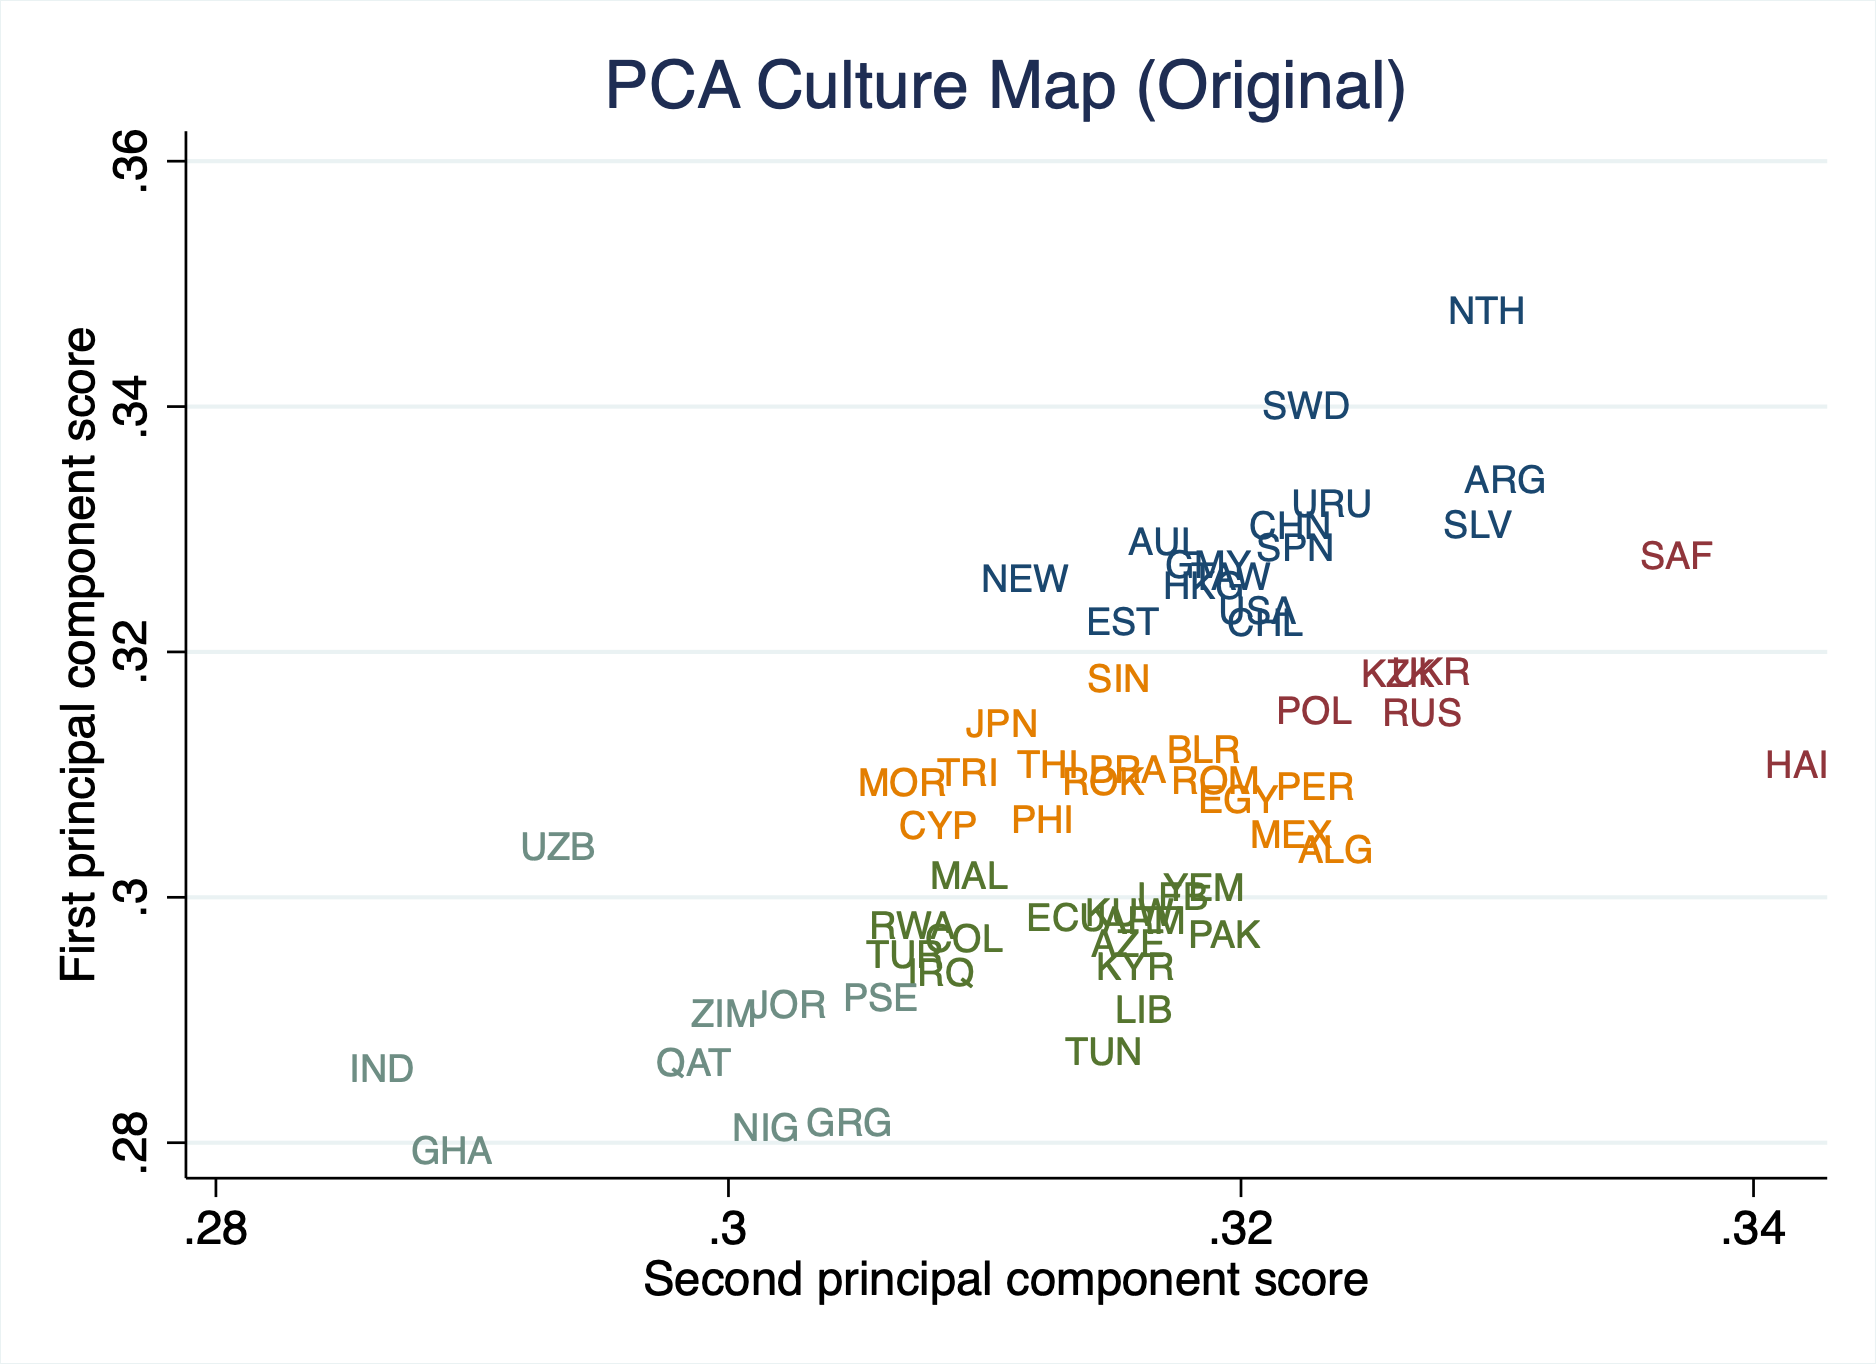
\includegraphics[scale=0.25]{PCA_CultureMap_ORI.png}
\end{center}
Seeing Figure 9, the result seem to show that countries with high democracy and freedom also upholds a higher traditional values. Which is quite contrasting to the result shown in the lecture note. 
\end{figure} 

\begin{table}[tbp]
\centering
\caption{PCA factor loading for two components (non-normalized data)}
\begin{adjustbox}{width=0.7\textwidth}
\small


\begin{tabularx}{\linewidth}{@{}lCC@{}}

\toprule
{Question Code}&{Factor Loading PC1}&{Factor Loading PC2} \tabularnewline
\midrule \addlinespace[\belowrulesep]
V49&.2078106&.0658256 \tabularnewline
V9&.2017511&.0373875 \tabularnewline
V153&.2016577&.0314327 \tabularnewline
V132&.199843&.0211471 \tabularnewline
V205&.1874759&.079644 \tabularnewline
V53&.1823724&.0495819 \tabularnewline
V139&.1805832&.0364045 \tabularnewline
V75&.1788874&.0352874 \tabularnewline
V182&.1774179&.0284611 \tabularnewline
V51&.1764657&.0915946 \tabularnewline
V52&.1737652&.0117149 \tabularnewline
V71&.1696302&.004705 \tabularnewline
V183&.1689363&.0242158 \tabularnewline
V184&.1667707&.0295192 \tabularnewline
V77&.1618756&.0688607 \tabularnewline
V138&.1602611&.1039313 \tabularnewline
V8&.1559734&.0437046 \tabularnewline
V108&.1557414&.1039401 \tabularnewline
V79&.1544669&.0982276 \tabularnewline
V181&.1501807&.0503627 \tabularnewline
V72&.1487002&.0325913 \tabularnewline
V208&.1458341&.090243 \tabularnewline
V190&.1418065&.1053625 \tabularnewline
V76&.1339771&.0371005 \tabularnewline
V188&.1331382&.1314552 \tabularnewline
V209&.1327176&.0259985 \tabularnewline
V207&.1290189&.0856401 \tabularnewline
V6&.1284723&.0459342 \tabularnewline
V195&.1181935&.0424774 \tabularnewline
V133&.1179397&.0268561 \tabularnewline
V136&.1068502&.0415142 \tabularnewline
V191&.1066016&.0818459 \tabularnewline
V189&.105217&.1394171 \tabularnewline
V96&.0965359&.0665168 \tabularnewline
V173&.096088&.1549147 \tabularnewline
V200&.0926921&.1472956 \tabularnewline
V70&.0900791&.0666295 \tabularnewline
V202&.090005&.1505664 \tabularnewline
V171&.0879594&.1521657 \tabularnewline
V210&.0873032&.1249943 \tabularnewline
V126&.0837561&.1363711 \tabularnewline
V4&.0832893&.1597116 \tabularnewline
V156&.0831289&.0105251 \tabularnewline
V174&.0816748&.1234134 \tabularnewline
V97&.0771694&.02775 \tabularnewline
V121&.0719786&.1525045 \tabularnewline
V78&.0700914&.1473734 \tabularnewline
V192&.0679175&.1678085 \tabularnewline
V98&.0647198&.0564803 \tabularnewline
V194&.0646833&.0449819 \tabularnewline
V73&.063028&.0154043 \tabularnewline
V59&.0600082&.0839329 \tabularnewline
V137&.0584312&.0506936 \tabularnewline
V11&.0584005&.0921803 \tabularnewline
V198&.0575535&.0963539 \tabularnewline
V111&.0554647&.1431794 \tabularnewline
V99&.0517413&.1275601 \tabularnewline
V5&.0515413&.0975953 \tabularnewline
V119&.0505839&.1894179 \tabularnewline
V134&.0486164&.0669977 \tabularnewline
V100&.0474854&.1168805 \tabularnewline
V199&.046895&.1595382 \tabularnewline
V113&.0432354&.1974874 \tabularnewline
V7&.0420467&.0563234 \tabularnewline
V120&.0413593&.1927005 \tabularnewline
V123&.0391502&.1555381 \tabularnewline
V196&.0390704&.0715778 \tabularnewline
V122&.0388508&.1572322 \tabularnewline
V110&.0320941&.1464552 \tabularnewline
V193&.0296571&.1585311 \tabularnewline
V55&.0276206&.1280686 \tabularnewline
V54&.0271649&.0957843 \tabularnewline
V155&.0243402&.0559897 \tabularnewline
V115&.0243188&.2031389 \tabularnewline
V170&.0142834&.1656278 \tabularnewline
V197&.0139431&.1389542 \tabularnewline
V101&.0129306&.1452573 \tabularnewline
V124&.0074677&.2014915 \tabularnewline
V10&.0074069&.1022216 \tabularnewline
V114&.0046042&.2051757 \tabularnewline
V131&.0036992&.0142737 \tabularnewline
V117&.0018599&.1779269 \tabularnewline
\bottomrule 

\end{tabularx}


\end{adjustbox}
\end{table}

\begin{figure}  [h!]
\subsection{Normalized data}
\begin{center}
\caption{PCA culture map with normalized data}
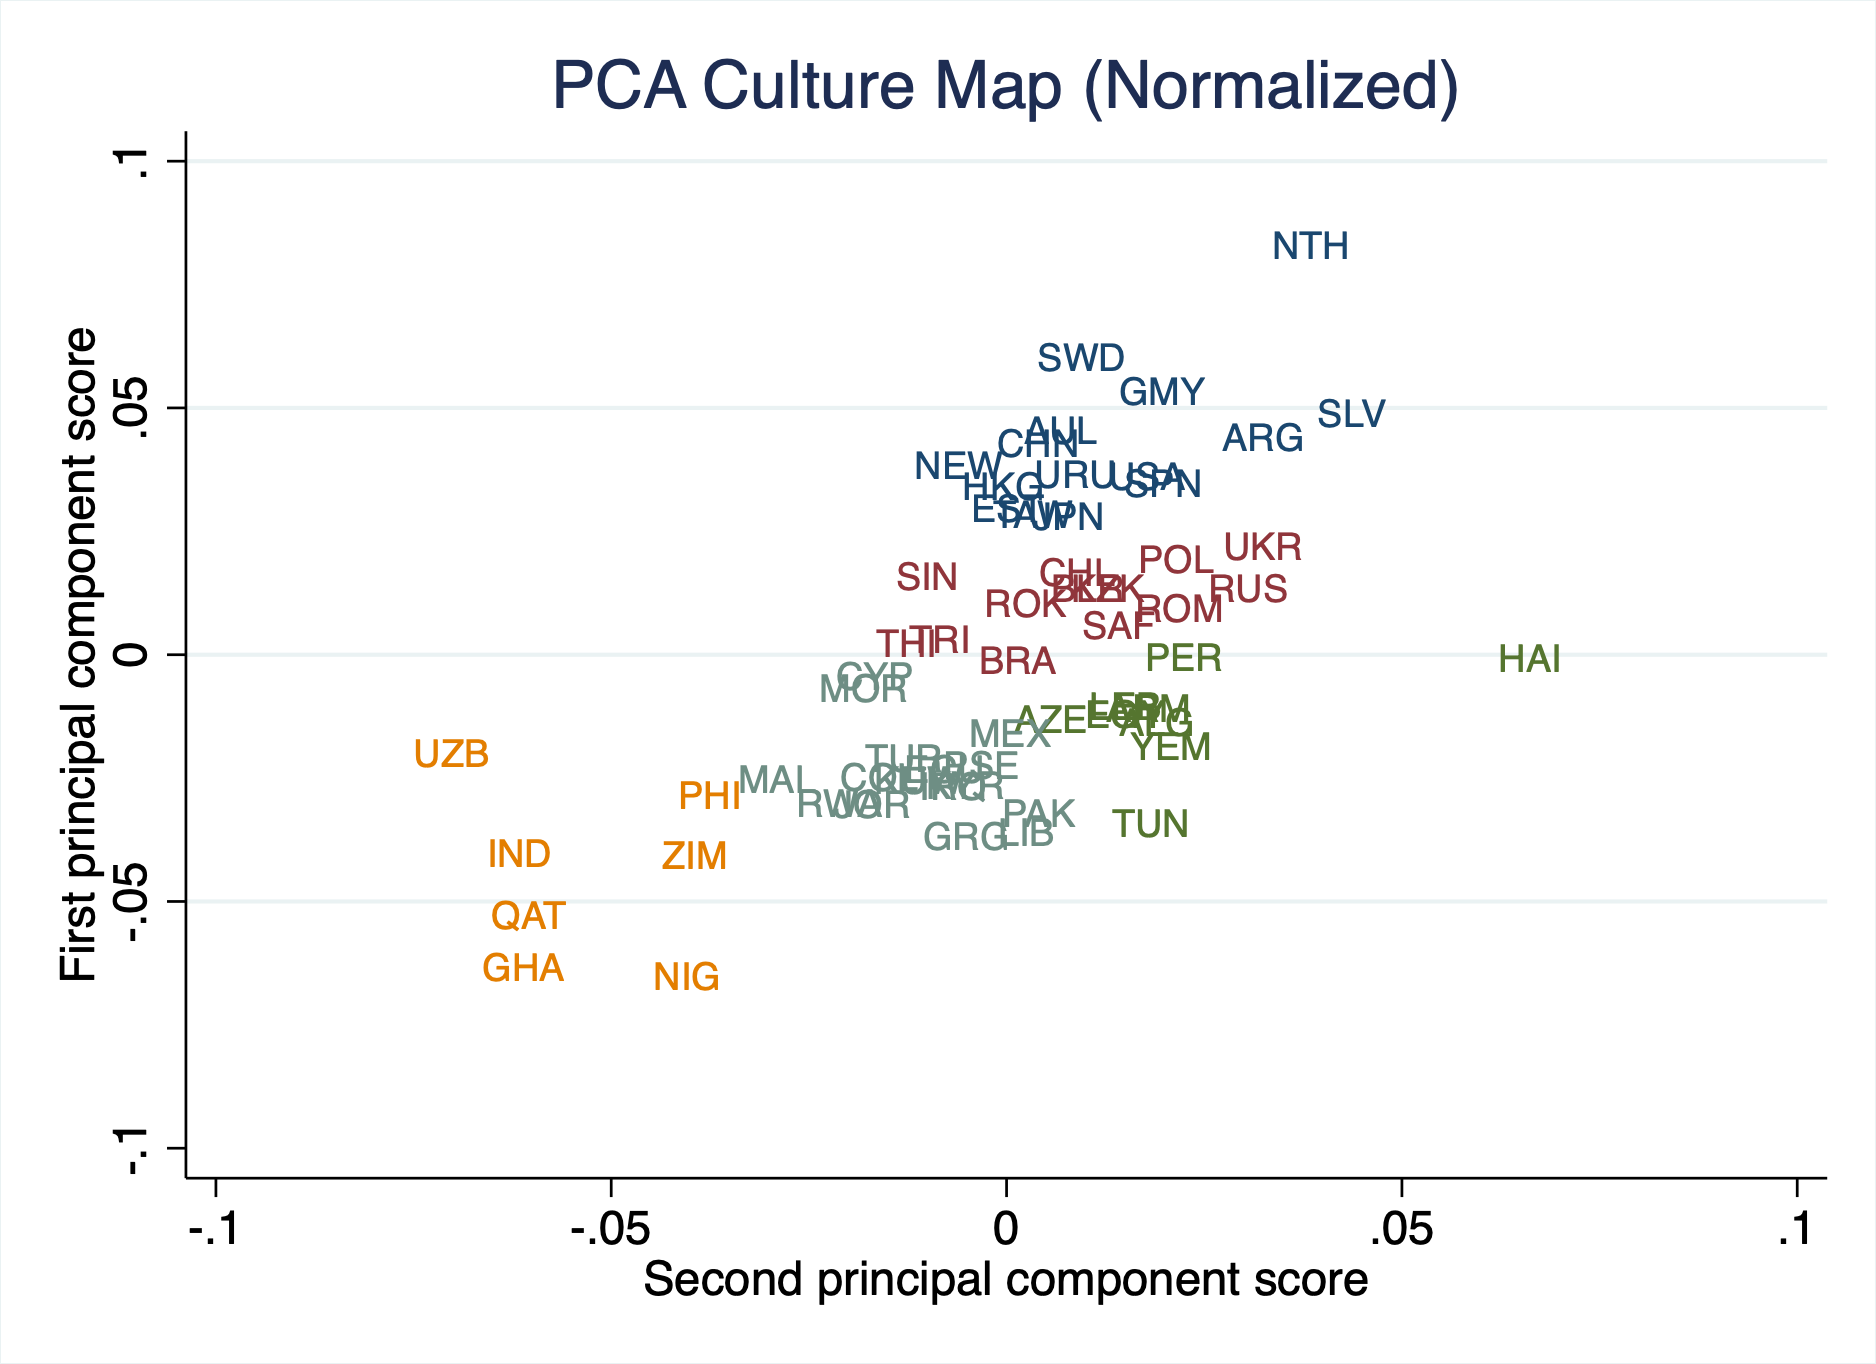
\includegraphics[scale=0.25]{PCA_CultureMap_NOR.png}
\end{center}
The result for the normalized data is similar to that of the non-normalized ones, but a bit more centered towards the mean zero. When seeing Table 2 and 3, there seem to be not much of a difference in terms how the PCA results constituted for the normalized and non-normalized data. 
\end{figure} 

\begin{table}[tbp]
\centering
\caption{PCA factor loading for two components (normalized data)}
\begin{adjustbox}{width=0.7\textwidth}
\small

\begin{tabularx}{\linewidth}{@{}lCC@{}}

\toprule
{Question Code}&{Factor Loading PC1}&{Factor Loading PC2} \tabularnewline
\midrule \addlinespace[\belowrulesep]
V49&.2078106&.0658256 \tabularnewline
V9&.2017511&.0373875 \tabularnewline
V153&.2016577&.0314327 \tabularnewline
V132&.199843&.0211471 \tabularnewline
V205&.1874759&.079644 \tabularnewline
V53&.1823724&.0495819 \tabularnewline
V139&.1805832&.0364045 \tabularnewline
V75&.1788874&.0352874 \tabularnewline
V182&.1774179&.0284611 \tabularnewline
V51&.1764657&.0915946 \tabularnewline
V52&.1737652&.0117149 \tabularnewline
V71&.1696302&.004705 \tabularnewline
V183&.1689363&.0242158 \tabularnewline
V184&.1667707&.0295192 \tabularnewline
V77&.1618756&.0688607 \tabularnewline
V138&.1602611&.1039313 \tabularnewline
V8&.1559734&.0437046 \tabularnewline
V108&.1557414&.1039401 \tabularnewline
V79&.1544669&.0982276 \tabularnewline
V181&.1501807&.0503627 \tabularnewline
V72&.1487002&.0325913 \tabularnewline
V208&.1458341&.090243 \tabularnewline
V190&.1418065&.1053625 \tabularnewline
V76&.1339771&.0371005 \tabularnewline
V188&.1331382&.1314552 \tabularnewline
V209&.1327176&.0259985 \tabularnewline
V207&.1290189&.0856401 \tabularnewline
V6&.1284723&.0459342 \tabularnewline
V195&.1181935&.0424774 \tabularnewline
V133&.1179397&.0268561 \tabularnewline
V136&.1068502&.0415142 \tabularnewline
V191&.1066016&.0818459 \tabularnewline
V189&.105217&.1394171 \tabularnewline
V96&.0965359&.0665168 \tabularnewline
V173&.096088&.1549147 \tabularnewline
V200&.0926921&.1472956 \tabularnewline
V70&.0900791&.0666295 \tabularnewline
V202&.090005&.1505664 \tabularnewline
V171&.0879594&.1521657 \tabularnewline
V210&.0873032&.1249943 \tabularnewline
V126&.0837561&.1363711 \tabularnewline
V4&.0832893&.1597116 \tabularnewline
V156&.0831289&.0105251 \tabularnewline
V174&.0816748&.1234134 \tabularnewline
V97&.0771694&.02775 \tabularnewline
V121&.0719786&.1525045 \tabularnewline
V78&.0700914&.1473734 \tabularnewline
V192&.0679175&.1678085 \tabularnewline
V98&.0647198&.0564803 \tabularnewline
V194&.0646833&.0449819 \tabularnewline
V73&.063028&.0154043 \tabularnewline
V59&.0600082&.0839329 \tabularnewline
V137&.0584312&.0506936 \tabularnewline
V11&.0584005&.0921803 \tabularnewline
V198&.0575535&.0963539 \tabularnewline
V111&.0554647&.1431794 \tabularnewline
V99&.0517413&.1275601 \tabularnewline
V5&.0515413&.0975953 \tabularnewline
V119&.0505839&.1894179 \tabularnewline
V134&.0486164&.0669977 \tabularnewline
V100&.0474854&.1168805 \tabularnewline
V199&.046895&.1595382 \tabularnewline
V113&.0432354&.1974874 \tabularnewline
V7&.0420467&.0563234 \tabularnewline
V120&.0413593&.1927005 \tabularnewline
V123&.0391502&.1555381 \tabularnewline
V196&.0390704&.0715778 \tabularnewline
V122&.0388508&.1572322 \tabularnewline
V110&.0320941&.1464552 \tabularnewline
V193&.0296571&.1585311 \tabularnewline
V55&.0276206&.1280686 \tabularnewline
V54&.0271649&.0957843 \tabularnewline
V155&.0243402&.0559897 \tabularnewline
V115&.0243188&.2031389 \tabularnewline
V170&.0142834&.1656278 \tabularnewline
V197&.0139431&.1389542 \tabularnewline
V101&.0129306&.1452573 \tabularnewline
V124&.0074677&.2014914 \tabularnewline
V10&.0074069&.1022216 \tabularnewline
V114&.0046042&.2051757 \tabularnewline
V131&.0036992&.0142737 \tabularnewline
V117&.0018599&.1779269 \tabularnewline
\bottomrule 

\end{tabularx}


\end{adjustbox}
\end{table}

\end{document}

